%%____________________________________________________________________________||

%%____________________________________________________________________________||
\RCS$Revision: 310950 $
\RCS$HeadURL: svn+ssh://svn.cern.ch/reps/tdr2/notes/AN-15-004/trunk/AN-15-004.tex $
\RCS$Id: AN-15-004.tex 310950 2015-11-17 23:34:16Z sakuma $

%%____________________________________________________________________________||
\newlength\cmsFigWidth
\ifthenelse{\boolean{cms@external}}{\setlength\cmsFigWidth{0.85\columnwidth}}{\setlength\cmsFigWidth{0.4\textwidth}}
\ifthenelse{\boolean{cms@external}}{\providecommand{\cmsLeft}{top\xspace}}{\providecommand{\cmsLeft}{left\xspace}}
\ifthenelse{\boolean{cms@external}}{\providecommand{\cmsRight}{bottom\xspace}}{\providecommand{\cmsRight}{right\xspace}}
%\usepackage{xr}

%%____________________________________________________________________________||
\cmsNoteHeader{AN-15-279}

%%____________________________________________________________________________||
\title{Inclusive WIMP searches using $\alpha_\textrm{T}$ in final states with jets and missing transverse momentum at $\sqrt{s}$ = 13~TeV pp collisions }

%%____________________________________________________________________________||
%\author[bristol]{R.~Aggleton}
\author[imperial]{M.~Baber}
\author[imperial]{R.~Bainbridge}
\author[vub]{F.~Blekman}
\author[imperial]{O.~Buchm\"uller}
\author[bristol]{J.~Brooke}
\author[imperial]{S.~Casasso}
\author[imperial]{M.~Citron}
\author[imperial]{A.~Elwood}
\author[bristol]{H.~Fl\"acher}
\author[rochester]{A.~Garcia-Bellido}
\author[imperial]{C.~Laner}
\author[rochester]{K.H.~Lo}
%\author[bristol]{C.~Lucas}
\author[imperial]{S.A.~Malik}
\author[imperial]{B.~Penning}
\author[bristol]{T.~Sakuma}
\author[vub]{D.~Smith^{1,}}
\author[imperial]{A.~Tapper}

\address[bristol]{University of Bristol, Bristol, UK}
\address[imperial]{Imperial College, London, UK}
\address[vub]{Vrije Universiteit Brussel, Brussel, BE}
\address[rochester]{University of Rochester, NY, US}

%%____________________________________________________________________________||
\date{\today}

%%____________________________________________________________________________||
\abstract{This note summarises an inclusive search for dark matter candidates in
 final states with jets and missing transverse
energy in pp collisions at a centre-of-mass energy of $\sqrt{s}$ =
13~TeV. The search optimizes acceptance for dark matter by performing
a search binned according to the total number of ($b$-)jets in the event and
the scalar sum of the jet energies. 
To account for the different type of possible dark matter signatures we optimize
the jet selection in monojet like events, event with ISR like signatures and 
pair-production of heavy objects.
Two dimensionless variables, \alphat and \bdphi, are used to control QCD multijet and
instrumental effects at the sub-percent level and to enrich events with large missing transverse energy.
We analyse 2.1~$\text{fb}^{-1}$ of data and provide interpretations in minimal simplified dark matter models.
}

%%____________________________________________________________________________||
\hypersetup{ 
  pdfauthor={Robin Aggleton, Mark Baber, Robert Bainbridge, Freya
Blekman, Oliver Buchmueller, Jim Brooke, Stefano Casasso, Matthew
Citron, Adam Elwood, Henning Flaecher, Aran Garcia-Bellido, Christian
Laner, Kin Ho Lo, Chris Lucas, Sarah Alam Malik, Bjoern Penning, Tai
Sakuma, Dominic Smith, Alex Tapper.},
  pdftitle={Search for new physics in final states with jets and missing
  transverse momentum in 13 TeV pp collisions with the AlphaT variable:
  the Early Analysis exercise},
  pdfsubject={CMS, jets, missing transverse momentum, supersymmetry,
  dark matter, AlphaT},
  pdfkeywords={CMS, jets, missing transverse momentum, supersymmetry,
  dark matter, AlphaT},
}

%%____________________________________________________________________________||
\maketitle

%%____________________________________________________________________________||
\tableofcontents

%%____________________________________________________________________________||
\newcommand{\eslash}{{\hbox{$E$\kern-0.6em\lower-.05ex\hbox{/}\kern0.10em}}}
\newcommand{\met}{\mbox{$\eslash_\text{T}$}\xspace}
\newcommand{\cls}{\mbox{CL$_s$}\xspace}
\newcommand{\wtaunu}{\ensuremath{\PW \rightarrow \Pgt\cPgn}}
\newcommand{\Et}{\ensuremath{{E_{\text T}}}\xspace}
\newcommand{\Hslash}{{\hbox{$H$\kern-0.8em\lower-.05ex\hbox{/}\kern0.10em}}}

\newcommand{\scalht}{\mbox{$H_\text{T}$}\xspace}
\newcommand{\mht}{\mbox{$\Hslash_\text{T}$}\xspace}
\newcommand{\HTmiss}{\mbox{$H_\text{T}^\text{miss}$}\xspace}
\newcommand{\dht}{\ensuremath{\Delta\scalht}\xspace}
\newcommand{\alphat}{\ensuremath{\alpha_{\text T}}\xspace}
\newcommand{\njet}{\ensuremath{N_{\text{jet}}}\xspace}
\newcommand{\njetlow}{\ensuremath{2 \leq \njet \leq 3}\xspace}
\newcommand{\njethigh}{\ensuremath{\njet \geq 4}\xspace}
\newcommand{\nb}{\ensuremath{N_{\text{b}}}\xspace}
\newcommand{\mj}{\ensuremath{\mu\! +\! \text{jets}}\xspace}
\newcommand{\mmj}{\ensuremath{\mu\mu\! +\! \text{jets}}\xspace}
\newcommand{\gj}{\ensuremath{\gamma\! +\! \text{jets}}\xspace}
\newcommand{\wjets}{\ensuremath{\PW\! +\! \text{jets}}\xspace}
\newcommand{\zjets}{\ensuremath{\cPZ\! +\! \text{jets}}\xspace}
\newcommand{\znunujets}{\ensuremath{\cPZ\! \rightarrow\! \cPgn\cPagn\! +\! \text{jets}}\xspace}
\newcommand{\znunu}{\ensuremath{\cPZ\! \rightarrow\! \cPgn\cPagn}\xspace}
\newcommand{\zmumu}{\ensuremath{\cPZ\! \rightarrow\! \mu\mu}\xspace}
\newcommand{\zmumujets}{\ensuremath{\cPZ\! \rightarrow\! \mu\mu\! +\! \text{jets}}\xspace}
\newcommand\T{\rule{0pt}{2.6ex}}
\newcommand\B{\rule[-1.2ex]{0pt}{0pt}}
\def\mhtmet{\mbox{$\HTmiss / \ETmiss$}\xspace}
\newcommand{\Pt}{\ensuremath{{p_{\text T}}}\xspace}
\newcommand{\dphi}{\ensuremath{\Delta\phi^{*}_\text{min}}\xspace}
\newcommand{\dm}{\ensuremath{\Delta m}\xspace}
\newcommand{\alphatmin}{\ensuremath{\alphat^\text{min}}\xspace}

\newcommand\rs{\raisebox{1.0ex}[-1.0ex]}

% PROCESSES

\newcommand{\ra}{\ensuremath{\rightarrow}}
\newcommand{\jets}{\ensuremath{\text{jets}}}

\newcommand{\lj}{\ensuremath{\ell\! +\! \jets}\xspace}
\newcommand{\mj}{\ensuremath{\mu\! +\! \jets}\xspace}
\newcommand{\ej}{\ensuremath{e\! +\! \jets}\xspace}

\newcommand{\llj}{\ensuremath{\ell\ell\! +\! \jets}\xspace}
\newcommand{\mmj}{\ensuremath{\mu\mu\! +\! \jets}\xspace}
\newcommand{\eej}{\ensuremath{ee\! +\! \jets}\xspace}
\newcommand{\mmjpm}{\ensuremath{\mu^\pm\mu^\mp\! +\! \jets}\xspace}

\newcommand{\gj}{\ensuremath{\gamma\! +\! \jets}\xspace}

\newcommand{\wj}{\ensuremath{\PW\! +\! \jets}\xspace}
\newcommand{\wlj}{\ensuremath{\PW\! (\ra\! \ell\nu)\! +\! \textrm{jets}}\xspace}
\newcommand{\wmj}{\ensuremath{\PW\! (\ra\! \mu\nu)\! +\! \textrm{jets}}\xspace}
\newcommand{\wej}{\ensuremath{\PW\! (\ra\! e\nu)\! +\! \textrm{jets}}\xspace}

\newcommand{\wlnu}{\ensuremath{\PW\! \ra\! \ell\nu}\xspace}
\newcommand{\wmunu}{\ensuremath{\PW\! \ra\! \mu\nu}\xspace}
\newcommand{\wenu}{\ensuremath{\PW\! \ra\! e\nu}\xspace}
\newcommand{\wtaunu}{\ensuremath{\PW \rightarrow \Pgt\cPgn}\xspace}

\newcommand{\zj}{\ensuremath{\cPZ\! +\! \jets}\xspace}
\newcommand{\zllj}{\ensuremath{\cPZ\! (\ra\! \ell\ell)\! + \! \jets}\xspace}
\newcommand{\zmumuj}{\ensuremath{\cPZ\! (\ra\! \mu\mu)\! +\! \jets}\xspace}
\newcommand{\zeej}{\ensuremath{\cPZ\! (\ra\! ee)\! +\! \jets}\xspace}
\newcommand{\znunuj}{\ensuremath{\cPZ\! (\ra\! \cPgn\cPagn)\! +\! \jets}\xspace}

\newcommand{\zll}{\ensuremath{\cPZ\! \ra\! \ell\ell}\xspace}
\newcommand{\zmumu}{\ensuremath{\cPZ\! \ra\! \mu\mu}\xspace}
\newcommand{\zee}{\ensuremath{\cPZ\! \ra\! ee}\xspace}
\newcommand{\znunu}{\ensuremath{\cPZ\! \ra\! \cPgn\cPagn}\xspace}

\newcommand{\ttj}{\ensuremath{\ttbar\! +\! \jets}\xspace}
\newcommand{\ttw}{\ensuremath{\ttbar\PW}\xspace}
\newcommand{\ttz}{\ensuremath{\ttbar\cPZ}\xspace}

% SIGNAL 

\newcommand{\Ttwocc}{\ensuremath{\text{pp}\,\ra\,\sTop\sTop^{*}\,\ra\,\text{c}\chiz\,\bar{\text{c}}\chiz}}
\newcommand{\Ttwodegen}{\ensuremath{\text{pp}\,\ra\,\sTop\sTop^{*}\,\ra\,\text{b}ff'\chiz \,\text{b}ff'\chiz}}
\newcommand{\Ttwobw}{\ensuremath{\text{pp}\,\ra\,\sTop\sTop^{*}\,\ra\,\text{b}W\chiz \,\bar{\text{b}}W\chiz}}
\newcommand{\Ttwott}{\ensuremath{\text{pp}\,\ra\,\sTop\sTop^{*}\,\ra\,\text{t}\chiz\,\bar{\text{t}}\chiz}}
\newcommand{\Ttwobb}{\ensuremath{\text{pp}\,\ra\,\sBot\sBot^{*}\,\ra\,\text{b}\chiz\,\bar{\text{b}}\chiz}}
\newcommand{\Ttwoqq}{\ensuremath{\text{pp}\,\ra\,\sQua\sQua^{*}\,\ra\,\text{q}\chiz\,\bar{\text{q}}\chiz}}
\newcommand{\Tonebbbb}{\ensuremath{\text{pp}\,\ra\,\sGlunew\sGlunew^{*}\,\ra\,\bar{\text{b}}\text{b}\chiz\,\bar{\text{b}}\text{b}\chiz}}
\newcommand{\Toneqqqq}{\ensuremath{\text{pp}\,\ra\,\sGlunew\sGlunew^{*}\,\ra\,\bar{\text{q}}\text{q}\chiz\,\bar{\text{q}}\text{q}\chiz}}
\newcommand{\Tonetttt}{\ensuremath{\text{pp}\,\ra\,\sGlunew\sGlunew^{*}\,\ra\,\bar{\text{t}}\text{t}\chiz\,\bar{\text{t}}\text{t}\chiz}}

%\newcommand{\dphi}{\ensuremath{\Delta \phi}}
\newcommand{\dphi}{\ensuremath{\Delta\phi^{*}_{\rm min}}\xspace}
\newcommand{\dphijj}{\ensuremath{\Delta \phi_{ j1,j2}}}
\newcommand{\Pt}{\ensuremath{{p_{\text T}}}\xspace}
\newcommand{\pts}{\ensuremath{p_{\text T}{\text s}}\xspace}
\newcommand{\Et}{\ensuremath{{E_{\text T}}}\xspace}
\newcommand{\ptjf}{\ensuremath{p_{\rm T}^{ {\rm j}_1} }}
\newcommand{\ptjs}{\ensuremath{p_{\rm T}^{ {\rm j}_2} }}
\newcommand{\ptjt}{\ensuremath{p_{\rm T}^{ {\rm j}_3} }}
\newcommand{\etajf}{\ensuremath{\eta^{ {\rm j}_1} }}
\newcommand{\etajs}{\ensuremath{\eta^{ {\rm j}_2} }}
\newcommand{\etajt}{\ensuremath{\eta^{ {\rm j}_3} }}
\newcommand{\al}{\ensuremath{\alpha}}
\newcommand{\alt}{\ensuremath{\alpha_{\text{T}}}\xspace}
\newcommand{\etaabs}{\ensuremath{|\eta|}}
%\newcommand{\gev}{\ensuremath{\mathrm{\,Ge\kern -0.1em V}}}
\newcommand{\pb}{\ensuremath{pb^{-1}}}
\newcommand{\mjj}{\ensuremath{M_{\text{inv}}^{j1,j2}}}
\newcommand{\chiznew}{\ensuremath{\chi^{0}}\xspace}
\newcommand{\chipnew}{\ensuremath{\chi^{+}}\xspace}
\newcommand{\sQuanew}{\ensuremath{\tilde{\rm q}}\xspace}
\newcommand{\sGlunew}{\ensuremath{\tilde{\rm g}}\xspace}
\newcommand{\ttNew}{\ensuremath{\rm{t}\bar{\rm{t}}}\xspace}
\newcommand{\tev}{\TeV}
%<TW date="30/10/2010">
%\newcommand{\Et}{E_{T}}
\newcommand{\combIso}{Iso_{\textrm{comb.}}}
\renewcommand{\arraystretch}{1.2}
\newcommand{\bigNum}[2]{#1 \, \times \, 10 \, ^{#2}}
%</TW>

\newcommand{\raT}{\ensuremath{R_{\alt}}}
\newcommand{\RaT}{\ensuremath{R_{\alt}}\xspace}

\newcommand\T{\rule{0pt}{2.6ex}}
\newcommand\B{\rule[-1.2ex]{0pt}{0pt}}

\def\eslash{{\hbox{$E$\kern-0.6em\lower-.05ex\hbox{/}\kern0.10em}}}
\def\vecmet{\mbox{$\vec{\eslash}_T$}} %missing ET vector
\def\vecet{\mbox{$\vec{E}_\text{T}$}} % ET vector
\def\MET{\mbox{$\eslash_\text{T}$}\xspace}
%\def\met{\mbox{$\eslash_\text{T}$}\xspace}
\def\met{\mbox{$E_\text{T}^{\rm miss}$}\xspace}
\def\pfmet{\mbox{$\eslash_\text{T}^{\rm PF}$}\xspace}
\def\mex{\mbox{$\eslash_\text{x}$}} %missing Ex
\def\mey{\mbox{$\eslash_\text{y}$}} %missing Ey
\def\mepar{\mbox{$\eslash_\parallel$}}
\def\meperp{\mbox{$\eslash_\perp$}}
\def\Zmm{Z \rightarrow \mu\mu}
\def\metvec{\mbox{$\vec{\met}$}\xspace}
\def\metvecrec{\mbox{$\vec{\met}^{\rm rec}$}\xspace}
\def\metvecgen{\mbox{$\vec{\met}^{\rm gen}$}\xspace}
\def\metgen{\mbox{$\met^{\rm gen}$}\xspace}
\def\metparl{\mbox{$\mepar^{\rm rec}$}\xspace}
\def\metperp{\mbox{$\meperp^{\rm rec}$}\xspace}
\def\deltamet{\mbox{$\Delta\met$}\xspace}
\def\pthat{\mbox{$\hat{p}_T$}\xspace}
\def\hslash{{\hbox{$H$\kern-0.8em\lower-.05ex\hbox{/}\kern0.10em}}}
%\def\MHT{\mbox{$\hslash_\text{T}$}\xspace}
\def\mht{\mbox{$\hslash_\text{T}$}\xspace}
%\def\mht{\mbox{$H_{\rm T}^{\rm miss}$}\xspace}
\newcommand{\HTmiss}{\ensuremath{H_{\text{T}}^{\text{miss}}}\xspace}
\newcommand{\HTmissvec}{\ensuremath{\vec{H_{\text{T}}}^{\text{miss}}}\xspace}
\def\mhtvec{\mbox{$\vec{H}_{\rm T}^{\rm miss}$}\xspace}
%\def\mhtmet{\mbox{$\hslash_\text{T} / \eslash_\text{T}$}\xspace}
%\def\mhtmet{\mbox{$\mht / \met$}\xspace}
\newcommand{\mhtmet}{\ensuremath{H_{\mathrm{T}}^{\text{miss}} / E_{\mathrm{T}}^{\text{miss}}}\xspace}
\def\mhtmetmiss{\mbox{$\H_\text{T}^{\rm miss} / \E_\text{T}^{\rm miss}$}\xspace}
%\def\rmhtmet{\mbox{$R_{\hslash_\text{T} / \eslash_\text{T}}$}\xspace}
\def\rmhtmet{\mbox{$R_{\mht / \met}$}\xspace}
\def\sumet{\mbox{$\sum \rm{E}_\text{T}$}\xspace}
\def\etmiss{\mbox{$\eslash_\text{T}$}\xspace}
\def\htmiss{\mbox{$\hslash_\text{T}$}\xspace}
\def\mtt{\mbox{$\rm{M}_\text{T2}$}\xspace}
\def\rmec{\mbox{$R_{\mht/\met}$}\xspace}
\def\bdphi{\mbox{$\Delta\phi^{*}_{\rm min}$}\xspace}
\def\bdphimod{\mbox{$\Delta\phi^{*_{\, 25}}_{\rm min}$}\xspace}
\def\bigeslash{{\hbox{$E$\kern-0.38em\lower-.05ex\hbox{/}\kern0.10em}}}
\def\bigmet{\mbox{$\bigeslash_T$}}
\def\bighslash{{\hbox{$H$\kern-0.6em\lower-.05ex\hbox{/}\kern0.10em}}}
\def\bigmht{\mbox{$\bighslash_T$}}
\def\incl{\includegraphics[width=0.49\linewidth]}
\def\inclrot{\includegraphics[angle=90,width=0.47\linewidth]}
\def\INCL{\includegraphics[angle=90,width=0.45\linewidth]}
\def\Incl{\includegraphics[angle=90,width=0.60\linewidth]}
\def\cls{\mbox{CL$_s$}\xspace}

\newcommand{\zero}{\ensuremath{\phantom{0}}}

\newcommand{\scalht}{\ensuremath{H_{\mathrm{T}}}\xspace}
\newcommand{\dm}{\ensuremath{\Delta m}\xspace}


%%____________________________________________________________________________||
%%____________________________________________________________________________||
\section{Introduction}
\label{sec:intro}

In this note we summarise the search for WIMPs using the optimised RA1 analysis. The full analsyis documentation consists of two parts. Analysis approach, background estimation and systematic uncertainties are explained in great detail in the RA1 note~\cite{alphaTnote}. This document focuses on the WIMP interpretation.

While to date it is unkown if or in which way a DM candidate is produced at collider we can parameterise the various phyiscal possibilities. In many models the production of a hadronic particlel can be postules, either from initial- or final-state radiation or from associated production with a boson or quarks.
A large missing transverse momentum (\MET) is introduced to the event by the DM candidate escaping the detector undetected. Therefore one has to study $\etmiss$ plus jet final states emphasizing acceptance and low kinematics to account for a large range of possible kinmeatics. These range from low jets multiplicities and low energies to large masses, jet multiplicities and possibbly $b$-quark jets.

We consider all available topologies - mono-jet, multi-jet and heavy quarks - in one analysis. 

Using two special kinematic variables,  $\alpha_{\textrm T}$ and $\bdphi$ we maximise sensitivity while maintaining high purity for events with real missing transverse energy.
The \alphat variable allows to to efficiently select candidate signal events with genuine \MET while
providing robust rejection against background events from QCD multijet production. Further reduction of QCD multijet and instrumental background is achieved using the $\dphi$ variable.

This is an evolution of past searches for supersymmetry (SUSY) in proton-proton collisions data collected during LHC Run~1. With data at a centre-of-mass energy of 7 TeV collected in 2010 and 2011, the \alphat analysis has excluded a large parameter space of the constrained minimal supersymmetric extension of the standard model (CMSSM) \cite{Khachatryan:2011tk, Chatrchyan:2011zy, Chatrchyan:2012wa} and a parameter space of simplified models \cite{Chatrchyan:2012wa}. With data at a centre-of-mass energy of 8 TeV collected and promptly reconstructed in 2012, the \alphat analysis
further excluded a parameter space of simplified models \cite{Chatrchyan:2013lya}.  The search strategy in this note is an extension of that in Ref. \cite{CMS_AN_2013-366}.

With the start of Run 2 in June 2015 the LHC delivers proton-proton collisions at a higher centre-of-mass energy of 13 TeV. The higher energy collision considerably increases the production cross sections of possible dark matter processes. Members of this analysis team have been pivotal in establishing a set of 'Minimal Simplified Dark Matter' models and usage recommendations in the 'ATLAS-CMS-DM-Forum' for Run 2 of the LHC. This experience guided choice and optimisation in this particularly suited search for DM.

\section{Analysis Strategy and the \alphat variable}

The goal of this RA1 DM search is to be sensitive to a large range of potential DM models. The guiding principles are low thresholds, maximal coverage, robustness in early data and negligible QCD multijet backgrounds.

Approximate kinematic thresholds of this analysis are:

\begin{itemize}
   \item  $H_\textrm{T}>200$~GeV
   \item  $H^{miss}_\textrm{T}>130$~GeV
   \item  $p_\textrm{T}(j)>40$~GeV
\end{itemize}

The analysis uses the \alphat~\cite{Randall:2008rw, CMS:2008vya, CMS-PAS-SUS-09-001} variable to
 efficiently reject multijet events without significant \met or with transverse energy mismeasurements, 
while retaining a large sensitivity to new physics with final-state signatures containing significant \met.

For dijet events, the \alphat variable is defined as:

\begin{equation}
\label{eq:alphat}
\alphat\, =\, \frac{\Et^{{\rm j}_2}}{M_\text{T}} \, ,
\end{equation}

where $\Et^{\rm j_2}$ is the transverse energy of the less energetic
jet and $M_\text{T}$ is the transverse mass of the dijet system,
defined as

\begin{equation}
  \label{eq:mt}
  M_\text{T}\, = \,\sqrt{ \left( \sum_{i=1}^2 \Et^{{\rm j}_i}
    \right)^2 - \left( \sum_{i=1}^2 p_x^{{\rm j}_i} \right)^2 - \left(
      \sum_{i=1}^2 p_y^{{\rm j}_i} \right)^2} \, .
\end{equation}

where $\Et^{{\rm j}_i}$, $p_x^{{\rm j}_i}$, and $p_y^{{\rm j}_i}$ are,
respectively, the transverse energy and $x$ or $y$ components of the
transverse momentum of jet ${\rm j}_i$.

For a perfectly dijet event with $\Et^{\rm j_1} = \Et^{\rm j_2}$ and back-to-back jets in $\phi$, and in the limit in which the
momentum of each jet is large compared with its mass, the value of \alphat becomes 0.5. If there is an imbalance in the measured
transverse energies of back-to-back jets, \alphat is reduced to a value smaller than 0.5, which gives rise to the variables intrinsic
robustness against jet energy mismeasurements. Values significantly greater than 0.5 are observed when the two jets are not 
back-to-back and are recoiling against significant, genuine \met.

The definition of the \alphat variable can be generalised for events with two or more jets as follows. The mass scale of the physics
processes being probed is characterised by the scalar sum of the transverse energy $\Et$ of jets considered in the analysis, defined as
$\scalht = \sum_{i=1}^{\njet} \Et^{{\rm j}_i}$, where \njet is the number of jets with \Et above a predefined threshold. The estimator
for \met is given by the magnitude of the transverse momenta $\vec{\pt}$ vectorial sum over these jets, defined as $\mht =
|\sum_{i=1}^{N_{\rm jet}} \vec{\pt}^{{\rm j}_i}|$. 

For events with three or more jets, a pseudo-dijet system is formed by combining the jets in the event into two pseudo-jets. The total \Et
for each of the two pseudo-jets is calculated as the scalar sum of the measured \Et of the contributing jets. The combination chosen is the
one that minimises the absolute \Et difference between the two pseudo-jets, \dht. This simple clustering criterion provides the best
separation between multijet events and events with genuine \met. Eq.~\ref{eq:alphat} can therefore be generalised as:

\begin{equation}
  \label{eq:alphat2}
  \alphat\, = \,\frac{1}{2} \times \frac{\scalht -
    \dht}{\sqrt{\scalht^2 - \mht^2}} \, = \,\frac{1}{2} \times 
  \frac{1 - (\dht/\scalht)}{\sqrt{1 - (\mht/\scalht)^2}} \, . 
\end{equation}

In the presence of jet energy mismeasurements, the direction and magnitude of the apparent missing transverse energy, \mht, and energy
imbalance of the pseudo-dijet system, \dht, are highly correlated. This correlation is much weaker for R-parity-conserving SUSY with each
of the two decay chains producing the LSP. It is useful to consider the limiting case $\dht \rightarrow 0$ to
understand the relationship between \alphat and the ratio \mht/\scalht:

\begin{equation}
  \label{eq:alphat3}
  \frac{\mht}{\scalht} \, = \, \sqrt{ 1 - \frac{1}{4 \cdot \alphat^2} }
\end{equation}

For reference, under the assumption of $\dht = 0$, the values of
$\alphat = 0.55$, 0.60, and 0.65 map onto values of the ratio
$\mht/\scalht = 0.42$, 0.55, and 0.64.


%%____________________________________________________________________________||
\section{Data sets}
\label{sec:datasets}

\subsection{Data}


In this note, we use 36.4~\ifb of proton-proton collision data at
$\sqrt{s} =$ 13~TeV collected in 2016. The JSON file listed in
Table~\ref{tab:cert_json} specifies the periods of the time in which
these certified data are collected. Table~\ref{tab:datasets_data} lists
the names of the data sets.

We perform a blind analysis. The data in the signal region is
currently blinded with the exception of 5.2~\ifb of the certified data
in Run2016G, as recommended by the SUS PAG. We have intentionally not
unblinded the ICHEP data set. The control regions are populated with
the full 2016 data set.

\begin{table}[!h]
  \topcaption{The JSON file used to specify the certified data set of
    36.4~\ifb} 
  \footnotesize
  %latex.default(d, title = NULL, booktabs = FALSE, width = 3, rowname = NULL,     helvetica = FALSE, caption.loc = "bottom", ...)%
\begin{center}
\begin{tabular}{c}
\hline\hline
\verb!Cert_246908-258750_13TeV_PromptReco_Collisions15_25ns_JSON.txt!\tabularnewline
\hline
\end{tabular}\end{center}
 
  \label{tab:cert_json}
\end{table}

\begin{table}[!h]
  \topcaption{Data sets}
  \footnotesize %latex.default(d, title = NULL, booktabs = FALSE, width = 3, rowname = NULL,     helvetica = FALSE, caption.loc = "bottom", ...)%
\begin{center}
\begin{tabular}{lr}
\hline\hline
\multicolumn{1}{c}{Data set}&\multicolumn{1}{c}{$\int\mathcal{L}\textrm{d}t [\textrm{pb}^{-1}]$}\tabularnewline
\hline
\verb!/HTMHT/Run2015D-05Oct2015-v1/MINIAOD! &$ 551.60$\tabularnewline
\verb!/HTMHT/Run2015D-PromptReco-v4/MINIAOD! &$1599.66$\tabularnewline
\verb!/JetHT/Run2015D-05Oct2015-v1/MINIAOD! &$ 552.67$\tabularnewline
\verb!/JetHT/Run2015D-PromptReco-v4/MINIAOD! &$1599.66$\tabularnewline
\verb!/MET/Run2015D-05Oct2015-v1/MINIAOD! &$ 552.67$\tabularnewline
\verb!/MET/Run2015D-PromptReco-v4/MINIAOD! &$1599.66$\tabularnewline
\verb!/SingleElectron/Run2015D-05Oct2015-v1/MINIAOD! &$ 552.63$\tabularnewline
\verb!/SingleElectron/Run2015D-PromptReco-v4/MINIAOD! &$1599.11$\tabularnewline
\verb!/SingleMuon/Run2015D-05Oct2015-v1/MINIAOD! &$ 552.67$\tabularnewline
\verb!/SingleMuon/Run2015D-PromptReco-v4/MINIAOD! &$1599.53$\tabularnewline
\verb!/SinglePhoton/Run2015D-05Oct2015-v1/MINIAOD! &$ 552.67$\tabularnewline
\verb!/SinglePhoton/Run2015D-PromptReco-v4/MINIAOD! &$1598.83$\tabularnewline
\hline
\end{tabular}\end{center}

  \label{tab:datasets_data}
\end{table}

%% \begin{table}[!h]
%% \topcaption{The JSON file specifying the 0.8~\ifb of the certified
%% data that we never blind} \footnotesize
%% \input{tables/datasets/cert_unblind_json.tex}
%% \label{tab:cert_unblind_json}
%% \end{table}

\subsection{Simulation}

Table~\ref{tab:datasets_bkg} lists the data sets of simulated events
of the standard model background processes used in this note. In these
data sets, in addition to the main interaction, each event contains on
average 20 minimum bias interactions which simulate multiple
interactions per bunch-crossing (in-time pileup). The expected
detector signal from previous or following bunch crossings
(out-of-time pileup) with 25ns bunch spacing is also overlaid.

\begin{table}[!h]
  \centering
  \topcaption{Simulated background samples}
  \tiny
  \scalebox{.7}[1.0]{%latex.default(d, title = NULL, booktabs = FALSE, width = 3, rowname = NULL,     helvetica = FALSE, caption.loc = "bottom", ...)%
\begin{center}
\begin{tabular}{ll}
\hline\hline
\multicolumn{1}{c}{Data set}&\multicolumn{1}{c}{Cross section [pb]}\tabularnewline
\hline
\verb!/TT_TuneCUETP8M1_13TeV-powheg-pythia8/RunIISpring16MiniAODv2-PUSpring16_80X_mcRun2_asymptotic_2016_miniAODv2_v0_ext4-v1/MINIAODSIM! &$8.318\times 10^{+02}$\tabularnewline
\verb!/TTJets_HT-600to800_TuneCUETP8M1_13TeV-madgraphMLM-pythia8/RunIISpring16MiniAODv2-PUSpring16_80X_mcRun2_asymptotic_2016_miniAODv2_v0_ext1-v1/MINIAODSIM! &$2.667\times 10^{+00}$\tabularnewline
\verb!/TTJets_HT-800to1200_TuneCUETP8M1_13TeV-madgraphMLM-pythia8/RunIISpring16MiniAODv2-PUSpring16_80X_mcRun2_asymptotic_2016_miniAODv2_v0_ext1-v1/MINIAODSIM! &$1.098\times 10^{+00}$\tabularnewline
\verb!/TTJets_HT-1200to2500_TuneCUETP8M1_13TeV-madgraphMLM-pythia8/RunIISpring16MiniAODv2-PUSpring16_80X_mcRun2_asymptotic_2016_miniAODv2_v0_ext1-v1/MINIAODSIM! &$1.987\times 10^{-01}$\tabularnewline
\verb!/TTJets_HT-2500toInf_TuneCUETP8M1_13TeV-madgraphMLM-pythia8/RunIISpring16MiniAODv2-PUSpring16_80X_mcRun2_asymptotic_2016_miniAODv2_v0-v1/MINIAODSIM! &$2.368\times 10^{-03}$\tabularnewline
\verb!/TTJets_SingleLeptFromT_TuneCUETP8M1_13TeV-madgraphMLM-pythia8/RunIISpring16MiniAODv2-PUSpring16_80X_mcRun2_asymptotic_2016_miniAODv2_v0-v1/MINIAODSIM! &$1.827\times 10^{+02}$\tabularnewline
\verb!/TTJets_SingleLeptFromTbar_TuneCUETP8M1_13TeV-madgraphMLM-pythia8/RunIISpring16MiniAODv2-PUSpring16_80X_mcRun2_asymptotic_2016_miniAODv2_v0-v1/MINIAODSIM! &$1.827\times 10^{+02}$\tabularnewline
\verb!/TTJets_SingleLeptFromTbar_TuneCUETP8M1_13TeV-madgraphMLM-pythia8/RunIISpring16MiniAODv2-PUSpring16_80X_mcRun2_asymptotic_2016_miniAODv2_v0_ext1-v1/MINIAODSIM! &$1.827\times 10^{+02}$\tabularnewline
\verb!/TTJets_DiLept_TuneCUETP8M1_13TeV-madgraphMLM-pythia8/RunIISpring16MiniAODv2-PUSpring16_80X_mcRun2_asymptotic_2016_miniAODv2_v0_ext1-v1/MINIAODSIM! &$8.829\times 10^{+01}$\tabularnewline
\verb!/WJetsToLNu_TuneCUETP8M1_13TeV-madgraphMLM-pythia8/RunIISpring16MiniAODv1-PUSpring16_80X_mcRun2_asymptotic_2016_v3-v2/MINIAODSIM! &$6.153\times 10^{+04}$\tabularnewline
\verb!/WJetsToLNu_HT-100To200_TuneCUETP8M1_13TeV-madgraphMLM-pythia8/RunIISpring16MiniAODv2-PUSpring16_80X_mcRun2_asymptotic_2016_miniAODv2_v0_ext1-v1/MINIAODSIM! &$1.627\times 10^{+03}$\tabularnewline
\verb!/WJetsToLNu_HT-200To400_TuneCUETP8M1_13TeV-madgraphMLM-pythia8/RunIISpring16MiniAODv2-PUSpring16_80X_mcRun2_asymptotic_2016_miniAODv2_v0_ext1-v1/MINIAODSIM! &$4.352\times 10^{+02}$\tabularnewline
\verb!/WJetsToLNu_HT-400To600_TuneCUETP8M1_13TeV-madgraphMLM-pythia8/RunIISpring16MiniAODv2-PUSpring16_80X_mcRun2_asymptotic_2016_miniAODv2_v0-v1/MINIAODSIM! &$5.918\times 10^{+01}$\tabularnewline
\verb!/WJetsToLNu_HT-600To800_TuneCUETP8M1_13TeV-madgraphMLM-pythia8/RunIISpring16MiniAODv2-PUSpring16_80X_mcRun2_asymptotic_2016_miniAODv2_v0-v1/MINIAODSIM! &$1.458\times 10^{+01}$\tabularnewline
\verb!/WJetsToLNu_HT-800To1200_TuneCUETP8M1_13TeV-madgraphMLM-pythia8/RunIISpring16MiniAODv2-PUSpring16_80X_mcRun2_asymptotic_2016_miniAODv2_v0_ext1-v1/MINIAODSIM! &$6.656\times 10^{+00}$\tabularnewline
\verb!/WJetsToLNu_HT-1200To2500_TuneCUETP8M1_13TeV-madgraphMLM-pythia8/RunIISpring16MiniAODv2-PUSpring16_80X_mcRun2_asymptotic_2016_miniAODv2_v0-v1/MINIAODSIM! &$1.608\times 10^{+00}$\tabularnewline
\verb!/WJetsToLNu_HT-2500ToInf_TuneCUETP8M1_13TeV-madgraphMLM-pythia8/RunIISpring16MiniAODv2-PUSpring16_80X_mcRun2_asymptotic_2016_miniAODv2_v0-v1/MINIAODSIM! &$3.891\times 10^{-02}$\tabularnewline
\verb!/ZJetsToNuNu_HT-100To200_13TeV-madgraph/RunIISpring15DR74-Asympt25ns_MCRUN2_74_V9-v1/MINIAODSIM! &$3.450\times 10^{+02}$\tabularnewline
\verb!/ZJetsToNuNu_HT-200To400_13TeV-madgraph/RunIISpring15DR74-Asympt25ns_MCRUN2_74_V9-v1/MINIAODSIM! &$9.638\times 10^{+01}$\tabularnewline
\verb!/ZJetsToNuNu_HT-400To600_13TeV-madgraph/RunIISpring15DR74-Asympt25ns_MCRUN2_74_V9-v1/MINIAODSIM! &$1.346\times 10^{+01}$\tabularnewline
\verb!/ZJetsToNuNu_HT-600ToInf_13TeV-madgraph/RunIISpring15DR74-Asympt25ns_MCRUN2_74_V9-v1/MINIAODSIM! &$5.170\times 10^{+00}$\tabularnewline
\verb!/QCD_HT300to500_TuneCUETP8M1_13TeV-madgraphMLM-pythia8/RunIISpring16MiniAODv2-PUSpring16_80X_mcRun2_asymptotic_2016_miniAODv2_v0_ext1-v1/MINIAODSIM! &$3.477\times 10^{+05}$\tabularnewline
\verb!/QCD_HT700to1000_TuneCUETP8M1_13TeV-madgraphMLM-pythia8/RunIISpring16MiniAODv2-PUSpring16_80X_mcRun2_asymptotic_2016_miniAODv2_v0-v1/MINIAODSIM! &$6.831\times 10^{+03}$\tabularnewline
\verb!/QCD_HT700to1000_TuneCUETP8M1_13TeV-madgraphMLM-pythia8/RunIISpring16MiniAODv2-PUSpring16_80X_mcRun2_asymptotic_2016_miniAODv2_v0_ext1-v1/MINIAODSIM! &$6.831\times 10^{+03}$\tabularnewline
\verb!/QCD_HT1000to1500_TuneCUETP8M1_13TeV-madgraphMLM-pythia8/RunIISpring16MiniAODv2-PUSpring16_80X_mcRun2_asymptotic_2016_miniAODv2_v0-v2/MINIAODSIM! &$1.207\times 10^{+03}$\tabularnewline
\verb!/QCD_HT1000to1500_TuneCUETP8M1_13TeV-madgraphMLM-pythia8/RunIISpring16MiniAODv2-PUSpring16_80X_mcRun2_asymptotic_2016_miniAODv2_v0_ext1-v1/MINIAODSIM! &$1.207\times 10^{+03}$\tabularnewline
\verb!/QCD_HT1500to2000_TuneCUETP8M1_13TeV-madgraphMLM-pythia8/RunIISpring16MiniAODv2-PUSpring16_80X_mcRun2_asymptotic_2016_miniAODv2_v0-v3/MINIAODSIM! &$1.199\times 10^{+02}$\tabularnewline
\verb!/QCD_HT1500to2000_TuneCUETP8M1_13TeV-madgraphMLM-pythia8/RunIISpring16MiniAODv2-PUSpring16_80X_mcRun2_asymptotic_2016_miniAODv2_v0_ext1-v1/MINIAODSIM! &$1.199\times 10^{+02}$\tabularnewline
\verb!/QCD_HT2000toInf_TuneCUETP8M1_13TeV-madgraphMLM-pythia8/RunIISpring16MiniAODv2-PUSpring16_80X_mcRun2_asymptotic_2016_miniAODv2_v0-v1/MINIAODSIM! &$2.524\times 10^{+01}$\tabularnewline
\verb!/QCD_HT2000toInf_TuneCUETP8M1_13TeV-madgraphMLM-pythia8/RunIISpring16MiniAODv2-PUSpring16_80X_mcRun2_asymptotic_2016_miniAODv2_v0_ext1-v1/MINIAODSIM! &$2.524\times 10^{+01}$\tabularnewline
\verb!/QCD_HT100to200_TuneCUETP8M1_13TeV-madgraphMLM-pythia8/RunIISpring15DR74-Asympt25ns_MCRUN2_74_V9-v2/MINIAODSIM! &$2.785\times 10^{+07}$\tabularnewline
\verb!/QCD_HT200to300_TuneCUETP8M1_13TeV-madgraphMLM-pythia8/RunIISpring15DR74-Asympt25ns_MCRUN2_74_V9-v2/MINIAODSIM! &$1.717\times 10^{+06}$\tabularnewline
\verb!/QCD_HT300to500_TuneCUETP8M1_13TeV-madgraphMLM-pythia8/RunIISpring15DR74-Asympt25ns_MCRUN2_74_V9-v2/MINIAODSIM! &$3.513\times 10^{+05}$\tabularnewline
\verb!/QCD_HT500to700_TuneCUETP8M1_13TeV-madgraphMLM-pythia8/RunIISpring15DR74-Asympt25ns_MCRUN2_74_V9-v1/MINIAODSIM! &$3.163\times 10^{+04}$\tabularnewline
\verb!/QCD_HT700to1000_TuneCUETP8M1_13TeV-madgraphMLM-pythia8/RunIISpring15DR74-Asympt25ns_MCRUN2_74_V9-v1/MINIAODSIM! &$6.802\times 10^{+03}$\tabularnewline
\verb!/QCD_HT1000to1500_TuneCUETP8M1_13TeV-madgraphMLM-pythia8/RunIISpring15DR74-Asympt25ns_MCRUN2_74_V9-v2/MINIAODSIM! &$1.206\times 10^{+03}$\tabularnewline
\verb!/QCD_HT1500to2000_TuneCUETP8M1_13TeV-madgraphMLM-pythia8/RunIISpring15DR74-Asympt25ns_MCRUN2_74_V9-v1/MINIAODSIM! &$1.204\times 10^{+02}$\tabularnewline
\verb!/QCD_HT2000toInf_TuneCUETP8M1_13TeV-madgraphMLM-pythia8/RunIISpring15DR74-Asympt25ns_MCRUN2_74_V9-v1/MINIAODSIM! &$2.525\times 10^{+01}$\tabularnewline
\verb!/DYJetsToLL_M-50_TuneCUETP8M1_13TeV-amcatnloFXFX-pythia8/RunIISpring16MiniAODv2-PUSpring16_80X_mcRun2_asymptotic_2016_miniAODv2_v0-v1/MINIAODSIM! &$6.025\times 10^{+03}$\tabularnewline
\verb!/DYJetsToLL_M-50_TuneCUETP8M1_13TeV-madgraphMLM-pythia8/RunIISpring16MiniAODv2-PUSpring16_80X_mcRun2_asymptotic_2016_miniAODv2_v0_ext1-v1/MINIAODSIM! &$6.025\times 10^{+03}$\tabularnewline
\verb!/DYJetsToLL_M-50_HT-100to200_TuneCUETP8M1_13TeV-madgraphMLM-pythia8/RunIISpring16MiniAODv2-PUSpring16_80X_mcRun2_asymptotic_2016_miniAODv2_v0_ext1-v1/MINIAODSIM! &$1.813\times 10^{+02}$\tabularnewline
\verb!/DYJetsToLL_M-50_HT-200to400_TuneCUETP8M1_13TeV-madgraphMLM-pythia8/RunIISpring16MiniAODv2-PUSpring16_80X_mcRun2_asymptotic_2016_miniAODv2_v0_ext1-v1/MINIAODSIM! &$5.042\times 10^{+01}$\tabularnewline
\verb!/DYJetsToLL_M-50_HT-400to600_TuneCUETP8M1_13TeV-madgraphMLM-pythia8/RunIISpring16MiniAODv2-PUSpring16_80X_mcRun2_asymptotic_2016_miniAODv2_v0_ext1-v1/MINIAODSIM! &$6.984\times 10^{+00}$\tabularnewline
\verb!/DYJetsToLL_M-50_HT-600toInf_TuneCUETP8M1_13TeV-madgraphMLM-pythia8/RunIISpring16MiniAODv2-PUSpring16_80X_mcRun2_asymptotic_2016_miniAODv2_v0-v1/MINIAODSIM! &$2.704\times 10^{+00}$\tabularnewline
\verb!/DYJetsToLL_M-50_HT-600toInf_TuneCUETP8M1_13TeV-madgraphMLM-pythia8/RunIISpring16MiniAODv2-PUSpring16_80X_mcRun2_asymptotic_2016_miniAODv2_v0_ext1-v1/MINIAODSIM! &$2.704\times 10^{+00}$\tabularnewline
\verb!/GJets_HT-100To200_TuneCUETP8M1_13TeV-madgraphMLM-pythia8/RunIISpring16MiniAODv2-PUSpring16_80X_mcRun2_asymptotic_2016_miniAODv2_v0-v4/MINIAODSIM! &$9.238\times 10^{+03}$\tabularnewline
\verb!/GJets_HT-200To400_TuneCUETP8M1_13TeV-madgraphMLM-pythia8/RunIISpring16MiniAODv2-PUSpring16_80X_mcRun2_asymptotic_2016_miniAODv2_v0-v1/MINIAODSIM! &$2.305\times 10^{+03}$\tabularnewline
\verb!/GJets_HT-400To600_TuneCUETP8M1_13TeV-madgraphMLM-pythia8/RunIISpring16MiniAODv2-PUSpring16_80X_mcRun2_asymptotic_2016_miniAODv2_v0-v1/MINIAODSIM! &$2.744\times 10^{+02}$\tabularnewline
\verb!/GJets_HT-600ToInf_TuneCUETP8M1_13TeV-madgraphMLM-pythia8/RunIISpring16MiniAODv2-PUSpring16_80X_mcRun2_asymptotic_2016_miniAODv2_v0-v1/MINIAODSIM! &$9.346\times 10^{+01}$\tabularnewline
\verb!/ttHJetToNonbb_M125_13TeV_amcatnloFXFX_madspin_pythia8_mWCutfix/RunIISpring16MiniAODv1-PUSpring16RAWAODSIM_80X_mcRun2_asymptotic_2016_v3_ext1-v1/MINIAODSIM! &$2.151\times 10^{-01}$\tabularnewline
\verb!/ttHJetTobb_M125_13TeV_amcatnloFXFX_madspin_pythia8/RunIISpring16MiniAODv1-PUSpring16RAWAODSIM_80X_mcRun2_asymptotic_2016_v3_ext3-v1/MINIAODSIM! &$2.934\times 10^{-01}$\tabularnewline
\verb!/TTGJets_TuneCUETP8M1_13TeV-amcatnloFXFX-madspin-pythia8/RunIISpring16MiniAODv2-PUSpring16_80X_mcRun2_asymptotic_2016_miniAODv2_v0-v1/MINIAODSIM! &$3.697\times 10^{+00}$\tabularnewline
\verb!/TTWJetsToLNu_TuneCUETP8M1_13TeV-amcatnloFXFX-madspin-pythia8/RunIISpring16MiniAODv2-PUSpring16_80X_mcRun2_asymptotic_2016_miniAODv2_v0-v1/MINIAODSIM! &$2.043\times 10^{-01}$\tabularnewline
\verb!/TTWJetsToQQ_TuneCUETP8M1_13TeV-amcatnloFXFX-madspin-pythia8/RunIISpring16MiniAODv2-PUSpring16_80X_mcRun2_asymptotic_2016_miniAODv2_v0-v1/MINIAODSIM! &$4.062\times 10^{-01}$\tabularnewline
\verb!/TTZToLLNuNu_M-10_TuneCUETP8M1_13TeV-amcatnlo-pythia8/RunIISpring16MiniAODv2-PUSpring16_80X_mcRun2_asymptotic_2016_miniAODv2_v0-v1/MINIAODSIM! &$2.529\times 10^{-01}$\tabularnewline
\verb!/TTZToQQ_TuneCUETP8M1_13TeV-amcatnlo-pythia8/RunIISpring16MiniAODv2-PUSpring16_80X_mcRun2_asymptotic_2016_miniAODv2_v0-v1/MINIAODSIM! &$5.297\times 10^{-01}$\tabularnewline
\verb!/WW_TuneCUETP8M1_13TeV-pythia8/RunIISpring16MiniAODv2-PUSpring16_80X_mcRun2_asymptotic_2016_miniAODv2_v0-v1/MINIAODSIM! &$1.139\times 10^{+02}$\tabularnewline
\verb!/WZ_TuneCUETP8M1_13TeV-pythia8/RunIISpring16MiniAODv2-PUSpring16_80X_mcRun2_asymptotic_2016_miniAODv2_v0-v1/MINIAODSIM! &$4.713\times 10^{+01}$\tabularnewline
\verb!/ZZ_TuneCUETP8M1_13TeV-pythia8/RunIISpring16MiniAODv2-PUSpring16_80X_mcRun2_asymptotic_2016_miniAODv2_v0-v1/MINIAODSIM! &$1.652\times 10^{+01}$\tabularnewline
\verb!/ST_s-channel_4f_leptonDecays_13TeV-amcatnlo-pythia8_TuneCUETP8M1/RunIISpring16MiniAODv2-PUSpring16_80X_mcRun2_asymptotic_2016_miniAODv2_v0-v1/MINIAODSIM! &$3.681\times 10^{+00}$\tabularnewline
\verb!/ST_tW_antitop_5f_inclusiveDecays_13TeV-powheg-pythia8_TuneCUETP8M1/RunIISpring16MiniAODv2-PUSpring16_80X_mcRun2_asymptotic_2016_miniAODv2_v0-v1/MINIAODSIM! &$3.560\times 10^{+01}$\tabularnewline
\verb!/ST_tW_top_5f_inclusiveDecays_13TeV-powheg-pythia8_TuneCUETP8M1/RunIISpring16MiniAODv2-PUSpring16_80X_mcRun2_asymptotic_2016_miniAODv2_v0-v2/MINIAODSIM! &$3.560\times 10^{+01}$\tabularnewline
\hline
\end{tabular}\end{center}
}
  \label{tab:datasets_bkg}
\end{table}


\clearpage

\subsection{Pileup reweighting}
\label{sec:pileup-reweighting}

The distribution of the numbers of the pileup interactions in the
simulated events is different from that in the data; the simulated
events contain, on average, a larger number of pileup interactions than
the data. We reweight simulated events to correct for this difference.
This procedure is called \textit{pileup reweighting}.

In deriving the pileup reweighting factors, we follow the
recommendation by the physics validation group
\cite{twiki-PdmVPileUpDescription, twiki-PileupJSONFileforData}. In
the recommendation, the reweighting factors are a function of the
variable called \verb!nTrueInt!.

The variable \verb!nTrueInt! is the parameter of the Poisson
distribution from which the numbers of pileup interactions are drown
as random numbers. In each simulated event, the number of the in-time
pileup interactions and the number of the interactions in each
neighbouring bunch crossing to simulate the out-of-time pileup are
random numbers from the Poisson distribution with the same parameter,
\verb!nTrueInt!. The value of \verb!nTrueInt! is not a constant of the
data set. It is a random number from the distribution specified in
Ref. \cite{github-mix_2016_25ns_SpringMC_PUScenarioV1_PoissonOOTPU_cfi}.

The \verb!nTrueInt! in the data is the average pileup interactions for
a colliding bunch pair in a lumi section. The distribution of
\verb!nTrueInt! in the data is derived from the measured instantaneous
luminosity for each colliding bunch pair in each lumi section and the
cross section of the total inelastic pp interaction. We use the method
in Ref. \cite{twiki-PileupJSONFileforData} in deriving the
distribution with the recommended value of 63.00~mb as the minimum
bias cross section. In addition, we derive distributions with $\pm
5\%$ of the variations of the minimum bias cross section, i.e,
66.15~mb and 59.850~mb.

The pileup reweighting factors are the ratios of the distributions of
\verb!nTrueInt! in the data and in the simulated events and are
normalised so as to preserve the number of the simulated events.

\begin{figure}[!b]
  \centering
  \includegraphics[scale=1.00]{figures/pileup_reweighting/f044_corr_nTrueInt_data_mc_norm}
  \caption{The distribution of the average numbers of the inelastic
    interactions per colliding bunch pair per lumi section in the data,
    corresponding distribution in the simulated events, and that of the
    reweighted simulated events.} \label{f044_corr_nTrueInt_data_mc_norm}
\end{figure}


Figure~\ref{f044_corr_nTrueInt_data_mc_norm} shows the distributions
of \verb!nTrueInt! in the data, simulated events and reweighted
simulated events. The figure demonstrates that the reweighted
simulated events have the distribution of \verb!nTrueInt! nearly
identical to that in the data. 
We note that the simulation does not contain events with 37 or more
overlapping pp interactions, while the data do, causing the MC
weighted distribution not to match perfectly the data. This small
issue will be recovered once the new MC samples with updated PU
profile will be available.



\subsection{Cross sections for SM samples}
\label{sec:SMxs}
This analysis chooses to use \MADGRAPH samples binned in partonic \HT 
for the set of MC samples (W+jets, DY+jets, QCD, $\gamma$+jets, $Z\rightarrow \nu\nu$+jets).
These binned samples are provided with LO cross sections. 
The \kfactors required to go from LO to NNLO cross section are typically determined using corresponding
inclusive samples applied to each \HT binned sample.
The inclusive distributions of the MC samples
with respect to the binning variable
$H_{T}^{parton}$ are shown in Fig.~\ref{fig:Lhe_Ht}, with
the bin by bin derivative drawn below. 
As can be seen in the distributions, the stitched samples
exhibit a good level of smoothness,
further demonstrated by the derivative which shows a flat trend for each 
cross section.

As described in Section~\ref{sec:mc-corrections}, residual cross
section corrections are measured using data in sidebands designed to
enrich specific SM processes. These corrections can prove to be
important for the closure test procedures described in Section
\ref{sec:closure-tests}.

\begin{figure}[!h]
  \begin{center}
    \subfigure[$Z\rightarrow \nu\nu$ +jets] {\includegraphics[width=0.40\textwidth]{figures/binnedMCsamples/2016/6p3/Zinv.pdf}} ~~
    \subfigure[$W\rightarrow l \nu$ + jets]{\includegraphics[width=0.40\textwidth]{figures/binnedMCsamples/2016/6p3/WJetsToLNu_HT.pdf}} \\
    \subfigure[$DY\rightarrow ll$ + jets]{\includegraphics[width=0.40\textwidth]{figures/binnedMCsamples/2016/6p3/DYJetsToLL_M50_HT.pdf}} ~~
    \subfigure[QCD]{\includegraphics[width=0.40\textwidth]{figures/binnedMCsamples/2016/6p3/QCD_HT.pdf}} \\
    \subfigure[$\gamma$+jets]{\includegraphics[width=0.40\textwidth]{figures/binnedMCsamples/2016/6p3/GJets_HT.pdf}} ~~
    \caption{Generator-level $H_{T}^{parton}$ distributions for SM process, $Z\rightarrow \nu\nu$ + jets, W+jets, DY+jets, QCD and $\gamma$+jets}
    \label{fig:Lhe_Ht}
  \end{center}
\end{figure}

%%____________________________________________________________________________||

\section{Trigger \& Selection}
\label{selection}

\subsection{Trigger}


The RA1 analysis uses a wide range of triggers to maximise sensitivity to a range of signal topologies. 

We are using fived decited  $\scalht$-$\alphat$ cross-triggers with a requirement on the average \pt of the leading two jets, $\pt^{\rm \left<j1,j2\right>}$.The dijet average threshold provides an improved suppression of QCD multijet events within the trigger and therefore enabling looser \alphat thresholds to be utilised whilst maintaining acceptance to events exhibiting asymmetric jet topologies. A dijet average threshold of 90 \GeV ensured the optimum performance when balancing efficiency and rate, with both the $\scalht$ and $\alphat$ thresholds across all jet toplogies.  Events in the hadronic monojet signal region are selected using a single \mht-\met cross-trigger. The hadronic multijet signal region is selected by a suite of $\scalht$-$\alphat$ cross-triggers  

The $\scalht$-$\alphat$ triggers seed all signal multijet offline bins in the range for $\scalht > 200$ \GeV. Above $\scalht > 800$ an additional pure \scalht trigger is also utilised which has no explicit dependence on $\alphat$ or dijet average threshold. 

The analysis selection are defined to operate on or close to the trigger plateaus. Further Trigger weights are measured and applied as appropriate. Details regarding trigger efficiencies and turn-on curves can be found in Ref.~\cite{alphaTnote}.


Control regions ni hadronic, electron-, muon- and photon plus jet final states are selected. For the hadronic region prescaled $\scalht$ triggers, and a prescaled  $\scalht$-$\alphat$ cross-trigger, are utilised. These triggers share the same Level-1 seeds and $\scalht$ threshold of the signal cross-triggers and are similarly each mapped to a unique offline bin. The efficiency of these triggers are measured from an electron reference trigger in addition to an independent measurement with the \verb!HLT_Physics! 
minimum bias trigger.

The non-hadronic control regions are seeded by the lowest-threshold unprescaled triggers available in the given run scenario. The \mj and \mmj control samples are selected with the \verb!HLT_IsoMu20! trigger, and the \gj control sample by the \verb!HLT_Photon175! trigger. 


\subsection{Object Defintions}

We will give here a short overview of the objects definitions used and refer to ~\cite{alphaTnote} for details. All selection are based on POG recommended object definitions and correction factors are applied as provided by the POGs.

\begin{itemize}
  \item{\bf Jets}: This analysis uses particle-flow (PF) candidates clustered by the anti-$k_{T}$ jet clustering algorithm \cite{Cacciari:2008gp} using a cone radius of 0.4. The ``loose'' working point jet-ID selection is used. All recommended corrections and cleaning procedures are applied.   %  like charged hadron subtraction and jet energy are applied. 
    
  \item{\bf $b$-quarks:} The  ``medium'' working point of the 'Combined Secondary Vertex tagger V2' $b$-jet identification algorithm is used. This results in a light-quark mis-tag rate of $\sim$1 \%  and a $b$-tag signal efficiency of about 80 \%.   

  \item{\bf Muons} Muons are identified according to the ``medium'' working point definition of the recommended identification algorithm, which provides $\sim$ 98 $\%$ efficiency. 
Muons are also required to be isolated, i.e. with a low activity in the vicinity of their track. In the hadronic signal region, a PF-based relative isolation is used with a variable cone size, which is referred to as ``mini-isolation''. 

  \item{\bf Photons} Photons that are identified by the cut-based photon identification algorithm \cite{photon-id} and that fulfill the ``tight'' working point ($\sim$ 71 $\%$ efficiency) are used. The and required to be well isolated.  A PF-based isolation is used with a cone size $\Delta R$ $<$ 0.3  and correction to remove pile up effects are applied.


  \item{\bf Electrons} Isolated electrons are identified according to the ``loose'' working point definition ($\sim$ 90 $\%$ efficiency)  of the cut-based identification \cite{electron-id} for the purpose of the electron veto in the signal region, while the ``tight'' working point ($\sim$ 70 $\%$ efficiency) is used for the selection of electron in the corresponding control regions. Similarly to muons a PF-based isolation \cite{pf-photon} is used in the hadronic signal regions with a cone size determined by the mini isolation algorithm and corrections are applied to remove the effects of pileup.

  \item{\bf Isolated Tracks}  A single isolated track (SIT) can be used to identify leptonically decaysing $W$ bosons through their leptonic decays and single prong tau decays.
    A SIT comprises a charged PF candidate with $\Pt > 10 \gev$, $\Delta z(\mathrm{track}, \mathrm{PV}) < 0.05 \, \mathrm{cm}$  and with a relative isolation smaller than 0.1, where the isolation is determined from the sum of the \Pt of the charged PF candidates within $\Delta R < 0.3$.

 \item{\bf Missing transverse momentum} Missing transverse momentum (\met) is defined as the opposite of the vector sum of the transverse momentum of all particle-flow candidates in the event. Type-I \met correction \cite{Khachatryan:2014gga} are applied.


\end{itemize}


Muon, Electrons, Photons aren taus are vetoed in the definition of the hadronic signal region. Additional details of object selections and correction are described in Ref.~\cite{alphaTnote}

\subsection{Selections}


This section outlines the set of ``pre-selection'' requirements common to all signal and control regions, before defining the selection criteria that are specific to each region. 


All ``MET filters'' recommended by the JetMET POG and SUSY POG are applied to remove beam- and detector-related effects. Jets are required to satisfy $\PT>40\gev$ and $|\eta|<3.0$. Events containing jets in the forward region that satisfy the requirements $\PT>40\gev$ and $|\eta|>3.0$ are rejected in order to control background contributions from SM processes, without introducing a significant reduction in signal acceptance. 

The jets that are selected are used in the calculation of all jet-based event-level variables, such as \HT, \mht, and \alphat.

We require the leading jet to fullfill $\PT > 100\gev$ and $|\eta|<2.5$.  Events are then classified based on the second leading (trailing) jet. 
If the trailing jets satisfies $\PT > 100\gev$  events are assigned to a ``symmetric'' \njet category. If the second
jet satisfies $40 < \PT < 100\gev$ events are assigned to an ``asymmetric'' \njet category. Finally, if there is no second leading
jet with $\PT>40\gev$, events are assigned to the ``mono-jet'' category. 


The baseline selection ('preselection') requires events have significant hadronic activity by requiring $\scalht > 200\GeV$.  Events in all samples are binned identically, according to the \HT variable. The choice of binning in \HT is driven primarily by the trigger strategy: 50\gev
bins in the range $200 < \HT < 400\gev$, 100\gev bins in the range $400 < \HT < 600\gev$, a 200\gev bin $600<\HT<800\gev$ and a final 
inclusive bin $\HT > 800\gev$. The resulting sub-samples comprise events containing exactly one, two, three, four, or at least five jets. These are further split into the aforementioned  ``monojet'',  ``symmetric'' or ``asymmetric'' \njet categories. Events are as well categorised according to the the number of b-tagged jets (``b-jets''), by requiring exactly zero, one, two, or at least three b-tagged jets. 


Events in the 'mono-jet' category and control regions that don't apply an \alphat selection have to fulfill $\mht>130\gev$ to ensures that all events used in the analysis have a comparable missing energy similar as introduced in the signal regions with \alphat cut. An overview of all selection criteria is given in Table~\ref{tab:pre-selections}.


Expanding the analysis to consider a wide variety of DM final states has been the main focus for Run I. This results in the addition of two more jet categories, the monojet and asymmetric jet categories, that more than doubled the available signal regions. Because many DM signatures are ISR induced this included challenging soft kinematic regions. Events in the hadronic signal and all control regions are categorised identically and according to the number of jets (\njet) reconstructed in each event and the number of jets identified as originating from bottom quarks (\nb) in each event. 


\begin{table}[h!]
  \topcaption{Summary of the pre-selection criteria.}
  \label{tab:pre-selections}
  \centering
  \footnotesize
  \begin{tabular}{ ll }
    \hline
    \hline
    Selection                     & Requirement                                                                          \\
    \hline
    ``MET filters''               & Primary Vertex, CSC Beam Halo, HBHE Noise and Isolation, ECAL Endcap SC Noise        \\
    Jet acceptance                & $\PT > 40\gev$, $|\eta| < 3$                                                         \\
%    \njet                         & $\geq2$                                                                \\
    Lead jet acceptance           & $\PT > 100\gev$, $|\eta| <    2.5$                                     \\
    Second jet acceptance         & $\PT > 100\gev$ \testrm{or} $40 < \PT < 100\gev$                       \\
    Loosest \HT requirement       & $\HT > 200\gev$                                                        \\
    Loosest \mht requirement      & $>130\gev$                                                     \\  
    Baseline \HT binning          & 200--250, 250--300, 300--350, 350--400, 400--500, 500--600, 600--800, $>$800\gev \\
    Baseline \njet multiplicities & 1 (mono-jet), 2, 3, 4, $\geq$5 (both symmetric and asymmetric)                       \\
    Baseline \nb multiplicities   & 0, 1, 2, $\geq3$ ($\nb \leq \njet$)                                    \\
    \hline
    \hline
  \end{tabular}
\end{table}








%marcelle
\subsection{The signal region}

The hadronic signal regions is selected by rejecting events with an isolated electron with $\pt > 10\GeV$ and $|\eta| < 2.5$ or an isolated muon with $\pt > 10\GeV$ and $|\eta| < 2.5$. To furhter reduce backgrounds from \wj and \ttbar due to mis-reconstructed leptons, events with single isolated tracks with $\pt > 10\GeV$ and $|\eta| < 2.5$ are vetoed. In the case of the single and di-lepton control samples we do not veto events due to the presence of a track from the well identified leptons, by requiring $\Delta R(\textrm{track},\textrm{lepton}) > 0.02$. Finally, to select a purely hadronic topology and to allow for a orthogonal control region, events with an isolated photon with $\pt > 25\GeV$ and $|\eta| < 2.5$ are rejected.


The further selection is based on two powerful variables to discriminate instrumental and multijet background. These are the \alphat and \bdphi variables.

\subsubsection*{\alphat}

The \alphat dependence of \HT is used to adjust the \alphat requirement such that \mht is roughly constant across all \HT bins.  These are typically $\sim110 < \mht < \sim160\gev$. This approximate levelling of the ``effective'' \mht threshold implies increasingly tighter requirements against instrumental effects versus \HT, while maximising signal acceptance.  Table~\ref{tab:alphat-thresholds} shows the expected \alphat thresholds and corresponding ``effective'' \mht thresholds for each \HT bin. 
The \alphat threshold is dependent only on \HT and not on \njet nor \nb that are used to define the event categories.


\begin{table}[h!]
  \caption{\alphat and corresponding ``effective'' \mht (GeV) thresholds versus
    lower bound of \scalht bin. For all \HT bins satisfying $\HT > 800
    \gev$, the direct requirement of $\mht > 130\gev$ is imposed rather
    than a requirement on \alphat. No \alphat requirement is imposed in the
    monojet bins.}
  \label{tab:alphat-thresholds}
  \centering
  \footnotesize
  \begin{tabular}{ lcccccccc }
    \hline
    \hline
    \scalht            & 200       & 250       & 300       & 350       & 400       & 500       & 600       \\
    \hline                                                                                     
    \alphat threshold  & 0.65      & 0.60      & 0.55      & 0.53      & 0.52      & 0.52      & 0.52      \\
    ``Effective'' \mht & $\sim$128 & $\sim$138 & $\sim$125 & $\sim$123 & $\sim$110 & $\sim$138 & $\sim$162 \\
    \hline
    \hline
  \end{tabular}
\end{table}

All events satisfying $\HT > 800\gev$ are seeded by the single-object \texttt{HLT\_HT800} trigger, which is expected to be unprescaled. For these high \HT bins, no \alphat threshold is required, which removes the inefficiencies of this variable for high jet multiplicity events. Instead, the following $\mht >130\gev$ requirement helps to control the multijet background along with the imposition of $\bdphi > 0.5$.



\subsubsection*{\bdphi}

Further, an additional powerful variable \bdphi is used to suppress multijet contamination due to both instrumental effects and semi-leptonic heavy-flavour decays with genuine \met in the final state. The variable is determined as follows. The jet-based estimate of the missing transverse energy, ${\mhtvec}$, is recomputed while ignoring one of the reconstructed jets (the ``test'' jet). The
difference in the azimuthal angle between the recomputed $\mhtvec$ and the ``test'' jet is then determined. This process is repeated for each jet in the event and the minimum of all the azimuthal differences, \bdphi, is determined. For monojet events, the calculation is 
performed using all jets with $\Pt > 20\gev$. The ``test'' jet whose subtraction from the calculation $\mhtvec$ yields this minimum value, is
identified as the jet that is most likely to have given rise to the missing transverse energy in the event. Events with significant \mht
due to instrumental effects or heavy flavour decays populate the region $\bdphi \approx 0$ and so candidate signal event are accepted
only if they satisfy $\bdphi > 0.5$. The use of the \bdphi and \alphat variables provide an extremely powerful rejection factor against
contamination from multijet events and allow to maintain low jet \PT, \HT, and \mht thresholds, which in turn maximises signal acceptance
for a large range of DM and SUSY models with final states characterised by the presence of significant \met.


\subsubsection*{Cleanup selections}
To protect against multiple jets failing the $\Et$ threshold or falling out of detector acceptance, the jet-based estimate of the missing transverse energy, \mht, is compared to the missing transverse energy variable, $\met$, and events with $R_{\rm
  miss}=\mht/\met > 1.25$ are rejected. 
  
Masked regions in the ECAL (which amount to about 1\% of the ECAL channel count) or HCAL, or by missing instrumentation in the barrel-endcap gap, could cause severe energy losses. A data-driven method is developed to identify dead cells. The procedure is outlined in 
Ref.~\cite{alphaTnote}.
% The procedure is carried out on events that pass a loose selection of one good primary vertex,
%$\njet>1$ and $\scalht>150\gev$. For each identified jet with $\PT > 20 \gev$ in data, the azimuthal angle ($\Delta\phi_{jet}$) between the jet and the 
%recomputed ${\mhtvec}$ is determined, in the same way as in the procedure to compute the \bdphi 
%variable. The positions of all jets which give $\bdphi < 0.3$ are plotted in an $\eta-\phi$ map. Subsequently, the positions of all jets with
%$\pt>20\gev$ are plotted in a second $\eta-\phi$ map. These two maps are then divided to form a 2D ratio map, taking the
%first map as the numerator and second as the denominator. Jets pointing to dead cells are likely to give $\bdphi < 0.3$, so the
%location of dead cells in $\eta$ and $\phi$ have higher values in this 2D ratio map. Fig
The CSC beam halo filter has been found to be less efficient during the early Run 2 data-taking period compared to the previous run.
Beam halo events manifest themselves as single energy deposits in the calorimeters, which introduces large amounts of ``fake'' \met. This effect is especially prominent in the signal region monojet category, particularly at $\phi$ coordinates of 0 and $\pi$ because of the tendency of halo particles to lie within the plane of the LHC ring.  Such spurious events are suppressed by requiring at least 10\% of the leading jet's energy to originate from charged hadrons, $CHF>0.1$.  



The requirements that define the hadronic signal region are summarised in Table~\ref{tab:sr-selections}.

\begin{table}[h!]
  \topcaption{Summary of the signal region selection criteria, applied
    in addition to the pre-selection summarised in
    Table~\ref{tab:pre-selections}.}
  \label{tab:sr-selections}
  \centering
  \footnotesize
  \begin{tabular}{ ll }
    \hline
    \hline
    Selection             & Requirement                                                    \\
    \hline
    \alphat               & $>$0.52--0.65 (\HT-dependent) for region $200 < \HT < 800\gev$ \\
    \bdphi                & $>0.5$                                                         \\
    \mht/\met             & $<1.25$                                                        \\
    ``Dead ECAL filter''  & (see text)                                                     \\
    ``Beam Halo Filter''  &  $CHF(\textrm{leading jet})>0.1$                                \\

    \hline
    \hline
  \end{tabular}
\end{table}




\subsection{The \texorpdfstring{\mht}{MHT} discriminator }

As described above, and as used in Run~1, the analysis takes advantage of three discriminating variables, \njet, \nb, and \HT, to provide
sensitivity to a large range of SUSY (and DM) models. No extrapolation in these variables is performed, with predictions of SM background
yields in the (\njet,\nb,\HT) bins of the signal region based on both observed counts and transfer factors derived from simulated yields in
the corresponding (\njet,\nb,\HT) bins of the control samples. Each prediction is statistically and systematically independent.

In Run~1, for each (\njet,\nb,\HT) bin in the signal region, an extrapolation in the variable \alphat was necessary to obtain
background predictions based on the muon control samples, which did not impose any \alphat requirement. No extrapolation in \alphat was
performed for the photon control sample, which used the same \alphat requirements as the signal region. The \alphat requirements used in
Run~1 for the signal region correspond loosely to \mht thresholds in the range $\sim$130 to $\sim$500\gev depending on the \HT
bin. Uncertainties in this extrapolation were determined through closure tests with respect to data, including one dedicated to the
\alphat extrapolation, plus additional cross checks.

In Run~2, we additionally bin event counts in the signal region according to the variable \mht in order to provide further
discriminating power between any potential signal and the SM background counts. Hence, while no extrapolation is performed in
\njet, \nb, nor \HT, the analysis relies on information obtained from simulation to extrapolate from counts (integrated over \mht) in
the control samples to a predicted distribution in \mht for each corresponding (\njet,\nb,\HT) bin in the signal region.

The \mht dimension is included in the likelihood model using templates determined per (\njet,\nb,\HT) bin from simulation. An associated
normalisation nuisance is determined from closure tests between simulation and data, as described in
Sec.~\ref{sec:systematics}. Alternative templates are used to encode the systematic uncertainty in the \mht distribution obtained from
simulation. 

The templates use \mht bins of 50\gev in width. A metric is used to determine the threshold of the final \mht bin used by the
templates. This metric is currently based on requiring a minimum number of both observed counts in the {\it data control samples} and
(unweighted) simulated events with \mht values higher than the final bin threshold. While the counts in the (\njet~,\nb~,\HT) bins of each
data control sample are not binned according to \mht (as in the signal region), the former requirement ensures that there are
sufficient events in each (\njet~,\nb~,\HT) bin of the control samples to probe for potential systematic effects {\it across all bins in
  \mht} using closure tests between simulation and data, as described in Sec.~\ref{sec:systematics}. Hence, a data-driven validation for
potential biases on the systematic uncertainty in the \mht template is possible. The latter requirement minimises the statistical
uncertainties associated with the finite number of simulated events for the various SM background processes. Both requirement are based on
counts according to \njet and \nb but inclusive with respect to \nb.

\subsection{Control Regions}

Five control regions are defined to study modeling of important distributions and provide orthogonal selections to derive expected backgrounds in a data driven way.
These are \mj, \mmj, \gj, \eej and a hadronic control region. These control regions are designed to be kinematical close to the signal region in order to minimise the reliance on the simulation to model correctly the backgrounds and event kinematics in the control and signal samples.



The full pre-selection is applied as part of the definition of each of these control regions. The cuts on event-level jet-based quantities are identical to
those applied in the hadronic search region and the same \njet, \nb, and \scalht binning is used. The lepton(s) or photon is not considered in the calculation of the event-level variables. 

Two exceptions are made. First, no \bdphi requirement is imposed as part of the selection criteria defining the control regions. Second,
in the case of the leptonic control regions, no requirement is made on \alphat because the remaining selections ensure high purity in the \wj, \ttbar and \zll processes and only negligible  contamination from QCD multijet events. Therefore the \alphat selection has been removed to increase the statistics of the control samples selected. The lepton event samples can be used to predict components of the SM background across all \scalht bins, while the \gj sample can only be used for the region $\HT > 400\gev$ due to the photon trigger requirements. The following samples control regions are used:


\begin{itemize}

  \item{all jets} A hadronic control region that is enriched in multijet events and disjoint with respect to the signal region is obtained by applying both the pre-selection criteria and lepton/photon vetoes, as defined above, and inverting the (\HT-dependent) \alphat and/or \mhtmet requirements.  The sample of events populating this control region are used primarily to estimate any residual background contamination from QCD multijet production.

  \item{\mj} In order to select events containing W bosons, exactly one tight isolated muon within an acceptance of \PT $>$ 30 \gev and $|\eta| <$ 2.1 is required, and the transverse mass of the W candidate must satisfy $30 < \mt(\mu,\pfmet) < 125\gev$. 

  \item{\mmj} The selection criteria are identical to those for the \mj sample, while requiring two tightly isolated muons. The invariant mass of the two muons must satisfy $m_{Z} - 25 < M_{\mu_1\mu_2} < m_{Z} +25$ and they must have opposite charge.

  \item{\gj} The \gj sample is defined by requiring exactly one photon satisfying tight isolation criteria and within an acceptance of $\pt > 200\gev$ and $|\eta| < 1.45$. One important difference with respect to the leptonic control samples is the application of the \HT-dependent \alphat requirements imposed as part of the signal region definition. This is to ensure that the photon control sample and signal region are subject to identical kinematic requirements and the photon carries sufficient transverse energy so that the mass of the Z boson becomes a negligible effect when using the \gj sample to predict the kinematic distributions of the \znunu background. All cleaning requirements are applied. The \gj sample can only be used to predict background components the region $\HT > 400\gev$ due to trigger requirements.

  \item{\eej} The selection criteria that defining the \eej control sample correspond to the selection of the \mjj region

\end{itemize}



\subsection{Cross section and higher order corrections}

The cross sections for the most relevant SM background are summarised in Table~\ref{tab:cross_sections_bkg}.

\begin{table}[!h]
  \scriptsize
  \centering
  \topcaption{Cross sections for the main SM backgrounds.}
  \label{tab:cross_sections_bkg}
  \begin{tabular}
    {c|c|c|c}
    \hline\hline
    \textbf{Sample} & \textbf{Cross section (pb)} & \textbf{Accuracy} & \textbf{K-factor} \\
    \hline
    W+jets, $100 < \scalht < 200$ GeV & $1347 \pm 2$ & LO & 1.21 \\
    W+jets, $200 < \scalht < 400$ GeV & $360 \pm 1$ & LO & 1.21 \\
    W+jets, $400 < \scalht < 600$ GeV & $48.9 \pm 0.17$ & LO & 1.21 \\
    W+jets, $600 < \scalht < 800$ GeV & $12.8 \pm 0.4$ & LO & 1.21 \\
    W+jets, $800 < \scalht < 1200$ GeV & $5.26 \pm 0.19$ & LO & 1.21 \\
    W+jets, $1200 < \scalht < 2500$ GeV & $1.33 \pm 0.05$ & LO & 1.21 \\
    W+jets, $\scalht > 2500$ GeV & $0.0309 \pm 0.0011$ & LO & 1.21 \\
    \hline
    DY+jets, $100 < \scalht < 200$ GeV & $139 \pm 4$ & LO & 1.23 \\
    DY+jets, $200 < \scalht < 400$ GeV & $42.8 \pm 1.4$ & LO & 1.23 \\
    DY+jets, $400 < \scalht < 600$ GeV & $5.5 \pm 0.2$ & LO & 1.23 \\
    DY+jets, $\scalht > 600$ GeV & $2.2 \pm 0.8$ & LO & 1.23 \\
    \hline
    $\gamma$+jets, $40 < \scalht < 100$ GeV & $20730 \pm 66$ & LO & - \\
    $\gamma$+jets, $100 < \scalht < 200$ GeV & $9226 \pm 36$ & LO & - \\
    $\gamma$+jets, $200 < \scalht < 400$ GeV & $2281 \pm 47$ & LO & - \\
    $\gamma$+jets, $400 < \scalht < 600$ GeV & $273 \pm 9$ & LO & - \\
    $\gamma$+jets, $\scalht > 600$ GeV & $94.5 \pm 3.2$ & LO & - \\
    \hline
    $Z\rightarrow \nu\nu$+jets, $100 < \scalht < 200$ GeV & $280.47$ & LO & 1.23 \\
    $Z\rightarrow \nu\nu$+jets, $200 < \scalht < 400$ GeV & $78.36$ & LO & 1.23 \\
    $Z\rightarrow \nu\nu$+jets, $400 < \scalht < 600$ GeV & $10.94$ & LO & 1.23 \\
    $Z\rightarrow \nu\nu$+jets, $\scalht > 600$ GeV & $4.20$ & LO & 1.23 \\
    \hline
    TTJets & $831.76^{+20}_{-30}$ & NNLO & - \\
    \hline \hline
  \end{tabular}
\end{table}


The cross sections are known only to a limited number of perturbative orders and additional corrections might be sizeable. 
If available NLO corrections (K-factors) are applied. These come either from theoretical calculations if available or enriched sidebands for the relevant process. 
Furthermore the analysis strategy is such that there is little dependence to the normalization of simulated samples. Backgrounds normalisations are estimated
from control regions in data, and the effect of cross section corrections on the transfer factors is expected to largely cancel out because of the similar background composition 
between signal and the control regions. However, we want to avoid large extrapolations where possible. Therefore we
measure in data residual cross section corrections to the background processes using sidebands enriched in a single process. This allows to apply these data driven separately and to compare where available the correction with available K-factors. We briefly list here the list of sidebands and resulting corrections. Details and control plots can be found again in ~\cite{alphaTnote}.

\begin{itemize}

  \item{\gj} The \gj sample is available only in LO accuracy and in contrast to all other samples no k-factor is available. As shown in Sec. 8 of \citee{alphaTnote} the expected yield from simulations differs from the expectation by about 20\%.  For $\ht < 400$ GeV, events are selected in the interval $0.50 < \alphat < 0.52$, and for $\ht>400$~GeV $ 0.50 <\alphat < 0.53$. The data yields are corrected for remaining QCD contaminations taken from simulations and the correction is determined.

  \item{$V$+jets and \ttbar production} 
 For the $V$+jets and \ttj samples the cross section are at known at NLO, NNLL accuracy respectively. The corrections for $V$+jets are about 1.2
 We define a sideband by inverting \htmiss selection to $100<\htmiss<130$ and cross checked using the  $\htmiss/\etmiss > 1.25$ region. Both results are found to be compatible within the statistical
 uncertainties. To increase purity the following additional selections are applied: For $W$+jets production we require one muon in the final state, not more than 2 jets and no identified $b$-jets. For $Z$+jets we require exactly two muons and no $b$-jets.  Finally to enrich \ttj production one muon, two light- and two $b$-jets are required.

\end{itemiez}




\section{Background and data yields }

We will not repeat yields and data/MC control plots from the control region in this note. The corresponding information can be found in Sec. 9 of ~\cite{alphaTnote}. Distributions and yield are presented for all three jet selections (monojet, asymmetric and symmetric selection) and various distributions (jet multiplicities, \ht, \htmiss, object $p_\textrm{T}$, angular variables).

In the absence of multijet events from QCD the remaining backgrounds in the signal region are expected to stem from SM processes with genuine \met in the final state. For the low jet multiplicity categories, the largest backgrounds with \met are from the associated production of $$W or $Z$ bosons with jets, followed by either the weak decays \znunu\ or \wtaunu, where the $\tau$ decays hadronically and is identified as a jet, or by leptonic decays that are outside acceptance or not rejected by the dedicated electron or muon vetoes. For the higher jet multiplicity categories, semileptonic decaying top quark production becomes dominant. The relative contribution from \ttbar depends on the jet multiplicity with increase importance for large jet multiplicities.




%Tables~\ref{tab:prednodata_sig_comb_sym},
%\ref{tab:prednodata_sig_comb_asym} and \ref{tab:prednodata_sig_comb_mono} 
%summarise the predicted pre-fit yields and uncertainties in the signal region for an integrated
%luminosity of 1.28 \ifb. In addition to the total expected yield (SM) per (\njet,~\nb,~\scalht) bin, the $\ttbar$W and \znunu\ contributions
%are also shown (the former of which contains all residual contributions from sub-dominant processes such as \eg diboson
%production).
%\clearpage
%\begin{table}[h!]
\tiny
\centering
\caption{Pre fit Yields in the signal region for 2.6\ifb for symmetric categories. All entries are non-zero but are truncated to one decimal place.\label{tab:prednodata_sig_comb_sym}}
\scalebox{0.85}{\begin{tabular}{cccccccccc}
	\hline\hline
	&	& \multicolumn{8}{c}{\scalht (\gev)}\\ 
	&	 (\njet, \nb) & 200-250 & 250-300 & 300-350 & 350-400 & 400-500 & 500-600 & 600-800 & 800-$\infty$ \\ [0.8ex] 
\hline
	SM & (2, 0) & $1534.2\pm 231.6$ & $1410.3\pm 195.0$ & $726.6\pm 63.5$ & $435.0\pm 48.4$ & $442.3\pm 35.4$ & $119.8\pm 10.8$ & $67.3\pm 4.7$ & $73.5\pm 6.0$ \\[0.5ex] 
	Ttw & (2, 0) & $691.5\pm 99.3$ & $627.9\pm 85.3$ & $310.7\pm 27.1$ & $168.3\pm 15.3$ & $160.3\pm 13.0$ & $39.1\pm 3.5$ & $19.7\pm 1.4$ & $22.7\pm 1.9$ \\[0.5ex] 
	Zinv & (2, 0) & $707.0\pm 103.2$ & $727.3\pm 98.4$ & $405.2\pm 35.8$ & $242.1\pm 22.3$ & $275.2\pm 22.1$ & $78.3\pm 7.1$ & $45.9\pm 3.3$ & $49.5\pm 4.2$ \\[0.5ex] 
	SM & (2, 1) & $140.9\pm 36.1$ & $91.8\pm 18.1$ & $60.8\pm 8.5$ & $37.8\pm 6.1$ & $24.0\pm 3.4$ & $10.0\pm 1.4$ & $5.1\pm 0.9$ & $7.4\pm 1.1$ \\[0.5ex] 
	Ttw & (2, 1) & $79.9\pm 21.7$ & $46.1\pm 9.2$ & $23.4\pm 3.3$ & $12.8\pm 2.0$ & $6.3\pm 0.9$ & $2.2\pm 0.3$ & $1.0\pm 0.2$ & $1.3\pm 0.2$ \\[0.5ex] 
	Zinv & (2, 1) & $49.6\pm 13.3$ & $41.3\pm 8.2$ & $36.5\pm 5.1$ & $23.1\pm 3.6$ & $17.2\pm 2.5$ & $7.6\pm 1.1$ & $4.0\pm 0.7$ & $6.0\pm 0.9$ \\[0.5ex] 
	SM & (2, 2) & $6.8\pm 2.9$ & $9.1\pm 3.8$ & $1.8\pm 1.3$ & $1.9\pm 0.6$ & $0.7\pm 0.3$ & $0.5\pm 0.3$ & $0.1\pm 0.1$ & -- \\[0.5ex] 
	Ttw & (2, 2) & $2.2\pm 1.0$ & $3.7\pm 1.6$ & $0.8\pm 0.5$ & $0.6\pm 0.2$ & $0.1\pm 0.0$ & $0.1\pm 0.1$ & $0.0\pm 0.0$ & -- \\[0.5ex] 
	Zinv & (2, 2) & $3.9\pm 1.8$ & $5.1\pm 2.2$ & $1.0\pm 0.7$ & $1.3\pm 0.4$ & $0.7\pm 0.3$ & $0.4\pm 0.2$ & $0.1\pm 0.1$ & -- \\[0.5ex] 
	SM & (3, 0) & $1.9\pm 1.0$ & $254.7\pm 38.6$ & $598.4\pm 86.9$ & $641.1\pm 85.3$ & $744.6\pm 75.1$ & $255.6\pm 31.9$ & $139.1\pm 9.9$ & $112.9\pm 6.9$ \\[0.5ex] 
	Ttw & (3, 0) & $1.2\pm 0.7$ & $127.7\pm 19.9$ & $274.6\pm 39.8$ & $282.3\pm 28.6$ & $320.1\pm 31.4$ & $94.2\pm 11.3$ & $45.1\pm 3.3$ & $35.0\pm 2.0$ \\[0.5ex] 
	Zinv & (3, 0) & $0.7\pm 0.3$ & $123.4\pm 18.9$ & $282.4\pm 40.7$ & $308.2\pm 31.1$ & $404.2\pm 40.0$ & $145.5\pm 17.4$ & $93.1\pm 6.7$ & $73.6\pm 4.2$ \\[0.5ex] 
	SM & (3, 1) & $0.3\pm 0.2$ & $49.6\pm 8.4$ & $104.4\pm 11.8$ & $98.7\pm 13.3$ & $106.3\pm 11.8$ & $30.9\pm 4.6$ & $15.1\pm 1.8$ & $12.2\pm 1.5$ \\[0.5ex] 
	Ttw & (3, 1) & $0.2\pm 0.1$ & $38.1\pm 6.5$ & $66.1\pm 6.9$ & $58.0\pm 6.3$ & $52.1\pm 5.8$ & $10.1\pm 1.5$ & $3.5\pm 0.4$ & $3.2\pm 0.4$ \\[0.5ex] 
	Zinv & (3, 1) & $0.2\pm 0.1$ & $10.8\pm 1.8$ & $31.8\pm 3.3$ & $33.3\pm 3.6$ & $51.6\pm 5.9$ & $19.0\pm 2.8$ & $11.5\pm 1.4$ & $8.5\pm 1.1$ \\[0.5ex] 
	SM & (3, 2) & -- & $5.0\pm 1.3$ & $13.5\pm 2.5$ & $15.7\pm 3.0$ & $14.2\pm 2.3$ & $3.3\pm 0.7$ & $1.4\pm 0.3$ & $0.5\pm 0.2$ \\[0.5ex] 
	Ttw & (3, 2) & -- & $3.1\pm 0.8$ & $9.2\pm 1.8$ & $10.6\pm 1.9$ & $9.8\pm 1.7$ & $1.1\pm 0.2$ & $0.3\pm 0.1$ & $0.1\pm 0.0$ \\[0.5ex] 
	Zinv & (3, 2) & -- & $1.8\pm 0.5$ & $3.2\pm 0.6$ & $4.0\pm 0.7$ & $3.9\pm 0.7$ & $2.0\pm 0.4$ & $1.1\pm 0.3$ & $0.4\pm 0.2$ \\[0.5ex] 
	SM & (3, $\ge3$) & -- & $0.1\pm 0.1$ & -- & $0.4\pm 0.4$ & $0.2\pm 0.2$ & -- & -- & -- \\[0.5ex] 
	Ttw & (3, $\ge3$) & -- & $0.1\pm 0.1$ & -- & $0.2\pm 0.2$ & $0.1\pm 0.1$ & -- & -- & -- \\[0.5ex] 
	Zinv & (3, $\ge3$) & -- & $0.0\pm 0.0$ & -- & $0.2\pm 0.2$ & $0.1\pm 0.0$ & -- & -- & -- \\[0.5ex] 
	SM & (4, 0) & -- & $0.7\pm 0.6$ & $87.6\pm 15.1$ & $209.2\pm 27.5$ & $489.8\pm 51.9$ & $195.1\pm 18.6$ & $127.1\pm 10.0$ & $86.9\pm 4.9$ \\[0.5ex] 
	Ttw & (4, 0) & -- & $0.5\pm 0.4$ & $49.0\pm 8.5$ & $110.3\pm 14.7$ & $227.9\pm 23.1$ & $85.8\pm 8.1$ & $45.5\pm 3.3$ & $29.8\pm 1.7$ \\[0.5ex] 
	Zinv & (4, 0) & -- & $0.2\pm 0.2$ & $38.5\pm 6.6$ & $95.4\pm 12.7$ & $235.4\pm 23.5$ & $106.2\pm 9.8$ & $76.9\pm 5.6$ & $55.8\pm 3.2$ \\[0.5ex] 
	SM & (4, 1) & -- & $1.1\pm 0.9$ & $31.7\pm 6.0$ & $65.9\pm 8.3$ & $141.1\pm 14.8$ & $50.9\pm 5.3$ & $22.9\pm 2.9$ & $17.9\pm 1.8$ \\[0.5ex] 
	Ttw & (4, 1) & -- & $1.0\pm 0.9$ & $24.9\pm 4.7$ & $51.1\pm 6.5$ & $94.1\pm 9.7$ & $29.5\pm 3.2$ & $9.0\pm 1.1$ & $6.0\pm 0.6$ \\[0.5ex] 
	Zinv & (4, 1) & -- & $0.0\pm 0.0$ & $6.8\pm 1.3$ & $13.8\pm 1.8$ & $40.3\pm 4.2$ & $20.8\pm 2.2$ & $13.1\pm 1.7$ & $11.7\pm 1.2$ \\[0.5ex] 
	SM & (4, 2) & -- & -- & $9.5\pm 2.6$ & $19.7\pm 3.5$ & $32.7\pm 3.5$ & $11.9\pm 1.8$ & $5.1\pm 0.8$ & $1.8\pm 0.4$ \\[0.5ex] 
	Ttw & (4, 2) & -- & -- & $7.9\pm 2.1$ & $17.5\pm 3.1$ & $24.8\pm 2.8$ & $8.9\pm 1.5$ & $2.6\pm 0.4$ & $0.7\pm 0.2$ \\[0.5ex] 
	Zinv & (4, 2) & -- & -- & $1.5\pm 0.4$ & $1.9\pm 0.3$ & $5.9\pm 0.7$ & $2.8\pm 0.4$ & $2.3\pm 0.4$ & $1.1\pm 0.3$ \\[0.5ex] 
	SM & (4, $\ge3$) & -- & -- & -- & $1.0\pm 0.7$ & $1.8\pm 0.7$ & $0.5\pm 0.2$ & $0.1\pm 0.1$ & $0.1\pm 0.1$ \\[0.5ex] 
	Ttw & (4, $\ge3$) & -- & -- & -- & $0.8\pm 0.6$ & $1.3\pm 0.5$ & $0.3\pm 0.2$ & $0.1\pm 0.0$ & $0.0\pm 0.0$ \\[0.5ex] 
	Zinv & (4, $\ge3$) & -- & -- & -- & $0.1\pm 0.1$ & $0.4\pm 0.2$ & $0.1\pm 0.1$ & $0.0\pm 0.0$ & $0.1\pm 0.0$ \\[0.5ex] 
	SM & ($\ge5$, 0) & -- & -- & -- & $6.5\pm 2.3$ & $134.8\pm 16.1$ & $114.4\pm 14.7$ & $108.0\pm 8.0$ & $88.6\pm 7.9$ \\[0.5ex] 
	Ttw & ($\ge5$, 0) & -- & -- & -- & $3.8\pm 1.4$ & $77.7\pm 9.5$ & $57.6\pm 7.4$ & $50.1\pm 3.8$ & $34.3\pm 2.2$ \\[0.5ex] 
	Zinv & ($\ge5$, 0) & -- & -- & -- & $2.7\pm 1.0$ & $52.9\pm 6.5$ & $52.4\pm 6.7$ & $56.5\pm 4.2$ & $47.2\pm 3.0$ \\[0.5ex] 
	SM & ($\ge5$, 1) & -- & -- & -- & $7.2\pm 2.0$ & $68.4\pm 8.4$ & $48.5\pm 5.0$ & $37.6\pm 3.4$ & $27.1\pm 2.8$ \\[0.5ex] 
	Ttw & ($\ge5$, 1) & -- & -- & -- & $6.2\pm 1.8$ & $55.7\pm 7.0$ & $37.0\pm 3.9$ & $24.5\pm 2.4$ & $14.3\pm 1.4$ \\[0.5ex] 
	Zinv & ($\ge5$, 1) & -- & -- & -- & $1.0\pm 0.3$ & $10.7\pm 1.4$ & $9.7\pm 1.1$ & $12.6\pm 1.2$ & $10.8\pm 1.2$ \\[0.5ex] 
	SM & ($\ge5$, 2) & -- & -- & -- & $2.5\pm 1.0$ & $24.9\pm 3.6$ & $17.4\pm 2.6$ & $11.6\pm 1.6$ & $8.8\pm 1.2$ \\[0.5ex] 
	Ttw & ($\ge5$, 2) & -- & -- & -- & $2.4\pm 1.0$ & $22.0\pm 3.2$ & $14.7\pm 2.3$ & $9.3\pm 1.3$ & $5.9\pm 0.8$ \\[0.5ex] 
	Zinv & ($\ge5$, 2) & -- & -- & -- & $0.1\pm 0.0$ & $2.1\pm 0.3$ & $2.0\pm 0.3$ & $2.1\pm 0.3$ & $2.3\pm 0.3$ \\[0.5ex] 
	SM & ($\ge5$, $\ge3$) & -- & -- & -- & -- & $1.9\pm 0.8$ & $1.2\pm 0.4$ & $1.2\pm 0.3$ & $0.8\pm 0.2$ \\[0.5ex] 
	Ttw & ($\ge5$, $\ge3$) & -- & -- & -- & -- & $1.6\pm 0.7$ & $1.1\pm 0.4$ & $0.8\pm 0.2$ & $0.5\pm 0.2$ \\[0.5ex] 
	Zinv & ($\ge5$, $\ge3$) & -- & -- & -- & -- & $0.2\pm 0.1$ & $0.1\pm 0.0$ & $0.4\pm 0.1$ & $0.2\pm 0.1$ \\[0.5ex] 
	\hline
	\hline
\end{tabular}}
\end{table}

%\clearpage
%\begin{table}[h!]
\tiny
\centering
\caption{Pre fit Yields in the signal region for 2.1\ifb for asymmetric categories. The letter ``a'' in jet \eg ``2a''  indicates the asymmetric jet bins. All entries are non-zero but are truncated to one decimal place.\label{tab:prednodata_sig_comb_asym}}
\scalebox{0.85}{\begin{tabular}{cccccccccc}
	\hline\hline
	&	& \multicolumn{8}{c}{\scalht (\gev)}\\ 
	&	 (\njet, \nb) & 200-250 & 250-300 & 300-350 & 350-400 & 400-500 & 500-600 & 600-800 & 800-$\infty$ \\ [0.8ex] 
\hline
	SM & (2a, 0) & $4634.3^{+ 533.6 }_{- 533.6 }$ & $1412.9^{+ 113.8 }_{- 113.8 }$ & $515.3^{+ 55.2 }_{- 55.2 }$ & $193.1^{+ 37.4 }_{- 37.4 }$ & $132.4^{+ 20.5 }_{- 20.5 }$ & $32.7^{+ 8.3 }_{- 8.3 }$ & $16.3^{+ 6.6 }_{- 6.6 }$ & -- \\[0.5ex] 
	Ttw & (2a, 0) & $2140.1^{+ 291.9 }_{- 291.9 }$ & $576.0^{+ 66.5 }_{- 66.5 }$ & $206.7^{+ 28.6 }_{- 28.6 }$ & $67.9^{+ 16.7 }_{- 16.7 }$ & $39.7^{+ 5.9 }_{- 5.9 }$ & $11.6^{+ 2.8 }_{- 2.8 }$ & $3.7^{+ 0.8 }_{- 0.8 }$ & -- \\[0.5ex] 
	Zinv & (2a, 0) & $2425.6^{+ 349.5 }_{- 349.5 }$ & $793.0^{+ 76.9 }_{- 76.9 }$ & $302.2^{+ 38.1 }_{- 38.1 }$ & $125.2^{+ 27.7 }_{- 27.7 }$ & $92.7^{+ 16.4 }_{- 16.4 }$ & $21.1^{+ 6.1 }_{- 6.1 }$ & $12.6^{+ 6.1 }_{- 6.1 }$ & -- \\[0.5ex] 
	SM & (2a, 1) & $372.5^{+ 48.7 }_{- 48.7 }$ & $126.5^{+ 12.3 }_{- 12.3 }$ & $41.8^{+ 5.9 }_{- 5.9 }$ & $17.9^{+ 4.3 }_{- 4.3 }$ & $10.6^{+ 2.3 }_{- 2.3 }$ & $3.6^{+ 1.6 }_{- 1.6 }$ & -- & -- \\[0.5ex] 
	Ttw & (2a, 1) & $223.9^{+ 36.7 }_{- 36.7 }$ & $67.4^{+ 8.3 }_{- 8.3 }$ & $18.8^{+ 3.3 }_{- 3.3 }$ & $6.0^{+ 1.7 }_{- 1.7 }$ & $3.8^{+ 0.8 }_{- 0.8 }$ & $1.2^{+ 0.8 }_{- 0.8 }$ & -- & -- \\[0.5ex] 
	Zinv & (2a, 1) & $143.1^{+ 20.5 }_{- 20.5 }$ & $55.1^{+ 7.0 }_{- 7.0 }$ & $22.5^{+ 3.5 }_{- 3.5 }$ & $11.9^{+ 3.2 }_{- 3.2 }$ & $6.8^{+ 1.6 }_{- 1.6 }$ & $2.4^{+ 1.2 }_{- 1.2 }$ & -- & -- \\[0.5ex] 
	SM & (2a, 2) & $21.9^{+ 4.1 }_{- 4.1 }$ & $4.8^{+ 1.4 }_{- 1.4 }$ & $5.0^{+ 1.3 }_{- 1.3 }$ & $1.4^{+ 0.7 }_{- 0.7 }$ & $0.7^{+ 0.4 }_{- 0.4 }$ & -- & -- & -- \\[0.5ex] 
	Ttw & (2a, 2) & $11.5^{+ 2.4 }_{- 2.4 }$ & $2.4^{+ 0.7 }_{- 0.7 }$ & $2.2^{+ 0.6 }_{- 0.6 }$ & $0.8^{+ 0.4 }_{- 0.4 }$ & $0.3^{+ 0.2 }_{- 0.2 }$ & -- & -- & -- \\[0.5ex] 
	Zinv & (2a, 2) & $10.1^{+ 1.9 }_{- 1.9 }$ & $2.2^{+ 0.7 }_{- 0.7 }$ & $2.7^{+ 0.8 }_{- 0.8 }$ & $0.7^{+ 0.3 }_{- 0.3 }$ & $0.4^{+ 0.2 }_{- 0.2 }$ & -- & -- & -- \\[0.5ex] 
	SM & (3a, 0) & $1187.9^{+ 165.2 }_{- 165.2 }$ & $1159.2^{+ 103.7 }_{- 103.7 }$ & $582.2^{+ 72.8 }_{- 72.8 }$ & $220.6^{+ 33.7 }_{- 33.7 }$ & $94.9^{+ 20.0 }_{- 20.0 }$ & $16.3^{+ 6.6 }_{- 6.6 }$ & $8.5^{+ 5.4 }_{- 5.4 }$ & -- \\[0.5ex] 
	Ttw & (3a, 0) & $621.7^{+ 102.4 }_{- 102.4 }$ & $587.1^{+ 67.8 }_{- 67.8 }$ & $278.1^{+ 52.6 }_{- 52.6 }$ & $87.2^{+ 16.8 }_{- 16.8 }$ & $34.4^{+ 6.2 }_{- 6.2 }$ & $5.0^{+ 1.3 }_{- 1.3 }$ & $2.3^{+ 1.2 }_{- 1.2 }$ & -- \\[0.5ex] 
	Zinv & (3a, 0) & $564.8^{+ 100.4 }_{- 100.4 }$ & $561.9^{+ 54.3 }_{- 54.3 }$ & $296.7^{+ 42.6 }_{- 42.6 }$ & $120.1^{+ 24.2 }_{- 24.2 }$ & $60.5^{+ 17.8 }_{- 17.8 }$ & $11.3^{+ 5.9 }_{- 5.9 }$ & $6.2^{+ 5.0 }_{- 5.0 }$ & -- \\[0.5ex] 
	SM & (3a, 1) & $217.7^{+ 32.0 }_{- 32.0 }$ & $248.4^{+ 24.3 }_{- 24.3 }$ & $98.4^{+ 15.6 }_{- 15.6 }$ & $32.3^{+ 6.0 }_{- 6.0 }$ & $10.7^{+ 2.6 }_{- 2.6 }$ & $2.1^{+ 0.8 }_{- 0.8 }$ & $1.1^{+ 1.0 }_{- 1.0 }$ & -- \\[0.5ex] 
	Ttw & (3a, 1) & $174.5^{+ 29.4 }_{- 29.4 }$ & $195.3^{+ 21.7 }_{- 21.7 }$ & $73.4^{+ 14.1 }_{- 14.1 }$ & $20.2^{+ 4.5 }_{- 4.5 }$ & $5.3^{+ 1.2 }_{- 1.2 }$ & $1.5^{+ 0.5 }_{- 0.5 }$ & $0.3^{+ 0.2 }_{- 0.2 }$ & -- \\[0.5ex] 
	Zinv & (3a, 1) & $43.0^{+ 7.6 }_{- 7.6 }$ & $50.9^{+ 5.0 }_{- 5.0 }$ & $23.7^{+ 3.9 }_{- 3.9 }$ & $10.2^{+ 2.3 }_{- 2.3 }$ & $5.4^{+ 1.9 }_{- 1.9 }$ & $0.6^{+ 0.3 }_{- 0.3 }$ & $0.8^{+ 0.9 }_{- 0.9 }$ & -- \\[0.5ex] 
	SM & (3a, 2) & $38.2^{+ 6.9 }_{- 6.9 }$ & $41.1^{+ 5.5 }_{- 5.5 }$ & $23.0^{+ 4.6 }_{- 4.6 }$ & $9.1^{+ 2.2 }_{- 2.2 }$ & $1.4^{+ 0.6 }_{- 0.6 }$ & $0.4^{+ 0.3 }_{- 0.3 }$ & -- & -- \\[0.5ex] 
	Ttw & (3a, 2) & $32.3^{+ 6.2 }_{- 6.2 }$ & $34.1^{+ 4.9 }_{- 4.9 }$ & $19.0^{+ 4.2 }_{- 4.2 }$ & $6.9^{+ 1.9 }_{- 1.9 }$ & $0.6^{+ 0.3 }_{- 0.3 }$ & $0.2^{+ 0.1 }_{- 0.1 }$ & -- & -- \\[0.5ex] 
	Zinv & (3a, 2) & $5.8^{+ 1.2 }_{- 1.2 }$ & $6.6^{+ 0.8 }_{- 0.8 }$ & $3.7^{+ 0.7 }_{- 0.7 }$ & $1.6^{+ 0.5 }_{- 0.5 }$ & $0.8^{+ 0.4 }_{- 0.4 }$ & $0.2^{+ 0.2 }_{- 0.2 }$ & -- & -- \\[0.5ex] 
	SM & (3a, $\ge3$) & $0.5^{+ 0.5 }_{- 0.5 }$ & $1.1^{+ 0.6 }_{- 0.6 }$ & $0.2^{+ 0.4 }_{- 0.4 }$ & -- & -- & -- & -- & -- \\[0.5ex] 
	Ttw & (3a, $\ge3$) & $0.4^{+ 0.4 }_{- 0.4 }$ & $0.9^{+ 0.5 }_{- 0.5 }$ & $0.2^{+ 0.4 }_{- 0.4 }$ & -- & -- & -- & -- & -- \\[0.5ex] 
	Zinv & (3a, $\ge3$) & $0.1^{+ 0.1 }_{- 0.1 }$ & $0.2^{+ 0.1 }_{- 0.1 }$ & $0.0^{+ 0.0 }_{- 0.0 }$ & -- & -- & -- & -- & -- \\[0.5ex] 
	SM & (4a, 0) & $1.8^{+ 0.8 }_{- 0.8 }$ & $119.1^{+ 21.6 }_{- 21.6 }$ & $285.6^{+ 35.3 }_{- 35.3 }$ & $204.1^{+ 30.7 }_{- 30.7 }$ & $102.7^{+ 22.0 }_{- 22.0 }$ & $12.5^{+ 4.1 }_{- 4.1 }$ & $2.2^{+ 0.8 }_{- 0.8 }$ & -- \\[0.5ex] 
	Ttw & (4a, 0) & $0.8^{+ 0.4 }_{- 0.4 }$ & $69.5^{+ 16.2 }_{- 16.2 }$ & $153.7^{+ 21.1 }_{- 21.1 }$ & $109.5^{+ 19.1 }_{- 19.1 }$ & $46.8^{+ 7.7 }_{- 7.7 }$ & $3.8^{+ 1.4 }_{- 1.4 }$ & $0.5^{+ 0.3 }_{- 0.3 }$ & -- \\[0.5ex] 
	Zinv & (4a, 0) & $1.0^{+ 0.5 }_{- 0.5 }$ & $49.4^{+ 12.6 }_{- 12.6 }$ & $129.7^{+ 22.2 }_{- 22.2 }$ & $88.6^{+ 16.4 }_{- 16.4 }$ & $55.4^{+ 18.9 }_{- 18.9 }$ & $7.1^{+ 3.3 }_{- 3.3 }$ & $1.6^{+ 0.6 }_{- 0.6 }$ & -- \\[0.5ex] 
	SM & (4a, 1) & $0.9^{+ 0.4 }_{- 0.4 }$ & $31.0^{+ 7.0 }_{- 7.0 }$ & $105.4^{+ 14.2 }_{- 14.2 }$ & $66.7^{+ 12.8 }_{- 12.8 }$ & $38.1^{+ 7.5 }_{- 7.5 }$ & $3.3^{+ 1.0 }_{- 1.0 }$ & $0.5^{+ 0.2 }_{- 0.2 }$ & -- \\[0.5ex] 
	Ttw & (4a, 1) & $0.6^{+ 0.3 }_{- 0.3 }$ & $24.7^{+ 6.5 }_{- 6.5 }$ & $90.2^{+ 13.3 }_{- 13.3 }$ & $54.1^{+ 11.4 }_{- 11.4 }$ & $28.2^{+ 5.6 }_{- 5.6 }$ & $1.8^{+ 0.7 }_{- 0.7 }$ & $0.1^{+ 0.0 }_{- 0.0 }$ & -- \\[0.5ex] 
	Zinv & (4a, 1) & $0.3^{+ 0.1 }_{- 0.1 }$ & $6.2^{+ 1.6 }_{- 1.6 }$ & $14.5^{+ 2.2 }_{- 2.2 }$ & $10.7^{+ 2.3 }_{- 2.3 }$ & $9.7^{+ 3.7 }_{- 3.7 }$ & $1.0^{+ 0.5 }_{- 0.5 }$ & $0.4^{+ 0.1 }_{- 0.1 }$ & -- \\[0.5ex] 
	SM & (4a, 2) & $0.1^{+ 0.2 }_{- 0.2 }$ & $10.9^{+ 2.4 }_{- 2.4 }$ & $33.4^{+ 5.2 }_{- 5.2 }$ & $22.5^{+ 5.4 }_{- 5.4 }$ & $9.5^{+ 2.3 }_{- 2.3 }$ & $0.5^{+ 0.2 }_{- 0.2 }$ & $0.1^{+ 0.1 }_{- 0.1 }$ & -- \\[0.5ex] 
	Ttw & (4a, 2) & $0.1^{+ 0.2 }_{- 0.2 }$ & $9.2^{+ 2.3 }_{- 2.3 }$ & $31.0^{+ 5.0 }_{- 5.0 }$ & $20.1^{+ 5.2 }_{- 5.2 }$ & $8.4^{+ 2.1 }_{- 2.1 }$ & $0.3^{+ 0.2 }_{- 0.2 }$ & $0.0^{+ 0.0 }_{- 0.0 }$ & -- \\[0.5ex] 
	Zinv & (4a, 2) & $0.0^{+ 0.0 }_{- 0.0 }$ & $1.7^{+ 0.5 }_{- 0.5 }$ & $2.2^{+ 0.4 }_{- 0.4 }$ & $1.7^{+ 0.4 }_{- 0.4 }$ & $1.1^{+ 0.4 }_{- 0.4 }$ & $0.1^{+ 0.1 }_{- 0.1 }$ & $0.0^{+ 0.0 }_{- 0.0 }$ & -- \\[0.5ex] 
	SM & (4a, $\ge3$) & -- & $0.6^{+ 0.6 }_{- 0.6 }$ & $2.9^{+ 1.3 }_{- 1.3 }$ & $1.0^{+ 0.7 }_{- 0.7 }$ & $1.2^{+ 0.7 }_{- 0.7 }$ & -- & -- & -- \\[0.5ex] 
	Ttw & (4a, $\ge3$) & -- & $0.6^{+ 0.6 }_{- 0.6 }$ & $2.5^{+ 1.1 }_{- 1.1 }$ & $0.9^{+ 0.7 }_{- 0.7 }$ & $1.2^{+ 0.7 }_{- 0.7 }$ & -- & -- & -- \\[0.5ex] 
	Zinv & (4a, $\ge3$) & -- & $0.0^{+ 0.0 }_{- 0.0 }$ & $0.4^{+ 0.2 }_{- 0.2 }$ & $0.1^{+ 0.1 }_{- 0.1 }$ & $0.0^{+ 0.0 }_{- 0.0 }$ & -- & -- & -- \\[0.5ex] 
	SM & ($\ge5$a, 0) & -- & $0.0^{+ 3.4 }_{- 3.4 }$ & $26.5^{+ 7.9 }_{- 7.9 }$ & $80.0^{+ 16.4 }_{- 16.4 }$ & $86.4^{+ 13.9 }_{- 13.9 }$ & $17.8^{+ 7.6 }_{- 7.6 }$ & $6.8^{+ 1.9 }_{- 1.9 }$ & -- \\[0.5ex] 
	Ttw & ($\ge5$a, 0) & -- & $0.0^{+ 3.1 }_{- 3.1 }$ & $16.7^{+ 5.2 }_{- 5.2 }$ & $48.2^{+ 11.0 }_{- 11.0 }$ & $55.0^{+ 9.9 }_{- 9.9 }$ & $9.9^{+ 3.5 }_{- 3.5 }$ & $1.4^{+ 0.8 }_{- 0.8 }$ & -- \\[0.5ex] 
	Zinv & ($\ge5$a, 0) & -- & $0.0^{+ 0.4 }_{- 0.4 }$ & $9.6^{+ 4.1 }_{- 4.1 }$ & $31.1^{+ 8.2 }_{- 8.2 }$ & $31.4^{+ 6.7 }_{- 6.7 }$ & $7.3^{+ 5.7 }_{- 5.7 }$ & $1.9^{+ 1.6 }_{- 1.6 }$ & -- \\[0.5ex] 
	SM & ($\ge5$a, 1) & -- & $0.8^{+ 1.1 }_{- 1.1 }$ & $17.1^{+ 4.8 }_{- 4.8 }$ & $32.0^{+ 7.4 }_{- 7.4 }$ & $50.4^{+ 10.5 }_{- 10.5 }$ & $12.9^{+ 4.4 }_{- 4.4 }$ & $3.3^{+ 0.8 }_{- 0.8 }$ & -- \\[0.5ex] 
	Ttw & ($\ge5$a, 1) & -- & $0.6^{+ 1.0 }_{- 1.0 }$ & $15.4^{+ 4.5 }_{- 4.5 }$ & $29.0^{+ 7.1 }_{- 7.1 }$ & $46.2^{+ 10.1 }_{- 10.1 }$ & $10.6^{+ 3.9 }_{- 3.9 }$ & $1.2^{+ 0.7 }_{- 0.7 }$ & -- \\[0.5ex] 
	Zinv & ($\ge5$a, 1) & -- & $0.1^{+ 0.2 }_{- 0.2 }$ & $1.7^{+ 0.7 }_{- 0.7 }$ & $2.7^{+ 0.8 }_{- 0.8 }$ & $4.2^{+ 1.0 }_{- 1.0 }$ & $1.8^{+ 1.5 }_{- 1.5 }$ & $0.4^{+ 0.3 }_{- 0.3 }$ & -- \\[0.5ex] 
	SM & ($\ge5$a, 2) & -- & $0.0^{+ 0.0 }_{- 0.0 }$ & $4.0^{+ 1.7 }_{- 1.7 }$ & $17.7^{+ 5.0 }_{- 5.0 }$ & $18.9^{+ 4.7 }_{- 4.7 }$ & $4.8^{+ 2.1 }_{- 2.1 }$ & $1.3^{+ 0.4 }_{- 0.4 }$ & -- \\[0.5ex] 
	Ttw & ($\ge5$a, 2) & -- & $0.0^{+ 0.0 }_{- 0.0 }$ & $3.8^{+ 1.6 }_{- 1.6 }$ & $16.7^{+ 4.9 }_{- 4.9 }$ & $18.0^{+ 4.6 }_{- 4.6 }$ & $4.2^{+ 1.8 }_{- 1.8 }$ & $0.6^{+ 0.4 }_{- 0.4 }$ & -- \\[0.5ex] 
	Zinv & ($\ge5$a, 2) & -- & $0.0^{+ 0.0 }_{- 0.0 }$ & $0.2^{+ 0.1 }_{- 0.1 }$ & $0.8^{+ 0.2 }_{- 0.2 }$ & $0.9^{+ 0.2 }_{- 0.2 }$ & $0.5^{+ 0.5 }_{- 0.5 }$ & $0.0^{+ 0.0 }_{- 0.0 }$ & -- \\[0.5ex] 
	SM & ($\ge5$a, $\ge3$) & -- & -- & $0.2^{+ 0.5 }_{- 0.5 }$ & $1.3^{+ 1.1 }_{- 1.1 }$ & $3.3^{+ 1.5 }_{- 1.5 }$ & $0.4^{+ 0.4 }_{- 0.4 }$ & -- & -- \\[0.5ex] 
	Ttw & ($\ge5$a, $\ge3$) & -- & -- & $0.2^{+ 0.5 }_{- 0.5 }$ & $1.3^{+ 1.1 }_{- 1.1 }$ & $3.1^{+ 1.5 }_{- 1.5 }$ & $0.3^{+ 0.4 }_{- 0.4 }$ & -- & -- \\[0.5ex] 
	Zinv & ($\ge5$a, $\ge3$) & -- & -- & $0.0^{+ 0.0 }_{- 0.0 }$ & $0.0^{+ 0.0 }_{- 0.0 }$ & $0.1^{+ 0.1 }_{- 0.1 }$ & $0.0^{+ 0.1 }_{- 0.1 }$ & -- & -- \\[0.5ex] 
	\hline
	\hline
\end{tabular}}
\end{table}

%\clearpage
%\begin{table}[h!]
\tiny
\centering
\caption{Pre fit Yields in the signal region for 12.9\ifb for monojet categories. All entries are non-zero but are truncated to one decimal place.\label{tab:prednodata_sig_comb_mono}}
\scalebox{0.85}{\begin{tabular}{cccccccccc}
	\hline\hline
	&	& \multicolumn{8}{c}{\scalht (\gev)}\\ 
	&	 (\njet, \nb) & 200-250 & 250-300 & 300-350 & 350-400 & 400-500 & 500-600 & 600-800 & 800-$\infty$ \\ [0.8ex] 
\hline
	SM & (1, 0) & $63535.9\pm 2676.7$ & $20393.7\pm 1429.9$ & $8249.7\pm 466.5$ & $3428.5\pm 394.9$ & $2255.0\pm 269.7$ & $583.5\pm 33.3$ & $398.9\pm 130.0$ & -- \\[0.5ex] 
	Ttw & (1, 0) & $28420.4\pm 1197.0$ & $8148.4\pm 571.3$ & $3007.0\pm 170.8$ & $1160.9\pm 133.6$ & $683.3\pm 81.9$ & $155.6\pm 9.1$ & $100.2\pm 32.7$ & -- \\[0.5ex] 
	Zinv & (1, 0) & $35113.6\pm 1480.2$ & $12245.3\pm 858.6$ & $5240.8\pm 295.8$ & $2267.3\pm 261.3$ & $1571.6\pm 187.8$ & $424.3\pm 23.9$ & $297.8\pm 97.2$ & -- \\[0.5ex] 
	SM & (1, 1) & $2599.6\pm 129.6$ & $892.7\pm 60.8$ & $351.4\pm 33.2$ & $145.4\pm 23.6$ & $116.1\pm 9.0$ & $53.7\pm 5.7$ & -- & -- \\[0.5ex] 
	Ttw & (1, 1) & $937.6\pm 46.6$ & $314.0\pm 21.4$ & $117.1\pm 11.0$ & $38.6\pm 6.3$ & $43.5\pm 3.4$ & $14.2\pm 1.6$ & -- & -- \\[0.5ex] 
	Zinv & (1, 1) & $1662.0\pm 83.2$ & $578.7\pm 39.4$ & $234.3\pm 22.2$ & $106.8\pm 17.3$ & $72.6\pm 5.6$ & $39.2\pm 4.2$ & -- & -- \\[0.5ex] 
	\hline
	\hline
\end{tabular}}
\end{table}



Selected distributions for the symmetric, asymmetric and monojet bin are shown in Fig.~\ref{fig:distribution_signal_sym}-\ref{fig:distribution_signal_mono}.

\clearpage
%\begin{figure}
%    \begin{center}
%        \subfigure {\includegraphics[width=0.5\textwidth]{figures/distributions/Signal/nJet40_sym.pdf}} ~~
%        \subfigure {\includegraphics[width=0.5\textwidth]{figures/distributions/Signal/ht40_sym.pdf}} \\
%        \subfigure {\includegraphics[width=0.5\textwidth]{figures/distributions/Signal/mht40_pt_sym.pdf}} ~~
%        \subfigure {\includegraphics[width=0.5\textwidth]{figures/distributions/Signal/nBJetMedium40_sym.pdf}} \\
%        \caption{Key analysis variables for hadronic signal region (symmetric \njet bins)}
%        \label{fig:distribution_signal_sym}
%    \end{center}
%\end{figure}

%\clearpage
%\begin{figure}
%    \begin{center}
%        \subfigure {\includegraphics[width=0.5\textwidth]{figures/distributions/Signal/nJet40_asym.pdf}} ~~
%        \subfigure {\includegraphics[width=0.5\textwidth]{figures/distributions/Signal/ht40_asym.pdf}} \\
%        \subfigure {\includegraphics[width=0.5\textwidth]{figures/distributions/Signal/mht40_pt_asym.pdf}} ~~
%        \subfigure {\includegraphics[width=0.5\textwidth]{figures/distributions/Signal/nBJetMedium40_asym.pdf}} \\
%        \caption{Key analysis variables for hadronic signal region (asymmetric \njet bins)}
%        \label{fig:distribution_signal_asym}
%    \end{center}
%\end{figure}

%\clearpage
%\begin{figure}
%    \begin{center}
%        \subfigure {\includegraphics[width=0.5\textwidth]{figures/distributions/Signal/jet_pt[0]_eq1j.pdf}} ~~
%        \subfigure {\includegraphics[width=0.5\textwidth]{figures/distributions/Signal/njetInc_eq1j.pdf}} \\
%        \subfigure {\includegraphics[width=0.5\textwidth]{figures/distributions/Signal/nBJetMedium40_eq1j.pdf}} ~~
%        \subfigure {\includegraphics[width=0.5\textwidth]{figures/distributions/Signal/biasedDPhiInc_eq1j.pdf}} \\
%        \caption{Key analysis variables for hadronic signal region (monojet bins)}
%        \label{fig:distribution_signal_mono}
%    \end{center}
%\end{figure}




\section{Estimation of QCD multijet events \label{sec:qcd}}

One of the major challenges for searches of new physics in the jets + \met final state is the control of background events from QCD multijet
production. The difficulties in the determination of precise estimates for this background stem from the large cross sections expected in the
high-energy, high-luminosity hadron collider environment at the LHC, which are further compounded by the lack of precise theoretical
predictions for the cross sections and kinematic properties of multijet events. Hence, without special consideration and treatment,
significant uncertainties on large background expectations can overwhelm any potential sensitivity to new physics signatures.


Because of the analysis approach to suppress the QCD multijet background to a
negligible level -   sub-percent level -  we prefer a conservative uncertainty on a negligible contribution is
 over a procedure that attempts to accurately estimate a
non-negligible contribution from multijet events. 
Any contamination from QCD multijet events is controlled primarily through the \alphat and \bdphi variables. The \alphat variable is able
to distinguish with high efficiency the sources of ``fake'' \met, such as jet energy mis-measurements, from those with ``genuine'' \met, such
as neutrinos. The \bdphi variable is also very efficient at identifying jets that suffer under-measurements, as well as
over-measurements, in (otherwise balanced) multijet events. The variable is also particularly suited to identifying multijet events
that exhibit significant \met due to the production of neutrinos (collinear with a jet axis) in semileptonic heavy-flavour decays. Both
variables are individually capable of reducing the yields from multijet events by several orders of magnitude, and combined provide
an extremely robust method to reject multijet events. 
We determine the ratio \rmhtmet per (\njet,\scalht) bin from simulation. The ratio is determined by applying the (\scalht-dependent)
\alphat and \bdphi requirements. For the region $\scalht > 800\gev$, the requirement $\mht > 130\gev$ is made instead of \alphat. 
No \alphat nor \mht requirements are imposed for events in the monojet category.
Each ratio \rmhtmet is then used as a multiplier on data counts per (\njet,\scalht) bin obtained in the
\mhtmet data sideband. Expected background from $V$+jets and \ttbar are then subtracted to obtain the expected number of 
QCD multijet background events ($\mathcal{Q}$) for each bin of the QCD enriched signal region.
The product $\mathcal{Q} \times \mhtmet$ then provides an estimate of the level of QCD multijet events in
each (\njet,\scalht) bin of the signal region. The estimation is inclusive in \nb\ and \mht for each
(\njet,\scalht) bin. 



%\begin{figure}[!h]
%  \centering
%  \subfigure[QCD multijet predictions in the signal region.\label{fig:qcd_pred}]{
%    \includegraphics[width=0.5\textwidth]{figures/qcd/v2/DataNoEwk_SigTrig_QCDPred_NJet_vs_HT_bDPhigt0p5_Log}
%  } 
%  \subfigure[Ratio of predicted multijet and non-multijet yields.\label{fig:qcd_ewk_ratio}]{
%    \includegraphics[width=0.5\textwidth]{figures/qcd/v2/DataNoEwk_SigTrig_QCDPredDivEwk_NJet_vs_HT_bDPhigt0p5_Log}
%  } \\
%  \caption{a) Expected number of QCD multijet events determined from
%    simulation, binned according to \njet and \scalht in the signal region and b) the ratio to remaining EWK background }
%  \label{fig:qcd_plots}
%\end{figure}


The number multijet events passing/failing the $\mhtmet < 1.25$ requirement is then determined for simulations for each
of these bins. Figure~\ref{fig:qcd_pred} shows the expected number of QCD multijet  in the signal region bins for each bin in \njet and \scalht and also the relative contributions of QCD multijet over the EWK backgrounds. One sees that the fraction of QCD events is negligible.


%%____________________________________________________________________________||

\section{Background estimation for processes with genuine \met}

The dominant backgrounds with significant \met in the final state
is $Z$+jets production with the $Z$ boson decaying to neutrinos, \znunu. 
Smaller contributions come from $Z\to \ell \ell$ decays with both leptons
mis-reconstructed and therefore not vetoed by the lepton veto. The next largest
background contribution is $W$+jets production where the $W$ decays into a tau lepton which
then itself decays hadronically (\wtaunu). These background processes are dominated
by light jet and low to intermediate jet multiplicities. For heavy quarks jets and larger jet 
multiplicities the single-top-quark, $\ttbar$V or $\ttbar$H, diboson become more important.

These SM processes are collectively referred to as the non-multijet backgrounds.

The background simulations are normalised using the most accurate cross
section calculations currently available, usually with next-to-next-to-leading-order (NNLO) accuracy. 
Effects of pileup, the simulated events are generated with a nominal distribution
of pp interactions per bunch crossing and are then corrected to reproduce the pileup distribution as measured in data. 

\subsection{The ``transfer factor'' method}
\label{sec:ewk-method}

The method used to estimate the aforementioned SM background contributions in the hadronic signal region relies on the use of a
transfer factor (TF) determined from MC samples to derive from the observed yield in a given \scalht, jet (\njet) and $b$-tag (\nb)
multiplicity bin of a control sample, $\nobs^{\rm control}(\njet,\nb,\scalht)$, into a predicted yield for the
corresponding bin of the hadronic signal region, $\npre^{\rm  signal}(\njet,\nb,\scalht)$. 

Each transfer factor is simply a ratio of the yields obtained from MC
simulation for the same bin of the signal region and a given control
sample:

\begin{equation}
  \label{equ:tf-ratio}
  {\rm TF} = \frac{N_{\rm MC}^{\rm signal}(\njet,\nb,\scalht)}{N_{\rm
      MC}^{\rm control}(\njet,\nb,\scalht)} 
\end{equation}

In this way, predictions of background counts from SM processes can be
made based on the various control samples:

\begin{equation}
  \label{equ:pred-method}
  \npre^{\rm signal}(\njet,\nb,\scalht) = \frac{N_{\rm MC}^{\rm
      signal}(\njet,\nb,\scalht)}{N_{\rm MC}^{\rm
      control}(\njet,\nb,\scalht)} \times \nobs^{\rm
    control}(\njet,\nb,\scalht)   
\end{equation}


The selection criteria for the data control samples closely resemble
those for the signal region, differing mainly through the use of a
lepton or photon object {\it tag} (that is ignored in the calculation
of jet-based kinematic variables such as \scalht, \mht, \alphat, \etc)
and minimal additional kinematic requirements (\eg invariant or
transerve mass windows) to obtain W, Z, and \ttbar-enriched event
samples. The same selection criteria are designed to suppress signal
contamination in the control samples so that unbiased data-driven
estimates for the SM backgrounds in the signal region can be
made. 

The transfer factors account for differences in cross sections and
branching ratios, acceptance and reconstruction efficiencies, and/or
kinematic requirements between the signal and control regions. Any
dependence on \njet, \nb, or \HT is largely attributable to
differences in acceptance due to the presence or otherwise of \alphat
or \mht requirements.

Many systematic effects are expected to cancel largely in the transfer
factor. However, a systematic uncertainty is assigned to each transfer
factor to account for theoretical uncertainties and effects such as
the mismodelling of kinematics (\eg acceptances) and instrumental
effects (\eg reconstruction efficiencies).

These methods are identical to e.g. the fit used in similar analyses to use $gjets$ to predict the \znunu background. One sees that Table \ref{tab:tf_mu_zinv_sym}. the corresponding scale factors behave physical with decreasing scale factor for larger \HT and consistent behaviour for all jet multiplicities and \HT bins. 
The choice of a TF for each signal region bin is conservative since we are using very similar kinematics in contrast to fits that extrapolate and the small statistics in many signal region bins lead to rather larger uncertainties. All remaining transfer factors are shown detail in Ref.~\cite{alphaTnote}. 

\begin{table}[h!]
\tiny
\centering
\caption{Transfer factors from the \mj control region to the \zInv~ background for symmetric categories.\label{tab:tf_mu_zinv_sym}}
\scalebox{0.85}{\begin{tabular}{ccccccccc}
	\hline\hline
	& \multicolumn{8}{c}{\scalht (\gev)} \\ 
	 (\njet,  \nb) & 200-250 & 250-300 & 300-350 & 350-400 & 400-500 & 500-600 & 600-800 & 800-$\infty$ \\ [0.8ex] 
\hline
	(2, 0) & $1.00\pm 0.02$ & $0.76\pm 0.01$ & $0.57\pm 0.01$ & $0.39\pm 0.01$ & $0.30\pm 0.01$ & $0.21\pm 0.01$ & $0.14\pm 0.00$ & $0.28\pm 0.01$ \\[0.5ex] 
	(2, 1) & $0.48\pm 0.03$ & $0.51\pm 0.02$ & $0.54\pm 0.03$ & $0.44\pm 0.03$ & $0.33\pm 0.02$ & $0.26\pm 0.02$ & $0.20\pm 0.01$ & $0.43\pm 0.03$ \\[0.5ex] 
	(2, 2) & $0.68\pm 0.13$ & $0.77\pm 0.14$ & $0.68\pm 0.14$ & $0.48\pm 0.12$ & $0.33\pm 0.07$ & $0.37\pm 0.12$ & $0.22\pm 0.06$ & -- \\[0.5ex] 
	(3, 0) & $0.19\pm 0.08$ & $0.45\pm 0.01$ & $0.53\pm 0.01$ & $0.53\pm 0.01$ & $0.42\pm 0.01$ & $0.27\pm 0.01$ & $0.19\pm 0.00$ & $0.26\pm 0.00$ \\[0.5ex] 
	(3, 1) & -- & $0.10\pm 0.01$ & $0.16\pm 0.01$ & $0.17\pm 0.01$ & $0.20\pm 0.01$ & $0.18\pm 0.01$ & $0.15\pm 0.01$ & $0.26\pm 0.01$ \\[0.5ex] 
	(3, 2) & -- & $0.08\pm 0.02$ & $0.10\pm 0.01$ & $0.08\pm 0.01$ & $0.08\pm 0.01$ & $0.07\pm 0.01$ & $0.07\pm 0.01$ & $0.14\pm 0.02$ \\[0.5ex] 
	(3, $\ge3$) & -- & -- & -- & -- & $0.03\pm 0.03$ & -- & -- & -- \\[0.5ex] 
	(4, 0) & -- & -- & $0.51\pm 0.03$ & $0.54\pm 0.02$ & $0.44\pm 0.01$ & $0.33\pm 0.01$ & $0.23\pm 0.00$ & $0.24\pm 0.00$ \\[0.5ex] 
	(4, 1) & -- & -- & $0.13\pm 0.01$ & $0.11\pm 0.01$ & $0.11\pm 0.00$ & $0.11\pm 0.01$ & $0.10\pm 0.00$ & $0.17\pm 0.01$ \\[0.5ex] 
	(4, 2) & -- & -- & $0.07\pm 0.02$ & $0.04\pm 0.01$ & $0.05\pm 0.00$ & $0.04\pm 0.00$ & $0.05\pm 0.00$ & $0.09\pm 0.01$ \\[0.5ex] 
	(4, $\ge3$) & -- & -- & -- & $0.06\pm 0.04$ & $0.07\pm 0.02$ & $0.03\pm 0.02$ & $0.03\pm 0.01$ & $0.12\pm 0.05$ \\[0.5ex] 
	($\ge5$, 0) & -- & -- & -- & $0.31\pm 0.04$ & $0.36\pm 0.01$ & $0.27\pm 0.01$ & $0.19\pm 0.00$ & $0.18\pm 0.00$ \\[0.5ex] 
	($\ge5$, 1) & -- & -- & -- & $0.07\pm 0.02$ & $0.07\pm 0.01$ & $0.05\pm 0.00$ & $0.05\pm 0.00$ & $0.06\pm 0.00$ \\[0.5ex] 
	($\ge5$, 2) & -- & -- & -- & $0.01\pm 0.01$ & $0.03\pm 0.00$ & $0.02\pm 0.00$ & $0.02\pm 0.00$ & $0.03\pm 0.00$ \\[0.5ex] 
	($\ge5$, $\ge3$) & -- & -- & -- & -- & $0.03\pm 0.02$ & $0.02\pm 0.01$ & $0.03\pm 0.01$ & $0.03\pm 0.01$ \\[0.5ex] 
	\hline
	\hline
\end{tabular}}
\end{table}



\subsection{Adding the \mht dimension}

The aforementioned TF define the overall background normalisation in each signal region bin (\njet,\nb,\HT) bin that is
integrated over \mht. The shape of the \mht distribution is taken from simulations and then propagated to the likelihood model. 
A separate \mht template is used per (\njet,\nb,\HT) bin



%%____________________________________________________________________________||
\section{Systematic uncertainties}
\label{sec:systematics}

We consider two types of uncertaintis, all are fully propagated to the likelyhood model.
These are normalisation uncertainties and uncertainties associated with the \mht templates for each individual (\njet,~\nb,~\scalht).



\subsection{Systematic uncertainties based on simulations}


We apply several corrections to the simulated samples to correct for known mis-modelling, detector effiencies and higher order correctoins.
These corrections are varied within uncertainties and the resulting variations are propagated through the full analysis, in particular their effect
on the transfer factors as discussed in Sec.~\refe{sec:ewk-method}. The list of simulation based uncertainties is:

\begin{itemize}
  \item{\bf Jet Energy Scale} We vary the jet energy scale \mj and \mmj the μ + jets control regions.  The energies of jets used in the analysis are corrected as a function of their \Pt and $\eta$ following the \textsc{JetMET} POG recommendations. The associated uncertainties are propagated through the analysis.
These uncertainties are typically in the order ofThe changes are typically about $1-15$\%.

\item{\bf $b$-tagging} Events are reweighted according $b$-tagging efficiencies provided by the $b$-tagging POG.  To test this effect the change in the transfer factors is measured by varying the scale factors within their uncertainties. The relative change is typically about $1-5$\%.

\item{\bf Lepton trigger/identification/isolation efficiency} Systematic uncertainties of 1\% and 5\% are assigned to the efficiency of the muon and electron veto working point efficiency and taken as correlated across all the signal region bin. Data/MC scale factors have negligibel scale factors. The procedure is separately applied in the eletron and muon channel. The effect on the $\mj \to \ttbar + $W transfer factos is between $2-5\%$.

\item{\bf $p_\textrm{T}(t)$ reweighting} Variations in the reweighting of $\p_\textrm{T}(t)$ distribution are studied. A conservative systematic uncertainty on this correction is taken as the size of the correction itself.The variation is typically in the range $0-15\%$.

\item{\bf QCD multijet contamination} The \gj control region has a QCD multijet conamination of about 5\%. By applying a large variation of $\pm 100\%$ on the number of QCD mulijet events from simulation we derive a conservative systematic uncertainty of 5\%. 

\item{\bf PU reweightings} Events in simulation are reweighted in order to match the distribution of the primary vertex multiplicity observed in data.
By propagating the 5\% systematic uncertainty on the minimum bias cross section used in the PU reweighting procedure we obtain a systematic variation of $1-5\%$.
\end{itemize}


Sec. 12.1 of ~\cite{alphaTnote} shows the exact results of each of these variations for all analysis bins.





\subsection{Systematic uncertainties based on data driven methods}
\label{sec:bkgdnorm-syst}

To derive the normalisation uncertainties for each (\njet,~\nb,~\scalht) bins we use use of ensembles of closure tests. The transfer factors are obtained from simulations and an appropriate systematic uncertainty has to be assigned for each transfer factor to account for limitations in the simulation modelling of event kinematics and instrumental effects. The sensitivity of the transfer factors to systematic sources are determined by performing a set of closure test.
 A large ensemble (\ie hundreds) of closure tests are performed between a number of control (sub-)samples.

Consistency of the set of predictions if then studied and expressed as the ratio $(\nobs - \npre)/\npre$, while considering only
the statistical uncertainties on \npre and \nobs.  If statistically significant biases are observed, further studies are performed to understand and correct for these biases.

The closure tests rely on the \mj, \mmj, and \gj control samples. Specific closure tests probe different sources of uncertainties. 
For example the \mj $\rightarrow$ $\gamma$ + jets tests deal with the consistency
of the prediction of \wej with $\gamma$ + jets. The $\mj \rightarrow \mmj$ tests also addresses the modelling of
vector boson production and the $\mmj \rightarrow \gj$ tests deal with the consistency between the \zee + jets and $\gamma$ + jets samples, which
is a further check on the validity of using the \gj process to predict the \znunu\, + jets process. The muon trigger and reconstruction
efficiencies are also indirectly probed, given that different numbers of muons are required in each of the two sub-samples.
%However, dedicated data-driven methods are used to measure the muon
%trigger and reconstruction efficiencies, with values taken from the
%muon POG.

To test the prediction of \znunu + jets processes with the $W$-enriched \mj control sample
the $\mu^{+}\rightarrow\mu^{-}$ closure test is used. The $0$ b-tag $\rightarrow1$ b-tag and $1$ b-tag $\rightarrow2$ b-tag
tests probe the sensitivity of the transfer factors to the relative admixture of events from the $W$ + jets and \ttbar processes by
varying the number of b-tagged jets within the \mj sample. 

These tests are conservative, as the admixture changes little between the \mj sample and the signal region 
(as there is no extrapolation in \nb), whereas the closure tests use sub-samples with different \nb bins and
therefore different admixtures of $W$ + jets and \ttbar events. \eg, the former uses a $W$-enriched sub-sample (selected by requiring zero
b-jets) to predict yields in a \ttbar-enriched sub-sample (selected by requiring one b-jet).

The $\njet=2\rightarrow\njet=3$ and $\njet=4\rightarrow\njet\geq5$ tests are an agressive test of the simulation modelling of jet
multiplicities in the \mj, \mmj and \gj samples, which is checked due to the exclusive binning in jet multiplicity. The different \njet
requirements also lead to different admixture of W + jets and \ttbar in the case of the \mj sample.

The TT$\rightarrow$TL closure tests are designed to test the effects of the extrapolation in the
 lepton definition used for the veto in the signal region (see Sec.~\ref{sec:vetoes}) and the selection in the
muon control regions. 

Finally, closure tests that probe the modelling of the \alphat and \bdphi extrapolations in the analysis are also performed. 
In both cases, the test checks if events with genuine \met found in the core of the variable distribution below some 
threshold value can be used to predict the events in the tail (above the same threshold value). 


The systematic uncertainties associated with the transfer factors are determined from ensembles of closure
tests. The statistical precision of these tests is taken into account as it limits the knowledge whether closure is actually achieved or otherwise. 
Ensembles comprising several tests are considered in bins of (\njet,\scalht) to derive a systematic uncertainty for that bin. These systematic uncertainties are then considered a ``normalisation'' uncertainty for the background predictions. These are treated fully fully uncorrelated between the (\njet,~\nb)
categories and \scalht bins. 

%Example of a closure test is given in Fig.~\ref{fig:ZinvclosureDataSymlt400}. The remaining ones can be found in~\cite{alphaTnote}.
All closure tests can be found in ~\cite{alphaTnote}.


In some kinematically restricted bins, such as those with a high jet multiplicity and low value of \scalht, the
limited statistics leads to large systematic errors. These bins are not used in the analysis. 
In the bins populated with a reasonable number of events, the systematic errors determined from the closure tests vary from $10$ to
$40\%$.


\subsection{Systematic uncertainties on the \mht variable}

An additional systematic to be considered is the shape of the \mht distribution in each signal region category. 
A data driven approach is utilised in which the shape of data driven control regions is compared to the \mht shape from simulations.
For each Data/MC ratio of the shape in each signal category bin the first order polynomial is fitted. The result of this fit - a linear bias - 
is then used as systematic uncertainty and propagated through the likelihood model.
This approach has been validated in 8 TeV data. 

Each background in the signal region (\ttbar/W  and \zInv~) is predicted  using several control regions. 
In order to determine the uncertainty in the \mht dimension a combined linear fit is made over all relevant control regions
of the linear function. A requirement of at least 10 events and a non-trivial number of degrees of freedom
 is made to ensure a reasonable fit. Where this requirement is not satisfied the \mht distribution is not used in the signal region.
An \mht requirement of 130 \GeV is made to ensure a similar phase space to the signal region.
The uncertainty on the linear parameter from the fit is then used to define the up and down one sigma variations of the nominal template.
As a conservative estimate, the best fit value of the parameter is added in quadrature to its uncertainty in order to derive the overall variation.

This method has been validated in 8 TeV data and an additional validation is carried out by comparing expected and observed uncertainties
on the linear parameter defining the template variations.




\section{Summary of systematic uncertainties}

Table~\ref{tab:systs} gives an overview of all systematic uncertainties and the correlation model used for the likelhood fit. 

\begin{landscape}
\begin{table}[h!]
  \caption{Summary of the systematics on the transfer factors considered in the analysis,
    with representatives ranges of uncertainties and the correlation assummed,
    for the predictions of the $\ttbar$, W and $\znunu$  background
    components.}
  \label{tab:systs}
  \centering
  \footnotesize
  \begin{tabular}{ ccccccc }
    \hline
    \hline
    Systematic & Method & \multicolumn{4}{c}{Relative uncertainty on transfer factor} & Correlation model \\
     & & $\mj \rightarrow \znunu$  & $\mmj \rightarrow \znunu$ & $\gj \rightarrow \znunu$ & $\mj \rightarrow \ttbar+W$ & \\
    \hline
    \alphat/\bdphi extrapolation & data-driven tests & $5-80\%$ &
    $50-80\%$ & - & $5-80\%$ & un-correlated across \scalht/jet top. \\
    W/Z ratio & data-driven tests & $10-30\%$ & - & - & - & un-correlated across \scalht/jet top. \\
    Z/$\gamma$ ratio & data-driven tests & - & - & $10-30\%$ & - & un-correlated across \scalht/jet top. \\
    W/\ttbar admixture & data-driven tests & - & - & - & $10-100\%$ & un-correlated across \scalht/jet top. \\
    W polarisation & data-driven tests & $5-50\%$ & - & - & $5-50\%$ & un-correlated across \scalht/jet top. \\
    Jet energy scale & MC variations & $<15\%$ & $<10\%$ & $<15\%$ &
    $<15\%$ & fully correlated \\
    B-tagging efficiency & MC variations & $<5\%$ & $<2\%$ & $<2\%$
    & $<5\%$ & fully correlated \\
    Pileup weights & MC variations & $<6\%$ & $<4\%$ & $<3\%$ & $<10\%$ & fully correlated \\
    Top $p_{T}$ weights & MC variations & $<20\%$  & $<4\%$ & - &
    $<5\%$ & fully correlated \\
    Lepton selection & MC variations & - & - & - & $2-5\%$ & fully correlated \\
    \hline
    \hline
  \end{tabular}
\end{table}
\end{landscape}



%\begin{figure}[h!]
%  \centering
%  \subfigure[\label{fig:ttw13} \ttbar/W]{
%    \includegraphics[width=0.5\textwidth]{figures/template13TeV//3fb/frenchFlagErrComplete_Linear2DShiftMean_p1_Ttw.pdf}
%  }~~
%  \subfigure[\label{fig:zinv13} \zInv~]{
%    \includegraphics[width=0.5\textwidth]{figures/template13TeV/3fb/frenchFlagErrComplete_Linear2DShiftMean_p1_Zinv.pdf}
%  }\\
%  \caption{\label{fig:expected13} Relative uncertainties per \GeV on the template are shown for \zInv~ in Figure~\ref{fig:zinv13} 
%  and \ttbar/W in Fig.~\ref{fig:ttw13}.}
%  
%\end{figure}%%%

%\begin{figure}[h!]
%  \centering
%  \includegraphics[width=0.5\textwidth]{figures/template/exampleTemplate13TeV.pdf}
%  \\
%  \caption{\label{fig:exampleTemplate13} Example template for 0b,$\ge5$j and $\scalht > 800$\GeV showing the uncertainties from both
%components of the background on the total background prediction.}
  


%____________________________________________________________________________||
\section{Interpretation in Dark Matter models} \label{sec:darkmatter}


\subsection{Light flavour models} \label{sec:dm_lightjet}

The light flavour simplified models consist of a DM particle \pchi of mass
\mchi that is a Diract fermion, and a spin-1 (vector or axial-vector) or spin-0
(scalar or pseudoscalar) mediating particle \pphi of mass \mphi in an
$s$-channel. The couplings of the mediator with the standard model and dark
matter particles are given by \gsm and \gdm, respectively. The recommendations
by the DM Forum on the choice of couplings is \gsm$=1$,\gdm$=1$ for
(pseudo)scalar models, and \gsm$=0.25$,\gdm$=1$ for (axial-)vector models.
Assuming that no additional visible or invisible particles contribute to the decay 
of the mediator, we impose the minimal width determined by the choice of couplings. 
An example Feynman diagram is shown in Fig.~\ref{fig:DMfeynman}.


%The primary simplified models for Dirac fermion DM studied and recommended by
%the ATLAS-CMS DM Forum for early LHC Run-2 searches are comprised of spin-0 and
%spin-1 mediators using $s$-channel and $t$-channel models.We consider the case
%of a DM particle $\chi$ of mass $m_{\chi}$ that is a Dirac fermion and where the
%production proceeds via the exchange of a spin-1 mediator $\Phi$ of mass
%$m_{\Phi}$ in the $s$-channel. Two models with vector (V) and axial-vector (AV)
%couplings are considered. The coupling to the standard model $g_{\textrm SM}$ is
%assumed to be universal for all quark families and $g_{\textrm DM}$ is the
%coupling to the dark matter particles. Assuming that no additional visible or
%invisible particles contribute to the decay we use the minimal width determined
%by the choice of $g_{\textrm SM}$ and $g_{\textrm DM}$ as shown in
%Fig.~\ref{fig:DMfeynman}.

\begin{figure}[h!] \centering
\subfigure{\includegraphics[width=0.35\textwidth]{figures/DMplots/feynman_light_jet.pdf}}
\caption{Representative Feynman diagram showing the pair production of Dark
Matter particles in association with a parton from the initial state via a
vector or axial-vector mediator. The cross section and kinematics depend upon
the mediator and Dark Matter masses, and the mediator couplings to Dark Matter
and quarks respectively: ($m_{\Phi} ,\ m_\textrm{DM} ,\, g_{\textrm DM} ,\,
g_{\textrm SM})$. \cite{Abercrombie:2015wmb}} \label{fig:DMfeynman} \end{figure}


%We consider four simplified models resulting in final states dominated by light
%quarks ($u,~d,~c,~s$) production. These models probe the axial-vector (A),
%vector (V), scalar (S) and pseudo-scalar (P) coupling of the mediator between
%dark matter and standard model particles. Currently the couplings constants
%$g_\textrm{DM}$ and $g_\textrm{SM}$ are assumed to be one. This document will be
%updated to reflect a recent recommendation of $g_\textrm{SM}=0.25$. We have used
%all the official CMS samples that were available at the time of writing.

Assuming 2~\ifb of data we list the cross sections, yields and selection 
efficiencies for the four light jet models in
Tables~\ref{tab:dm_V_g1_2fb}-\ref{tab:dm_P_g1_2fb}. The signal selection
efficiencies are around $\sim 1$\% for mass points near the expected exclusion
region, and are correspondingly larger (smaller) for higher (lower) mass points.
The asymmetric and monojet categories are seen to almost double the acceptance
to these models compared to the Run~1 symmetric categories alone, justifying the
inclusion of these selections into the analysis.

\clearpage 
\begin{table}
\small
\centering
\begin{tabular}{lllllll}
\hline
$m_\phi$ & $m_\chi$ & $\sigma$ [pb] & Yield (sym) & Yield (asy) & Yield (mon) & Efficiency [\%] \\ \hline
10000     &   100       &   1.99e-04  &   0.00      &   0.00      &   0.00      &   1.45      \\ 
10000     &   150       &   1.80e-04  &   0.00      &   0.00      &   0.00      &   1.59      \\ 
10000     &   500       &   7.68e-05  &   0.00      &   0.00      &   0.00      &   2.11      \\ 
10000     &   50        &   2.09e-04  &   0.00      &   0.00      &   0.00      &   1.12      \\ 
1000      &   1000      &   5.04e-03  &   0.06      &   0.07      &   0.13      &   2.38      \\ 
1000      &   100       &   2.73e+01  &   179.52    &   190.01    &   383.56    &   1.31      \\ 
1000      &   150       &   2.62e+01  &   160.27    &   208.11    &   403.66    &   1.40      \\ 
1000      &   1         &   2.71e+01  &   160.57    &   203.17    &   434.80    &   1.40      \\ 
1000      &   500       &   4.97e+00  &   33.21     &   47.36     &   81.68     &   1.55      \\ 
100       &   10        &   5.93e+04  &   7589.50   &   19108.63  &   31108.83  &   0.05      \\ 
100       &   1         &   5.91e+04  &   14800.01  &   12847.15  &   11821.32  &   0.03      \\ 
100       &   50        &   3.88e+03  &   539.13    &   1807.91   &   4031.74   &   0.08      \\ 
10        &   100       &   5.54e+01  &   103.87    &   126.63    &   248.14    &   0.41      \\ 
10        &   10        &   5.17e+04  &   1145.90   &   332.97    &   2451.58   &   0.00      \\ 
10        &   150       &   1.37e+01  &   47.10     &   58.73     &   111.65    &   0.76      \\ 
10        &   500       &   1.41e-01  &   1.16      &   1.34      &   2.76      &   1.78      \\ 
10        &   50        &   4.67e+02  &   230.50    &   378.34    &   743.68    &   0.14      \\ 
2000      &   1         &   1.21e+00  &   11.66     &   12.00     &   24.85     &   1.92      \\ 
200       &   10        &   6.95e+03  &   5415.53   &   7354.07   &   15915.05  &   0.20      \\ 
200       &   150       &   2.67e+01  &   73.94     &   84.18     &   215.47    &   0.67      \\ 
200       &   1         &   7.31e+03  &   5121.26   &   7686.21   &   18636.29  &   0.20      \\ 
200       &   1         &   7.31e+03  &   6238.76   &   9708.29   &   17140.23  &   0.22      \\ 
200       &   50        &   7.21e+03  &   4068.85   &   7543.76   &   16796.86  &   0.19      \\ 
20        &   1         &   3.89e+06  &   72829.16  &   0.00      &   0.00      &   0.00      \\ 
300       &   100       &   1.92e+03  &   3361.32   &   3813.36   &   9551.46   &   0.42      \\ 
300       &   10        &   2.14e+03  &   3897.55   &   4065.27   &   11657.41  &   0.44      \\ 
300       &   150       &   2.65e+02  &   500.37    &   656.11    &   1441.81   &   0.47      \\ 
300       &   1         &   2.07e+03  &   3791.08   &   4448.85   &   9664.55   &   0.41      \\ 
300       &   50        &   2.04e+03  &   3769.22   &   4258.83   &   10451.88  &   0.43      \\ 
500       &   100       &   3.42e+02  &   966.21    &   1385.64   &   3075.59   &   0.76      \\ 
500       &   10        &   3.45e+02  &   1118.46   &   1620.52   &   2888.59   &   0.78      \\ 
500       &   150       &   3.28e+02  &   985.14    &   1458.16   &   2740.83   &   0.75      \\ 
500       &   1         &   3.23e+02  &   1325.55   &   1776.04   &   3250.20   &   0.94      \\ 
500       &   500       &   1.97e-01  &   1.54      &   1.88      &   3.85      &   1.76      \\ 
500       &   50        &   3.43e+02  &   1013.67   &   1413.07   &   3283.48   &   0.79      \\ 
50        &   10        &   3.83e+05  &   4924.12   &   9435.89   &   10145.19  &   0.00      \\ 
50        &   1         &   3.96e+05  &   16034.59  &   32044.78  &   15910.13  &   0.01      \\ 
50        &   50        &   6.32e+02  &   360.15    &   560.45    &   947.73    &   0.14      \\ 
\hline
\end{tabular}
\caption{Cross section, yields at 2~\ifb (split according to symmetric, asymmetric, and monojet categories), and total selection efficiency for the vector \DMj samples.}
\label{summaryTableAN_DMV_xs10_g0p25_2p1fb_exp}
\end{table}
 \clearpage
\input{tables/DM/summaryTableAN_DMA_xs10_g1p0_2p1fb_exp.tex} \clearpage
\input{tables/DM/summaryTableAN_DMP_xs10_g1p0_2p1fb_exp.tex} \clearpage
\begin{table}
\footnotesize
\centering
\begin{tabular}{lllllll}
\hline
$m_\phi$ & $m_\chi$ & $\sigma$ [pb] & Yield (sym) & Yield (asy) & Yield (mon) & Efficiency [\%] \\ \hline
10000     &   1000      &   6.76e-09  &   0.00      &   0.00      &   0.00      &   2.31      \\ 
10000     &   10        &   2.34e-06  &   0.00      &   0.00      &   0.00      &   0.76      \\ 
10000     &   150       &   1.34e-06  &   0.00      &   0.00      &   0.00      &   1.00      \\ 
10000     &   1         &   2.36e-06  &   0.00      &   0.00      &   0.00      &   0.74      \\ 
10000     &   500       &   1.08e-07  &   0.00      &   0.00      &   0.00      &   1.83      \\ 
10000     &   50        &   2.18e-06  &   0.00      &   0.00      &   0.00      &   0.82      \\ 
1000      &   1000      &   1.62e-06  &   0.00      &   0.00      &   0.00      &   2.29      \\ 
1000      &   100       &   1.84e-01  &   1.15      &   1.35      &   1.80      &   1.12      \\ 
1000      &   10        &   1.93e-01  &   1.53      &   1.37      &   1.73      &   1.14      \\ 
1000      &   150       &   1.68e-01  &   1.14      &   1.24      &   1.34      &   1.05      \\ 
1000      &   1         &   1.97e-01  &   1.29      &   1.49      &   2.00      &   1.15      \\ 
1000      &   500       &   2.58e-03  &   0.02      &   0.02      &   0.03      &   1.33      \\ 
1000      &   50        &   1.94e-01  &   1.35      &   1.49      &   1.82      &   1.15      \\ 
100       &   100       &   3.30e-01  &   0.69      &   1.12      &   1.34      &   0.45      \\ 
100       &   10        &   1.14e+02  &   66.39     &   112.95    &   145.53    &   0.14      \\ 
100       &   1         &   1.14e+02  &   73.56     &   89.42     &   125.17    &   0.12      \\ 
100       &   50        &   2.04e+00  &   2.07      &   3.23      &   3.86      &   0.21      \\ 
10        &   10        &   9.95e+00  &   4.64      &   7.25      &   7.81      &   0.09      \\ 
10        &   1         &   1.16e+03  &   33.19     &   105.71    &   120.59    &   0.01      \\ 
2000      &   1000      &   1.99e-05  &   0.00      &   0.00      &   0.00      &   2.04      \\ 
2000      &   100       &   2.92e-03  &   0.03      &   0.03      &   0.03      &   1.43      \\ 
2000      &   10        &   3.26e-03  &   0.03      &   0.03      &   0.03      &   1.37      \\ 
2000      &   150       &   2.61e-03  &   0.03      &   0.03      &   0.03      &   1.53      \\ 
2000      &   1         &   3.27e-03  &   0.03      &   0.03      &   0.04      &   1.38      \\ 
2000      &   500       &   1.16e-03  &   0.02      &   0.01      &   0.02      &   1.97      \\ 
2000      &   50        &   3.17e-03  &   0.03      &   0.03      &   0.03      &   1.40      \\ 
200       &   100       &   8.18e-01  &   1.47      &   2.16      &   3.13      &   0.39      \\ 
200       &   10        &   3.95e+01  &   52.07     &   83.83     &   95.54     &   0.28      \\ 
200       &   150       &   1.70e-01  &   0.42      &   0.63      &   0.73      &   0.50      \\ 
200       &   1         &   3.18e+01  &   48.47     &   60.01     &   87.26     &   0.29      \\ 
200       &   50        &   3.95e+01  &   52.99     &   74.38     &   121.02    &   0.30      \\ 
20        &   10        &   1.21e+01  &   5.11      &   6.31      &   10.55     &   0.09      \\ 
20        &   1         &   7.18e+02  &   54.37     &   100.26    &   202.57    &   0.02      \\ 
300       &   100       &   2.32e+01  &   38.43     &   72.30     &   87.53     &   0.41      \\ 
300       &   10        &   2.32e+01  &   48.98     &   68.83     &   77.31     &   0.40      \\ 
300       &   150       &   4.86e-01  &   1.21      &   1.63      &   1.76      &   0.45      \\ 
300       &   1         &   2.32e+01  &   43.48     &   62.04     &   88.43     &   0.40      \\ 
300       &   50        &   2.32e+01  &   42.00     &   65.55     &   97.24     &   0.42      \\ 
5000      &   1000      &   3.29e-07  &   0.00      &   0.00      &   0.00      &   2.47      \\ 
5000      &   100       &   3.02e-05  &   0.00      &   0.00      &   0.00      &   0.93      \\ 
5000      &   10        &   3.94e-05  &   0.00      &   0.00      &   0.00      &   0.89      \\ 
5000      &   150       &   2.24e-05  &   0.00      &   0.00      &   0.00      &   1.07      \\ 
5000      &   1         &   3.94e-05  &   0.00      &   0.00      &   0.00      &   0.81      \\ 
5000      &   500       &   2.41e-06  &   0.00      &   0.00      &   0.00      &   1.83      \\ 
5000      &   50        &   3.72e-05  &   0.00      &   0.00      &   0.00      &   0.85      \\ 
500       &   100       &   6.69e+00  &   20.54     &   27.96     &   32.65     &   0.58      \\ 
500       &   10        &   7.47e+00  &   19.03     &   27.47     &   37.66     &   0.54      \\ 
500       &   150       &   5.56e+00  &   20.23     &   23.12     &   25.59     &   0.59      \\ 
500       &   1         &   7.47e+00  &   21.75     &   28.18     &   35.85     &   0.55      \\ 
500       &   500       &   3.02e-04  &   0.00      &   0.00      &   0.00      &   1.51      \\ 
500       &   50        &   7.31e+00  &   22.52     &   28.77     &   33.05     &   0.55      \\ 
50        &   10        &   2.87e+02  &   83.24     &   73.88     &   131.87    &   0.05      \\ 
50        &   1         &   2.87e+02  &   52.47     &   109.61    &   155.16    &   0.05      \\ 
\hline
\end{tabular}
\caption{Cross section, yields at 2~\ifb (split according to symmetric, asymmetric, and monojet categories), and total selection efficiency for the pseudo-scalar \DMtt samples.}
\label{summaryTableAN_DMS_xs10_g1p0_2p1fb_exp}
\end{table}
 \clearpage


\subsubsection{Projected sensitivities}

The expected 95\% CL signal strength limits at an integrated luminosity of 2~\ifb for
the available samples of the four light jet simplified dark matter models are
presented in
%Tables~\ref{tab:dm_V_g1_2fb_limits}-\ref{tab:dm_P_g1_2fb_limits}.
Tables~\ref{limits_DMV_xs10_g0p25_2p1fb_exp}-\ref{limits_DMP_xs10_g1p0_2p1fb_exp}.
Currently we are assuming an uncertainty of 20\% for the vector and axial-vector samples, and 30\% are used 
for the scalar and pseudo-scalar samples.


Figures~\ref{fig:dm_A_g1_2fb_2dlimits} and \ref{fig:dm_P_g1_2fb_2dlimits} show
the corresponding interpolated axial-vector and pseudoscalar expected exclusion 
contours in the {\mphi-\mchi} mass plane.



%gDM=1 results
\clearpage
%\begin{table}
\renewcommand{\arraystretch}{2.0}
\small
\begin{center}
\caption{95\% CL upper limits on the signal strength for 2.1 \ifb for the light jet vector samples}
\begin{tabular}{lcccccccccc}
\label{tab:dm_V_g1_2fb_limits}
\multirow{5}{*}{\rotatebox{90}{$m_{\rm{DM}}$ (GeV)}}
& \multicolumn{1}{c|}{150} &  &  &  & 0.05 & 0.03 & 0.04 & 0.21 &  & 3.43e+03\\ 
& \multicolumn{1}{c|}{100} &  &  & 0.02 & 0.01 & 0.01 & 0.04 & 0.24 & 2.11 & 3.53e+03\\ 
& \multicolumn{1}{c|}{50} &  & 0.01 & 0.00 & 0.00 & 0.01 & 0.03 & 0.21 &  & 4.19e+03\\ 
& \multicolumn{1}{c|}{10} &  & 0.00 & 0.00 & 0.00 & 0.01 & 0.03 &  &  & \\ 
& \multicolumn{1}{c|}{1} & 0.00 & 0.00 &  & 0.00 &  & 0.02 &  &  & \\ 
\cline{2-11}
& \multicolumn{1}{c|}{} & 20 & 50 & 100 & 200 & 300 & 500 & 1000 & 2000 & 10000\\ 
& & \multicolumn{8}{c}{$M_{\rm{Med}}$ (GeV)}
\end{tabular}
\end{center}
\end{table}

%\begin{table}
\renewcommand{\arraystretch}{2.0}
\small
\begin{center}
\caption{95\% CL upper limits on the signal strength at 2 \ifb for the light jet axial-vector samples}
\label{tab:dm_A_g1_2fb_limits}\begin{tabular}{lcccccccccc}
\multirow{5}{*}{\rotatebox{90}{$m_{\rm{DM}}$ (GeV)}}
& \multicolumn{1}{c|}{150} &  &  &  &  & 0.07 & 0.06 &  & 3.42 & \\ 
& \multicolumn{1}{c|}{100} &  &  & 0.06 &  & 0.02 & 0.04 &  & 3.06 & \\ 
& \multicolumn{1}{c|}{50} &  & 0.01 & 0.01 & 0.01 & 0.01 & 0.03 & 0.23 &  & 3.34e+03\\ 
& \multicolumn{1}{c|}{10} & 0.00 & 0.00 &  & 0.00 & 0.01 & 0.03 & 0.21 &  & 3.51e+03\\ 
& \multicolumn{1}{c|}{1} & 0.00 & 0.00 & 0.00 & 0.00 & 0.01 & 0.03 & 0.21 & 2.64 & 3.30e+03\\ 
\cline{2-11}
& \multicolumn{1}{c|}{} & 20 & 50 & 100 & 200 & 300 & 500 & 1000 & 2000 & 10000\\ 
& & \multicolumn{8}{c}{$M_{\rm{Med}}$ (GeV)}
\end{tabular}
\end{center}
\end{table}
 
%\clearpage
%\begin{table}
\renewcommand{\arraystretch}{2.0}
\small
\begin{center}
\caption{95\% CL upper limits on the signal strength at 2 \ifb for the light jet scalar samples}
\label{tab:dm_S_g1_2fb_limits}\begin{tabular}{lcccccccccccc}
\multirow{7}{*}{\rotatebox{90}{$m_{\rm{DM}}$ (GeV)}}
& \multicolumn{1}{c|}{1000} &  &  &  &  &  &  &  & 2.78e+06 & 2.36e+05 & 1.22e+07 & 6.10e+08\\ 
& \multicolumn{1}{c|}{500} &  &  &  &  &  &  & 2.47e+04 & 3.26e+03 & 4.71e+03 & 2.26e+06 & 5.45e+07\\ 
& \multicolumn{1}{c|}{150} &  &  &  &  & 135.70 & 45.48 & 3.55 & 59.73 & 2.83e+03 & 4.83e+05 & 8.25e+06\\ 
& \multicolumn{1}{c|}{100} &  &  &  & 68.91 & 29.33 & 1.06 & 2.90 & 55.46 & 2.58e+03 & 3.89e+05 & \\ 
& \multicolumn{1}{c|}{50} &  &  &  & 18.76 & 0.73 & 1.14 & 2.53 & 54.65 & 2.40e+03 & 2.74e+05 & 6.28e+06\\ 
& \multicolumn{1}{c|}{10} & 3.88 & 7.64 & 0.43 & 0.61 & 0.85 & 1.11 & 2.63 & 49.11 & 2.29e+03 & 3.04e+05 & 5.55e+06\\ 
& \multicolumn{1}{c|}{1} & 0.46 & 0.31 & 0.54 & 0.59 & 1.04 & 1.19 & 2.56 & 52.82 & 2.45e+03 & 3.26e+05 & 6.08e+06\\ 
\cline{2-13}
& \multicolumn{1}{c|}{} & 10 & 20 & 50 & 100 & 200 & 300 & 500 & 1000 & 2000 & 5000 & 10000\\ 
& & \multicolumn{10}{c}{$M_{\rm{Med}}$ (GeV)}
\end{tabular}
\end{center}
\end{table}

%\begin{table}
\renewcommand{\arraystretch}{2.0}
\small
\begin{center}
\caption{95\% CL upper limits on the signal strength at 2 \ifb for the light jet pseudo-scalar samples}
\label{tab:dm_P_g1_2fb_limits}\begin{tabular}{lcccccccccccc}
\multirow{7}{*}{\rotatebox{90}{$m_{\rm{DM}}$ (GeV)}}
& \multicolumn{1}{c|}{1000} &  &  &  &  &  &  &  & 5.94e+05 & 2.10e+04 & 5.82e+06 & 2.07e+08\\ 
& \multicolumn{1}{c|}{500} &  &  &  &  &  &  & 6.05e+03 & 283.29 & 3.06e+03 & 1.09e+06 & 6.17e+07\\ 
& \multicolumn{1}{c|}{150} &  &  &  &  & 20.13 & 3.45 & 1.85 & 57.64 & 2.00e+03 & 2.46e+05 & 4.52e+06\\ 
& \multicolumn{1}{c|}{100} &  &  &  & 15.59 & 4.03 & 0.49 & 1.76 & 56.73 &  & 2.03e+05 & 3.80e+06\\ 
& \multicolumn{1}{c|}{50} &  &  & 9.59 & 2.99 & 0.33 & 0.37 & 1.79 & 40.73 & 1.71e+03 & 1.38e+05 & 7.27e+06\\ 
& \multicolumn{1}{c|}{10} & 2.90 & 2.80 & 0.18 & 0.25 & 0.36 & 0.38 & 1.68 & 55.98 & 2.88e+03 & 2.12e+05 & 3.56e+06\\ 
& \multicolumn{1}{c|}{1} & 0.15 & 0.13 & 0.19 &  & 0.38 &  & 1.70 & 39.95 & 1.81e+03 & 2.03e+05 & 3.80e+06\\ 
\cline{2-13}
& \multicolumn{1}{c|}{} & 10 & 20 & 50 & 100 & 200 & 300 & 500 & 1000 & 2000 & 5000 & 10000\\ 
& & \multicolumn{10}{c}{$M_{\rm{Med}}$ (GeV)}
\end{tabular}
\end{center}
\end{table}


\begin{table}
\begin{center}
\caption{DMV $g_{\rm SM}=0.25$ 2.1\ifb exp 95\% CL upper limits}
\begin{tabular}{lccccccccccc}
\label{limits_DMV_xs10_g0p25_2p1fb_exp}
\multirow{7}{*}{\rotatebox{90}{$m_{\rm{DM}}$ (GeV)}}
& \multicolumn{1}{c|}{1000} &  &  &  &  &  &  &  & 920.03 &  & \\ 
& \multicolumn{1}{c|}{500} & 65.33 &  &  &  &  &  & 39.91 & 1.95 &  & 7.66e+04\\ 
& \multicolumn{1}{c|}{150} & 1.30 &  &  &  & 1.05 & 0.10 & 0.06 & 0.40 &  & 4.37e+04\\ 
& \multicolumn{1}{c|}{100} & 0.66 &  &  & 0.45 & -1.00 & 0.02 & -1.00 & -1.00 & -1.00 & 5.21e+04\\ 
& \multicolumn{1}{c|}{50} & 0.19 &  & 0.15 & 0.03 & 0.01 & 0.02 & -1.00 & 0.47 &  & 5.74e+04\\ 
& \multicolumn{1}{c|}{10} & 0.01 & -1.00 & 0.00 & 0.00 & 0.01 & -1.00 & 0.06 &  & 5.11 & \\ 
& \multicolumn{1}{c|}{1} & -1.00 & 0.00 & 0.00 & 0.00 & 0.01 & 0.01 & 0.06 & 0.40 & 5.35 & \\ 
\cline{2-12}
& \multicolumn{1}{c|}{} & 10 & 20 & 50 & 100 & 200 & 300 & 500 & 1000 & 2000 & 10000\\ 
& & \multicolumn{9}{c}{$M_{\rm{Med}}$ (GeV)}
\end{tabular}
\end{center}
\end{table}

\begin{table}
\label{limits_DMA_xs10_g1p0_2p1fb_exp}
\begin{center}
\caption{DMA xs10 g1p0 2p1fb exp 95\% CL upper limits}
\begin{tabular}{lcccccccccccc}
\multirow{6}{*}{\rotatebox{90}{$m_{\rm{DM}}$ (GeV)}}
& \multicolumn{1}{c|}{500} &  &  &  &  &  &  & 10.08 &  &  & 757.99 & \\ 
& \multicolumn{1}{c|}{150} &  &  &  &  &  & 0.07 & 0.07 & 0.30 & 3.45 & 224.75 & \\ 
& \multicolumn{1}{c|}{100} &  &  &  & 0.06 &  & 0.02 & 0.04 &  & 3.36 & 224.20 & \\ 
& \multicolumn{1}{c|}{50} &  &  & 0.02 & 0.01 & 0.00 & 0.02 & 0.04 & 0.28 &  & 172.37 & 3.82e+03\\ 
& \multicolumn{1}{c|}{10} & 0.00 & 0.00 & 0.00 & 0.00 & 0.00 & 0.01 & 0.04 & 0.30 &  & 194.11 & 3.87e+03\\ 
& \multicolumn{1}{c|}{1} & -1.00 & -1.00 & 0.00 & 0.00 & 0.00 & 0.01 & 0.03 & 0.24 & 2.95 & 172.43 & 3.67e+03\\ 
\cline{2-13}
& \multicolumn{1}{c|}{} & 10 & 20 & 50 & 100 & 200 & 300 & 500 & 1000 & 2000 & 5000 & 10000\\ 
& & \multicolumn{10}{c}{$M_{\rm{Med}}$ (GeV)}
\end{tabular}
\end{center}
\end{table}
 
\begin{table}
\footnotesize
\begin{center}
\caption{DMS xs10 g1p0 2p1fb exp 95\% CL upper limits}
\begin{tabular}{lcccccccccccc}
\label{limits_DMS_xs10_g1p0_2p1fb_exp}
\multirow{7}{*}{\rotatebox{90}{$m_{\rm{DM}}$ (GeV)}}
& \multicolumn{1}{c|}{1000} &  &  &  &  &  &  &  & 2.64e+06 & 2.46e+05 & 1.10e+07 & 5.71e+08\\ 
& \multicolumn{1}{c|}{500} &  &  &  &  &  &  & 2.99e+04 & 3.56e+03 & 4.37e+03 & 2.45e+06 & 5.52e+07\\ 
& \multicolumn{1}{c|}{150} &  &  &  &  & 162.38 & 51.75 & 4.73 & 66.24 & 2.72e+03 & 4.90e+05 & 8.59e+06\\ 
& \multicolumn{1}{c|}{100} &  &  &  & 98.03 & 46.44 & 1.06 & 3.02 & 66.29 & 2.48e+03 & 4.23e+05 & \\ 
& \multicolumn{1}{c|}{50} &  &  &  & 35.98 & 1.00 & 1.85 & 2.86 & 71.19 & 2.50e+03 & 3.71e+05 & 7.48e+06\\ 
& \multicolumn{1}{c|}{10} & 9.64 & 12.48 & 0.75 & 0.67 & 1.18 & 1.70 & 3.70 & 41.43 & 2.30e+03 & 3.72e+05 & 6.70e+06\\ 
& \multicolumn{1}{c|}{1} & 0.48 & 0.39 & 1.02 & 0.69 & 1.63 & 1.66 & 3.04 & 64.29 & 2.59e+03 & 3.26e+05 & 6.54e+06\\ 
\cline{2-13}
& \multicolumn{1}{c|}{} & 10 & 20 & 50 & 100 & 200 & 300 & 500 & 1000 & 2000 & 5000 & 10000\\ 
& & \multicolumn{10}{c}{$M_{\rm{Med}}$ (GeV)}
\end{tabular}
\end{center}
\end{table}
 
\begin{table}
\footnotesize
\begin{center}
\caption{DMP xs10 g1p0 2p1fb exp 95\% CL upper limits}
\begin{tabular}{lcccccccccccc}
\label{limits_DMP_xs10_g1p0_2p1fb_exp}
\multirow{7}{*}{\rotatebox{90}{$m_{\rm{DM}}$ (GeV)}}
& \multicolumn{1}{c|}{1000} &  &  &  &  &  &  &  & 4.52e+05 & 1.65e+04 & 5.13e+06 & 1.71e+08\\ 
& \multicolumn{1}{c|}{500} &  &  &  &  &  &  & 6.53e+03 & 299.10 & 2.69e+03 & 1.18e+06 & -1.00\\ 
& \multicolumn{1}{c|}{150} &  &  &  &  & 24.33 & 4.19 & 2.32 & 0.31 & 1.55e+03 & 2.73e+05 & 4.62e+06\\ 
& \multicolumn{1}{c|}{100} &  &  &  & 19.60 & 4.91 & 0.92 & 1.67 & 46.34 &  & 2.14e+05 & 3.80e+06\\ 
& \multicolumn{1}{c|}{50} &  &  & 11.85 & 3.38 & 0.38 & 0.54 & 2.21 & 39.22 & 1.52e+03 & 2.07e+05 & 7.11e+03\\ 
& \multicolumn{1}{c|}{10} & 3.12 & 2.29 & 0.34 & 0.30 & 0.48 & 0.79 & 1.87 & 49.00 & 3.16 & 2.39e+05 & 4.87e+06\\ 
& \multicolumn{1}{c|}{1} & 0.11 & 0.09 & 0.31 &  & 0.45 &  & 1.53 & 39.06 & 1.76e+03 & 1.88e+05 & 3.29e+06\\ 
\cline{2-13}
& \multicolumn{1}{c|}{} & 10 & 20 & 50 & 100 & 200 & 300 & 500 & 1000 & 2000 & 5000 & 10000\\ 
& & \multicolumn{10}{c}{$M_{\rm{Med}}$ (GeV)}
\end{tabular}
\end{center}
\end{table}

 

\clearpage
The corresponding observed limits for 2~\ifb are shown in Tables
~\ref{limits_DMV_xs10_g0p25_2p1fb_obs}-\ref{limits_DMP_xs10_g1p0_2p1fb_obs}


\begin{table}
\begin{center}
\label{limits_DMV_xs10_g0p25_2p1fb_obs}
\caption{DMV xs10 g0p25 2p1fb obs 95\% CL upper limits}
\begin{tabular}{lccccccccccc}
\multirow{7}{*}{\rotatebox{90}{$m_{\rm{DM}}$ (GeV)}}
& \multicolumn{1}{c|}{1000} &  &  &  &  &  &  &  & 865.87 &  & \\ 
& \multicolumn{1}{c|}{500} & 49.69 &  &  &  &  &  & 52.24 & 1.60 &  & 6.33e+04\\ 
& \multicolumn{1}{c|}{150} & 1.43 &  &  &  & 1.44 & 0.08 & 0.07 & 0.43 &  & 4.59e+04\\ 
& \multicolumn{1}{c|}{100} & 0.55 &  &  & -1.00 & -1.00 & 0.03 & 0.05 & 0.27 & -1.00 & 3.98e+04\\ 
& \multicolumn{1}{c|}{50} & 0.21 &  & 0.19 & 0.04 & 0.01 & 0.02 & 0.08 & -1.00 &  & 5.30e+04\\ 
& \multicolumn{1}{c|}{10} & 0.02 & 0.29 & 0.00 & 0.00 & 0.01 & 0.03 & 0.06 &  & -1.00 & \\ 
& \multicolumn{1}{c|}{1} & 0.00 & 0.00 & 0.00 & 0.00 & 0.01 & 0.01 & 0.06 & 0.33 & 3.01 & \\ 
\cline{2-12}
& \multicolumn{1}{c|}{} & 10 & 20 & 50 & 100 & 200 & 300 & 500 & 1000 & 2000 & 10000\\ 
& & \multicolumn{9}{c}{$M_{\rm{Med}}$ (GeV)}
\end{tabular}
\end{center}
\end{table}


\begin{table}
\label{limits_DMA_xs10_g1p0_2p1fb_obs}
\begin{center}
\caption{DMA xs10 g1p0 2p1fb obs 95\% CL upper limits}
\begin{tabular}{lcccccccccccc}
\multirow{6}{*}{\rotatebox{90}{$m_{\rm{DM}}$ (GeV)}}
& \multicolumn{1}{c|}{500} &  &  &  &  &  &  & 9.39 &  &  & 589.87 & \\ 
& \multicolumn{1}{c|}{150} &  &  &  &  &  & 0.07 & 0.08 & 0.21 & 3.81 & 137.70 & \\ 
& \multicolumn{1}{c|}{100} &  &  &  & 0.12 &  & 0.02 & 0.03 &  & 2.44 & 255.47 & \\ 
& \multicolumn{1}{c|}{50} &  &  & 0.01 & 0.01 & 0.00 & 0.02 & 0.04 & 0.51 &  & 208.18 & 4.63e+03\\ 
& \multicolumn{1}{c|}{10} & 0.00 & 0.00 & 0.00 & 0.00 & 0.01 & 0.01 & 0.03 & 0.34 &  & 137.21 & 2.81e+03\\ 
& \multicolumn{1}{c|}{1} & 0.00 & 0.00 & 0.00 & 0.00 & 0.00 & 0.01 & 0.03 & 0.23 & 2.82 & 90.55 & 2.93e+03\\ 
\cline{2-13}
& \multicolumn{1}{c|}{} & 10 & 20 & 50 & 100 & 200 & 300 & 500 & 1000 & 2000 & 5000 & 10000\\ 
& & \multicolumn{10}{c}{$M_{\rm{Med}}$ (GeV)}
\end{tabular}
\end{center}
\end{table}

 
\begin{table}
\footnotesize
\begin{center}
\label{limits_DMS_xs10_g1p0_2p1fb_obs}
\caption{DMS xs10 g1p0 2p1fb obs 95\% CL upper limits}
\begin{tabular}{lcccccccccccc}
\multirow{7}{*}{\rotatebox{90}{$m_{\rm{DM}}$ (GeV)}}
& \multicolumn{1}{c|}{1000} &  &  &  &  &  &  &  & 1.98e+06 & 4.07e+05 & 1.17e+07 & 3.84e+08\\ 
& \multicolumn{1}{c|}{500} &  &  &  &  &  &  & 4.07e+04 & 3.10e+03 & 3.15e+03 & 1.44e+06 & 3.27e+07\\ 
& \multicolumn{1}{c|}{150} &  &  &  &  & 156.07 & 43.88 & 5.92 & 69.63 & 3.95e+03 & 5.25e+05 & 9.48e+06\\ 
& \multicolumn{1}{c|}{100} &  &  &  & 179.33 & 40.85 & 1.23 & 2.28 & 66.62 & 3.33e+03 & 3.92e+05 & \\ 
& \multicolumn{1}{c|}{50} &  &  &  & 18.07 & 1.03 & 2.94 & 3.80 & 85.18 & 1.54e+03 & 4.42e+05 & 8.24e+06\\ 
& \multicolumn{1}{c|}{10} & 8.79 & 9.71 & 0.57 & 0.37 & 1.78 & 1.66 & 5.79 & 61.35 & 1.80e+03 & 2.72e+05 & 5.22e+06\\ 
& \multicolumn{1}{c|}{1} & 1.08 & 0.42 & 2.63 & 0.72 & 1.00 & 1.97 & 3.10 & 47.31 & 1.85e+03 & 2.21e+05 & 5.54e+06\\ 
\cline{2-13}
& \multicolumn{1}{c|}{} & 10 & 20 & 50 & 100 & 200 & 300 & 500 & 1000 & 2000 & 5000 & 10000\\ 
& & \multicolumn{10}{c}{$M_{\rm{Med}}$ (GeV)}
\end{tabular}
\end{center}
\end{table}
 
\begin{table}
\footnotesize
\begin{center}
\caption{DMP 2.1\ifb obs 95\% CL upper limits}
\begin{tabular}{lcccccccccccc}
\label{limits_DMP_xs10_g1p0_2p1fb_obs}
\multirow{7}{*}{\rotatebox{90}{$m_{\rm{DM}}$ (GeV)}}
& \multicolumn{1}{c|}{1000} &  &  &  &  &  &  &  & 2.83e+05 & 1.45e+04 & 5.00e+06 & 1.40e+08\\ 
& \multicolumn{1}{c|}{500} &  &  &  &  &  &  & 7.24e+03 & 217.53 & 2.29e+03 & 1.43e+06 & -1.00\\ 
& \multicolumn{1}{c|}{150} &  &  &  &  & 18.67 & 3.45 & 5.57 & 0.44 & 2.36e+03 & 1.91e+05 & 4.92e+06\\ 
& \multicolumn{1}{c|}{100} &  &  &  & 11.69 & 5.48 & 0.95 & 1.48 & 47.99 &  & 3.19e+05 & 3.25e+06\\ 
& \multicolumn{1}{c|}{50} &  &  & 16.28 & 5.68 & 0.43 & 0.33 & 2.70 & 32.24 & 1.12e+03 & 1.91e+05 & 5.10e+03\\ 
& \multicolumn{1}{c|}{10} & 3.17 & 1.17 & 0.35 & 0.35 & 0.63 & 1.03 & 2.07 & 45.97 & 2.64 & 4.39e+05 & 3.15e+06\\ 
& \multicolumn{1}{c|}{1} & 0.16 & 0.08 & 0.25 &  & 0.60 &  & 2.57 & 29.55 & 1.58e+03 & 1.30e+05 & 3.00e+06\\ 
\cline{2-13}
& \multicolumn{1}{c|}{} & 10 & 20 & 50 & 100 & 200 & 300 & 500 & 1000 & 2000 & 5000 & 10000\\ 
& & \multicolumn{10}{c}{$M_{\rm{Med}}$ (GeV)}
\end{tabular}
\end{center}
\end{table}
 



%Expected and observed limits for the vector samples using $g_{\rm SM}=0.25$ can be found in Tables~\ref{tab:dm_V_g025_2fb_limits_exp}, \ref{tab:dm_V_g025_2fb_limits_obs}. 
%\begin{table}
\begin{center}
\caption{DMV $g_{\rm SM}=0.25$ 2.1\ifb exp 95\% CL upper limits}
\begin{tabular}{lccccccccccc}
\label{limits_DMV_xs10_g0p25_2p1fb_exp}
\multirow{7}{*}{\rotatebox{90}{$m_{\rm{DM}}$ (GeV)}}
& \multicolumn{1}{c|}{1000} &  &  &  &  &  &  &  & 920.03 &  & \\ 
& \multicolumn{1}{c|}{500} & 65.33 &  &  &  &  &  & 39.91 & 1.95 &  & 7.66e+04\\ 
& \multicolumn{1}{c|}{150} & 1.30 &  &  &  & 1.05 & 0.10 & 0.06 & 0.40 &  & 4.37e+04\\ 
& \multicolumn{1}{c|}{100} & 0.66 &  &  & 0.45 & -1.00 & 0.02 & -1.00 & -1.00 & -1.00 & 5.21e+04\\ 
& \multicolumn{1}{c|}{50} & 0.19 &  & 0.15 & 0.03 & 0.01 & 0.02 & -1.00 & 0.47 &  & 5.74e+04\\ 
& \multicolumn{1}{c|}{10} & 0.01 & -1.00 & 0.00 & 0.00 & 0.01 & -1.00 & 0.06 &  & 5.11 & \\ 
& \multicolumn{1}{c|}{1} & -1.00 & 0.00 & 0.00 & 0.00 & 0.01 & 0.01 & 0.06 & 0.40 & 5.35 & \\ 
\cline{2-12}
& \multicolumn{1}{c|}{} & 10 & 20 & 50 & 100 & 200 & 300 & 500 & 1000 & 2000 & 10000\\ 
& & \multicolumn{9}{c}{$M_{\rm{Med}}$ (GeV)}
\end{tabular}
\end{center}
\end{table}

%\begin{table}
\begin{center}
\label{limits_DMV_xs10_g0p25_2p1fb_obs}
\caption{DMV xs10 g0p25 2p1fb obs 95\% CL upper limits}
\begin{tabular}{lccccccccccc}
\multirow{7}{*}{\rotatebox{90}{$m_{\rm{DM}}$ (GeV)}}
& \multicolumn{1}{c|}{1000} &  &  &  &  &  &  &  & 865.87 &  & \\ 
& \multicolumn{1}{c|}{500} & 49.69 &  &  &  &  &  & 52.24 & 1.60 &  & 6.33e+04\\ 
& \multicolumn{1}{c|}{150} & 1.43 &  &  &  & 1.44 & 0.08 & 0.07 & 0.43 &  & 4.59e+04\\ 
& \multicolumn{1}{c|}{100} & 0.55 &  &  & -1.00 & -1.00 & 0.03 & 0.05 & 0.27 & -1.00 & 3.98e+04\\ 
& \multicolumn{1}{c|}{50} & 0.21 &  & 0.19 & 0.04 & 0.01 & 0.02 & 0.08 & -1.00 &  & 5.30e+04\\ 
& \multicolumn{1}{c|}{10} & 0.02 & 0.29 & 0.00 & 0.00 & 0.01 & 0.03 & 0.06 &  & -1.00 & \\ 
& \multicolumn{1}{c|}{1} & 0.00 & 0.00 & 0.00 & 0.00 & 0.01 & 0.01 & 0.06 & 0.33 & 3.01 & \\ 
\cline{2-12}
& \multicolumn{1}{c|}{} & 10 & 20 & 50 & 100 & 200 & 300 & 500 & 1000 & 2000 & 10000\\ 
& & \multicolumn{9}{c}{$M_{\rm{Med}}$ (GeV)}
\end{tabular}
\end{center}
\end{table}




%Corrsponding axial-vector results found are in Tables~\ref{tab:dm_A_g025_2fb_limits_exp}, \ref{tab:dm_A_g025_2fb_limits_obs}. 

%\begin{table}
\begin{center}
\caption{DMA 2.1\ifb exp 95\% CL upper limits}
\begin{tabular}{lccccccccccc}
\label{limits_DMA_xs10_g0p25_2p1fb_exp}
\multirow{6}{*}{\rotatebox{90}{$m_{\rm{DM}}$ (GeV)}}
& \multicolumn{1}{c|}{500} & 173.73 &  &  &  &  &  & 118.94 & 19.94 &  & \\ 
& \multicolumn{1}{c|}{150} &  &  &  &  & 2.33 & 0.84 &  & 0.44 &  & 6.35e+04\\ 
& \multicolumn{1}{c|}{100} & 1.49 &  &  & 0.75 &  &  & 0.06 &  &  & 5.49e+04\\ 
& \multicolumn{1}{c|}{50} & 0.34 &  &  &  &  &  & 0.05 & 0.33 & 5.64 & \\ 
& \multicolumn{1}{c|}{10} & 0.02 & 0.02 & 0.00 & 0.00 & 0.01 &  &  &  &  & \\ 
& \multicolumn{1}{c|}{1} & -1.00 &  & 0.00 & 0.00 & 0.01 & 0.01 & 0.06 &  & 4.99 & 4.65e+04\\ 
\cline{2-12}
& \multicolumn{1}{c|}{} & 10 & 20 & 50 & 100 & 200 & 300 & 500 & 1000 & 2000 & 10000\\ 
& & \multicolumn{9}{c}{$M_{\rm{Med}}$ (GeV)}
\end{tabular}
\end{center}
\end{table}

%\input{tables/DM/limits_DMA_xs10_g0p25_2p1fb_ob.tex}


\begin{figure}
\begin{center}
\includegraphics[width=0.75\textwidth]{figures/DMplots/dm_A_g1p0_2p0fb_2dlimits.png} \\
\caption{Expected 95\% CL upper limit on the cross section, and exclusion
contour for the axial-vector light flavour model with unity couplings at 2~\ifb.}
\label{fig:dm_A_g1_2fb_2dlimits}
\end{center}
\end{figure}

\begin{figure}
\begin{center}
\includegraphics[width=0.75\textwidth]{figures/DMplots/dm_P_g1p0_2p0fb_2dlimits.png} \\
\caption{Expected 95\% CL upper limit on the cross section, and exclusion
contour for the pseudoscalar light flavour model with unity couplings at 2~\ifb.}
\label{fig:dm_P_g1_2fb_2dlimits}
\end{center}
\end{figure}




\clearpage

%\begin{figure}[h!] \centering
%\subfigure{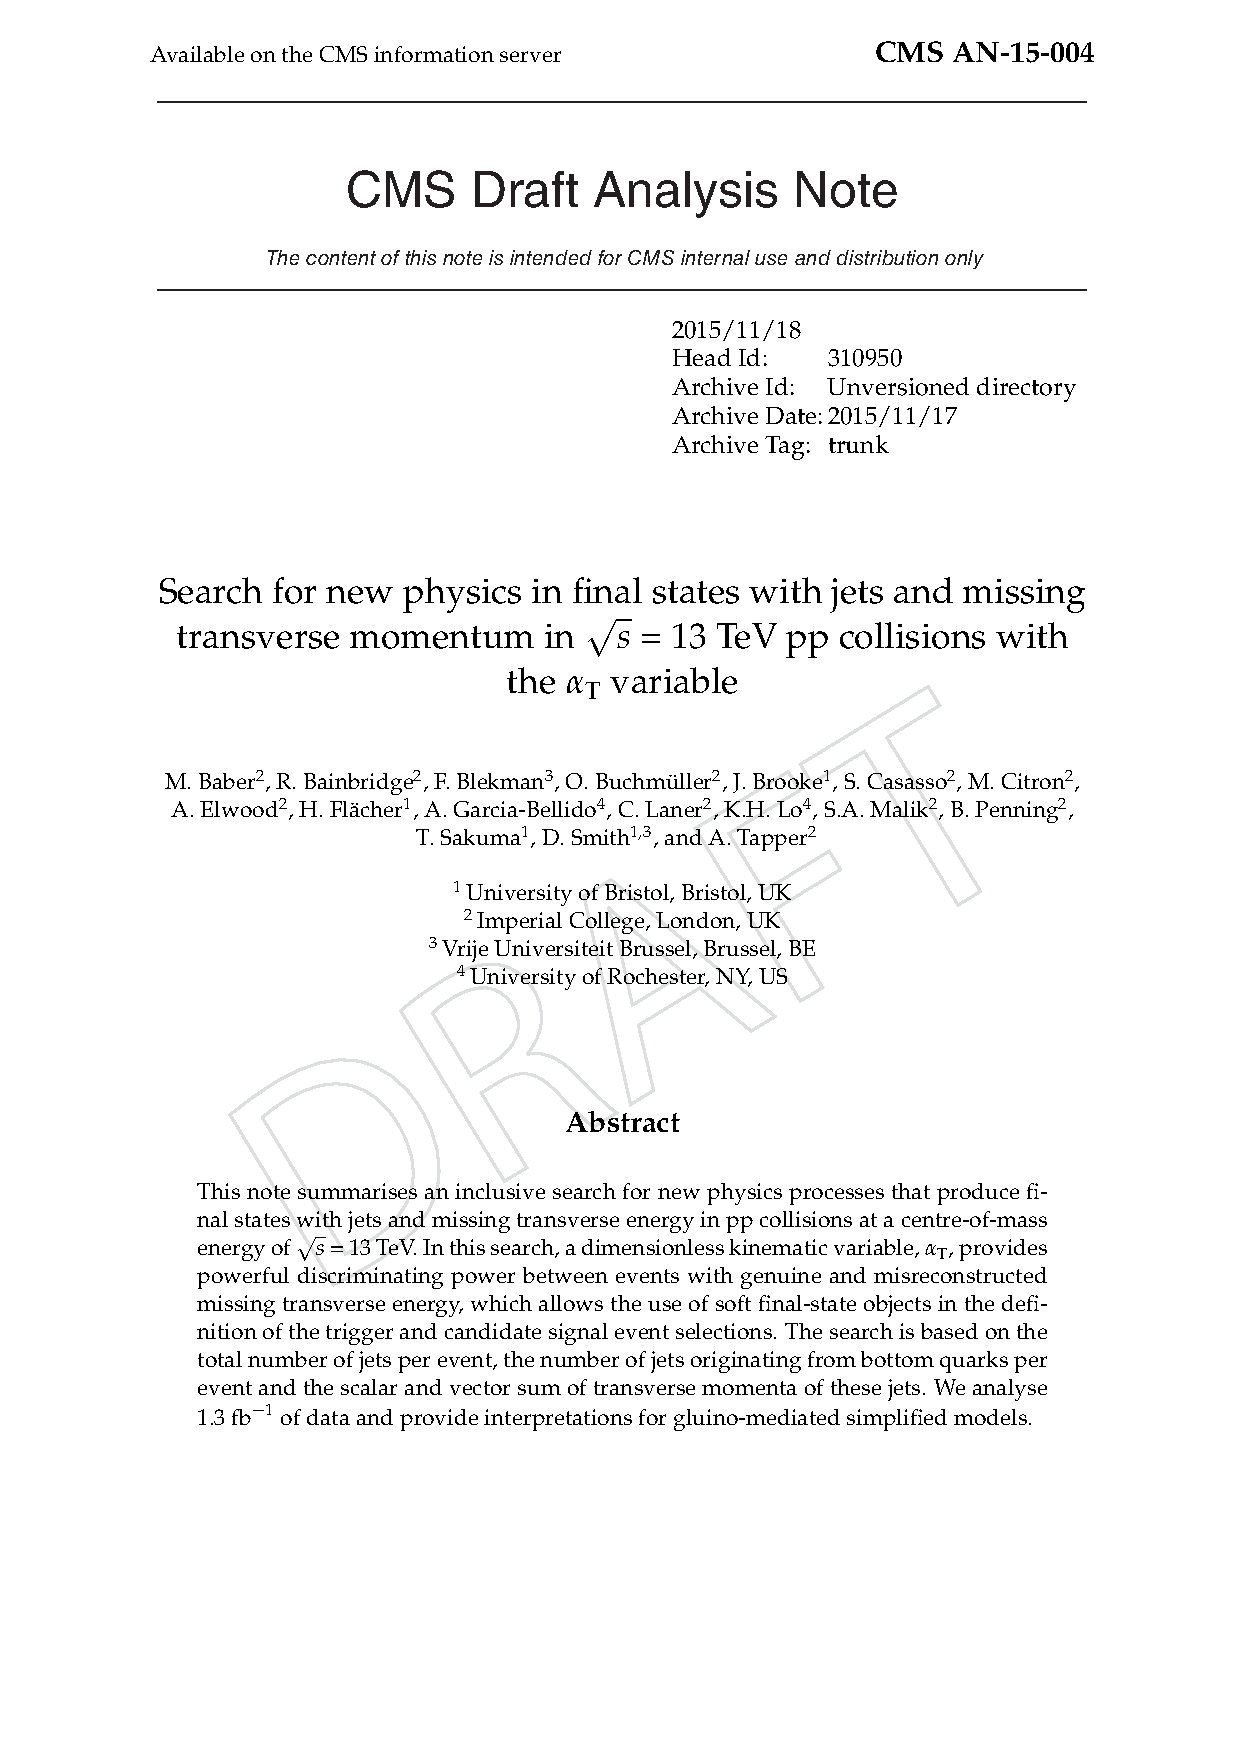
\includegraphics[width=0.5\textwidth]{figures/DMplots/bla.pdf}}
%\subfigure{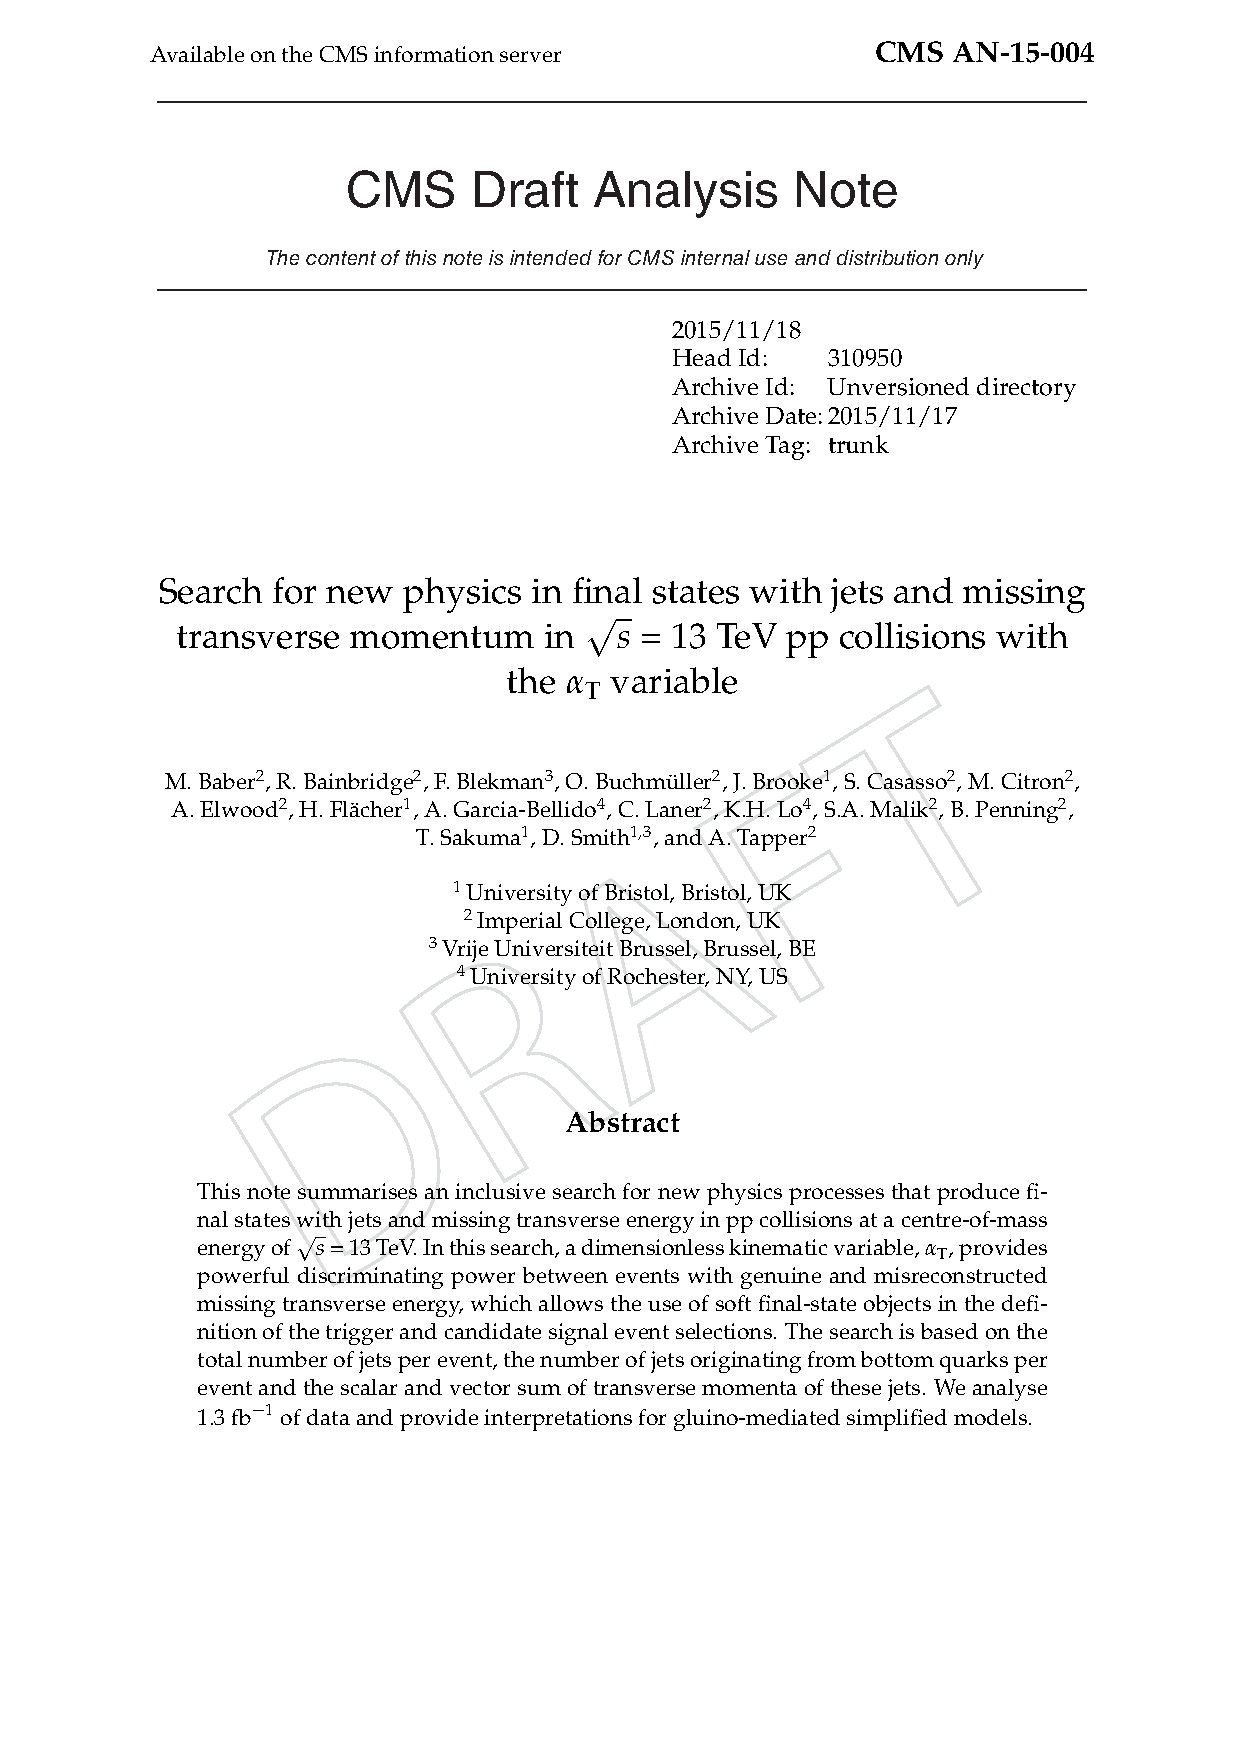
\includegraphics[width=0.5\textwidth]{figures/DMplots/bla.pdf}}
%\caption{\label{fig:limits_S} Expected exclusion contours at 95\% CL for
%3\fbinv and 10\fbinv using scalar couplings. } \end{figure}


\clearpage \subsection{Heavy flavour models} \label{sec:dm_heavyjet}

Owing to the principal of Minimal Flavor Violation (MFV), top and bottom quarks
can play important roles in the phenomenology of dark matter. Scalar and
pseudoscalar models predict not only the `monojet' processes described in
Sec.~\ref{sec:dm_lightjet} but also the production of dark matter in association
with top (or bottom) pairs. This results in signatures with relatively large jet
multiplicities, in particular for \DMtt production. The \alphat analysis is well 
suited to searching for such signatures. An example Feynman diagram for the pair
production of dark matter particles in association with pairs of heavy quarks is
shown in Fig.~\ref{fig:feynman_hf}.


\begin{figure}[h!] \centering
\subfigure{\includegraphics[width=0.35\textwidth]{figures/DMplots/feynman_hf.pdf}}
\caption{Feynman diagram of the pair production of Dark Matter particles in
association with $t\bar{t}$ or $b\bar{b}$. \cite{Abercrombie:2015wmb}}
\label{fig:feynman_hf} \end{figure}


The cross sections, signal yields and efficiencies for scalar and pseudoscalar
\DMtt models expected with 2~\ifb of data are shown in 
Tables~\ref{summaryTableAN_DMttP_xs10_2p1fb_exp}~and~\ref{summaryTableAN_DMttS_xs10_2p1fb_exp} for \DMtt. 

The selection efficiencies for these models are around $\sim 10$\%, and the improvement
provided by the new asymmetric and monojet categories is again evident.

\clearpage 
\input{tables/DM/summaryTableAN_DMttP_xs10_2p1fb_exp.tex}
\input{tables/DM/summaryTableAN_DMttS_xs10_2p1fb_exp.tex} 
\clearpage


The yields and efficiencies for \DMbb are shown in Tables~\ref{summaryTableAN_DMbbP_xs10_2p1fb_exp}~and~\ref{summaryTableAN_DMbbS_xs10_2p1fb_exp}, respectively. 
\begin{table}
\small
\centering
\begin{tabular}{lllllll}
\label{summaryTableAN_DMbbP_xs10_2p1fb_exp}
\hline
$m_\phi$ & $m_\chi$ & $\sigma$ [pb] & Yield (sym) & Yield (asy) & Yield (mon) & Efficiency [\%] \\ \hline
1000      &   1000      &   2.31e-09  &   0.00      &   0.00      &   0.00      &   12.97     \\ 
10        &   1000      &   1.52e-09  &   0.00      &   0.00      &   0.00      &   13.18     \\ 
100       &   10        &   5.36e-01  &   0.08      &   0.17      &   0.61      &   0.08      \\ 
10        &   10        &   9.36e-02  &   0.00      &   0.01      &   0.02      &   0.01      \\ 
15        &   10        &   1.30e-01  &   0.00      &   0.01      &   0.02      &   0.01      \\ 
50        &   10        &   1.94e+00  &   0.04      &   0.11      &   0.50      &   0.02      \\ 
200       &   150       &   1.52e-04  &   0.00      &   0.00      &   0.00      &   1.46      \\ 
295       &   150       &   1.67e-03  &   0.01      &   0.01      &   0.02      &   1.03      \\ 
500       &   150       &   1.26e-03  &   0.01      &   0.01      &   0.04      &   2.11      \\ 
1000      &   1         &   5.48e-05  &   0.00      &   0.00      &   0.00      &   4.22      \\ 
100       &   1         &   5.37e-01  &   0.04      &   0.21      &   0.79      &   0.09      \\ 
10        &   1         &   6.25e+00  &   0.02      &   0.01      &   0.22      &   0.00      \\ 
200       &   1         &   8.59e-02  &   0.10      &   0.15      &   0.40      &   0.36      \\ 
20        &   1         &   4.82e+00  &   0.00      &   0.00      &   0.27      &   0.00      \\ 
300       &   1         &   2.25e-02  &   0.04      &   0.08      &   0.27      &   0.82      \\ 
500       &   1         &   1.51e-03  &   0.01      &   0.01      &   0.04      &   1.89      \\ 
50        &   1         &   1.95e+00  &   0.07      &   0.17      &   0.31      &   0.01      \\ 
10        &   500       &   2.12e-07  &   0.00      &   0.00      &   0.00      &   7.26      \\ 
500       &   500       &   3.10e-07  &   0.00      &   0.00      &   0.00      &   7.30      \\ 
995       &   500       &   6.70e-06  &   0.00      &   0.00      &   0.00      &   6.17      \\ 
10        &   50        &   3.19e-03  &   0.00      &   0.00      &   0.01      &   0.20      \\ 
200       &   50        &   8.56e-02  &   0.09      &   0.14      &   0.39      &   0.34      \\ 
50        &   50        &   4.19e-03  &   0.00      &   0.00      &   0.01      &   0.21      \\ 
95        &   50        &   2.21e-02  &   0.01      &   0.02      &   0.03      &   0.12      \\ 
\hline
\end{tabular}
\caption{Cross section, yields at 2~\ifb (split according to symmetric, asymmetric, and monojet categories), and total selection efficiency for the pseudo-scalar \DMbb samples.}
\label{summaryTableAN_DMbbP_xs10_2p1fb_exp}
\end{table}

\begin{table}
\small
\label{summaryTableAN_DMbbS_xs10_2p1fb_exp}
\centering
\begin{tabular}{lllllll}
\hline
$m_\phi$ & $m_\chi$ & $\sigma$ [pb] & Yield (sym) & Yield (asy) & Yield (mon) & Efficiency [\%] \\ \hline
1000      &   1000      &   4.09e-10  &   0.00      &   0.00      &   0.00      &   13.48     \\ 
10        &   1000      &   2.88e-10  &   0.00      &   0.00      &   0.00      &   13.87     \\ 
100       &   10        &   1.24e+00  &   0.29      &   0.32      &   1.41      &   0.08      \\ 
10        &   10        &   2.68e-01  &   0.01      &   0.03      &   0.07      &   0.02      \\ 
15        &   10        &   3.52e-01  &   0.02      &   0.04      &   0.10      &   0.02      \\ 
50        &   10        &   7.66e+00  &   0.29      &   0.81      &   2.34      &   0.02      \\ 
200       &   150       &   5.91e-05  &   0.00      &   0.00      &   0.00      &   1.78      \\ 
295       &   150       &   2.58e-04  &   0.00      &   0.00      &   0.00      &   1.43      \\ 
500       &   150       &   1.50e-03  &   0.01      &   0.01      &   0.04      &   2.04      \\ 
1000      &   1         &   5.41e-05  &   0.00      &   0.00      &   0.00      &   4.44      \\ 
100       &   1         &   1.25e+00  &   0.37      &   0.49      &   1.75      &   0.10      \\ 
200       &   1         &   1.31e-01  &   0.08      &   0.23      &   0.63      &   0.34      \\ 
20        &   1         &   4.07e+01  &   0.00      &   1.41      &   0.56      &   0.00      \\ 
300       &   1         &   2.93e-02  &   0.06      &   0.11      &   0.32      &   0.79      \\ 
500       &   1         &   2.21e-03  &   0.01      &   0.02      &   0.06      &   2.00      \\ 
50        &   1         &   7.66e+00  &   0.87      &   0.44      &   1.10      &   0.02      \\ 
10        &   500       &   5.36e-08  &   0.00      &   0.00      &   0.00      &   8.61      \\ 
500       &   500       &   7.40e-08  &   0.00      &   0.00      &   0.00      &   8.27      \\ 
995       &   500       &   6.51e-07  &   0.00      &   0.00      &   0.00      &   6.72      \\ 
10        &   50        &   2.71e-03  &   0.00      &   0.00      &   0.01      &   0.32      \\ 
50        &   50        &   3.37e-03  &   0.00      &   0.01      &   0.01      &   0.29      \\ 
95        &   50        &   1.04e-02  &   0.01      &   0.01      &   0.03      &   0.19      \\ 
\hline
\end{tabular}
\caption{Cross section, yields at 2~\ifb (split according to symmetric, asymmetric, and monojet categories), and total selection efficiency for the pseudo-scalar \DMtt samples.}
\label{summaryTableAN_DMbbS_xs10_2p1fb_exp}
\end{table}
 
\clearpage


\subsubsection{Expected and observed sensitivities for DM+$t\bar{t}$}

The expected 95\% CL signal strength limits for simplified \DMtt models with scalar and
pseudo-scalar couplings are calculated for 2~\ifb. An uncertainty of 20\% is assumed for all 
heavy quark samples.


%These are shown in Tables~\ref{tab:dm_DMttS_2fb_limits}~and~\ref{tab:dm_DMttP_2fb_limits}. At this
%integrated luminosity, the sensitivity approaches scalar mediator masses of up 
%to 100~GeV and DM masses of about 10 GeV, whereas it is insufficient to
%significantly exclude the pseudoscalar model, which has generally smaller cross
%sections.

%Figure~\ref{fig:dm_DMttS_2fb_2dlimits} shows the interpolated scalar expected exclusion contour in the {\mphi-\mchi} mass plane.


\clearpage
Expected limits obtained for DM+$t\bar{t}$ are given in Tables~\ref{limits_DMttP_xs10_2p1fb_exp}-\ref{limits_DMttS_xs10_2p1fb_exp}, corresponding observed limits are shown in Tables~\ref{limits_DMttP_xs10_2p1fb_obs}-\ref{limits_DMttS_xs10_2p1fb_obs}.
\begin{table}
\begin{center}
\caption{DMttP 2.1\ifb exp 95\% CL upper limits}
\begin{tabular}{lcccccccc}
\label{limits_DMttP_xs10_2p1fb_exp}
\multirow{5}{*}{\rotatebox{90}{$m_{\rm{DM}}$ (GeV)}}
& \multicolumn{1}{c|}{500} &  &  &  &  &  &  & 2.83e+04\\ 
& \multicolumn{1}{c|}{150} &  &  &  &  & 509.12 &  & 37.06\\ 
& \multicolumn{1}{c|}{50} &  &  & 116.37 &  & 3.90 & 7.22 & \\ 
& \multicolumn{1}{c|}{10} & 42.02 &  & 2.27 & 2.80 &  &  & \\ 
& \multicolumn{1}{c|}{1} & 1.83 & 2.21 & 2.37 & 2.69 & 4.15 & 5.98 & 35.21\\ 
\cline{2-9}
& \multicolumn{1}{c|}{} & 10 & 20 & 50 & 100 & 200 & 300 & 500\\ 
& & \multicolumn{6}{c}{$M_{\rm{Med}}$ (GeV)}
\end{tabular}
\end{center}
\end{table}


\begin{table}
\begin{center}
\caption{DMttS xs10 2p1fb exp 95\% CL upper limits}
\begin{tabular}{lccccccccc}
\label{limits_DMttS_xs10_2p1fb_exp}
\multirow{5}{*}{\rotatebox{90}{$m_{\rm{DM}}$ (GeV)}}
& \multicolumn{1}{c|}{500} &  &  &  &  &  &  & 9.38e+04 & \\ 
& \multicolumn{1}{c|}{150} &  &  &  &  & 1.24e+03 &  & 42.92 & \\ 
& \multicolumn{1}{c|}{50} &  &  & 207.56 &  & 4.29 & 8.25 &  & \\ 
& \multicolumn{1}{c|}{10} & 24.40 &  & 0.89 & 1.97 &  &  &  & \\ 
& \multicolumn{1}{c|}{1} & 0.38 & 0.49 & 0.77 & 2.06 & 4.97 & 8.77 & 34.88 & 304.60\\ 
\cline{2-10}
& \multicolumn{1}{c|}{} & 10 & 20 & 50 & 100 & 200 & 300 & 500 & 1000\\ 
& & \multicolumn{7}{c}{$M_{\rm{Med}}$ (GeV)}
\end{tabular}
\end{center}
\end{table}


\begin{table}
\begin{center}
\caption{DMttP xs10 2p1fb obs 95\% CL upper limits}
\begin{tabular}{lcccccccc}
\label{limits_DMttP_xs10_2p1fb_obs}
\multirow{5}{*}{\rotatebox{90}{$m_{\rm{DM}}$ (GeV)}}
& \multicolumn{1}{c|}{500} &  &  &  &  &  &  & 4.79e+04\\ 
& \multicolumn{1}{c|}{150} &  &  &  &  & 710.48 &  & 78.72\\ 
& \multicolumn{1}{c|}{50} &  &  & 149.04 &  & 8.18 & 10.45 & \\ 
& \multicolumn{1}{c|}{10} & 67.24 &  & 3.15 & 5.38 &  &  & \\ 
& \multicolumn{1}{c|}{1} & 3.03 & 4.43 & 3.38 & 4.65 & 5.96 & 10.28 & 58.06\\ 
\cline{2-9}
& \multicolumn{1}{c|}{} & 10 & 20 & 50 & 100 & 200 & 300 & 500\\ 
& & \multicolumn{6}{c}{$M_{\rm{Med}}$ (GeV)}
\end{tabular}
\end{center}
\end{table}


\begin{table}
\begin{center}
\caption{DMttS xs10 2p1fb obs 95\% CL upper limits}
\begin{tabular}{lccccccccc}
\label{limits_DMttS_xs10_2p1fb_obs}
\multirow{5}{*}{\rotatebox{90}{$m_{\rm{DM}}$ (GeV)}}
& \multicolumn{1}{c|}{500} &  &  &  &  &  &  & 1.37e+05 & \\ 
& \multicolumn{1}{c|}{150} &  &  &  &  & 2.53e+03 &  & 75.92 & \\ 
& \multicolumn{1}{c|}{50} &  &  & 466.29 &  & 9.64 & 17.03 &  & \\ 
& \multicolumn{1}{c|}{10} & 40.07 &  & 1.33 & 4.20 &  &  &  & \\ 
& \multicolumn{1}{c|}{1} & 0.45 & 0.99 & 1.27 & 3.99 & 11.27 & 14.34 & 47.10 & 539.73\\ 
\cline{2-10}
& \multicolumn{1}{c|}{} & 10 & 20 & 50 & 100 & 200 & 300 & 500 & 1000\\ 
& & \multicolumn{7}{c}{$M_{\rm{Med}}$ (GeV)}
\end{tabular}
\end{center}
\end{table}




Appendix~\ref{sec:dm_checklist} contains additional validation of the \DMj DM samples like signal and background yields for the most sensitive bins and sensitivities.

\subsubsection{Expected and observed sensitivities for DM+$b(\bar{b})$}

The expected 95\% CL signal strength limits for simplified DM+$t(\bar{t})$ models with scalar and
pseudo-scalar couplings are calculated for 2~\ifb. An uncertainty of 20\% is assumed for all 
heavy quark samples.


Figure~\ref{fig:dm_DMttS_2fb_2dlimits} shows the interpolated scalar expected 
exclusion contour in the {\mphi-\mchi} mass plane.


\clearpage
Expected limits obtained for DM+$t\bar{t}$ are given in Tables~\ref{limits_DMbbP_xs10_2p1fb_exp}-\ref{limits_DMbbS_xs10_2p1fb_exp}, corresponding observed limits are shown in Tables~\ref{limits_DMbbP_xs10_2p1fb_obs}-\ref{limits_DMbbS_xs10_2p1fb_ob}.
\begin{table}
\begin{center}
\tiny
\caption{DMbbP 2.1\ifb exp 95\% CL upper limits}
\begin{tabular}{lccccccccccccc}
\label{limits_DMbbP_xs10_2p1fb_exp}
\multirow{6}{*}{\rotatebox{90}{$m_{\rm{DM}}$ (GeV)}}
& \multicolumn{1}{c|}{1000} & 2.03e+08 &  &  &  &  &  &  &  &  &  &  & 1.44e+08\\ 
& \multicolumn{1}{c|}{500} & 3.76e+06 &  &  &  &  &  &  &  &  & 2.79e+06 & 1.67e+05 & \\ 
& \multicolumn{1}{c|}{150} &  &  &  &  &  &  & 3.14e+04 & 5.07e+03 &  & 3.16e+03 &  & \\ 
& \multicolumn{1}{c|}{50} & 6.87e+03 &  &  & 5.53e+03 & 1.50e+03 &  & 162.84 &  &  &  &  & \\ 
& \multicolumn{1}{c|}{10} & 1.60e+03 & 827.41 &  & 156.65 &  & 105.24 &  &  &  &  &  & \\ 
& \multicolumn{1}{c|}{1} & 177.94 &  & 78.47 & 70.34 &  & 93.38 & 180.58 &  & 415.85 & 2.64e+03 &  & 3.36e+04\\ 
\cline{2-14}
& \multicolumn{1}{c|}{} & 10 & 15 & 20 & 50 & 95 & 100 & 200 & 295 & 300 & 500 & 995 & 1000\\ 
& & \multicolumn{11}{c}{$M_{\rm{Med}}$ (GeV)}
\end{tabular}
\end{center}
\end{table}

\begin{table}
\begin{center}
\tiny
\caption{DMbbS xs10 2p1fb exp 95\% CL upper limits}
\begin{tabular}{lccccccccccccc}
\label{limits_DMbbS_xs10_2p1fb_exp}
\multirow{6}{*}{\rotatebox{90}{$m_{\rm{DM}}$ (GeV)}}
& \multicolumn{1}{c|}{1000} & 1.03e+09 &  &  &  &  &  &  &  &  &  &  & 7.52e+08\\ 
& \multicolumn{1}{c|}{500} & 1.27e+07 &  &  &  &  &  &  &  &  & 1.08e+07 & 1.48e+06 & \\ 
& \multicolumn{1}{c|}{150} &  &  &  &  &  &  & 6.97e+04 & 2.12e+04 &  & 2.72e+03 &  & \\ 
& \multicolumn{1}{c|}{50} & 7.24e+03 &  &  & 5.96e+03 & 2.09e+03 &  &  &  &  &  &  & \\ 
& \multicolumn{1}{c|}{10} & 828.51 & 210.29 &  & 24.07 &  & 43.11 &  &  &  &  &  & \\ 
& \multicolumn{1}{c|}{1} & -1.00 &  & 21.19 & 11.30 &  & 38.25 & 161.04 &  & 290.34 & 1.85e+03 &  & 3.10e+04\\ 
\cline{2-14}
& \multicolumn{1}{c|}{} & 10 & 15 & 20 & 50 & 95 & 100 & 200 & 295 & 300 & 500 & 995 & 1000\\ 
& & \multicolumn{11}{c}{$M_{\rm{Med}}$ (GeV)}
\end{tabular}
\end{center}
\end{table}


\begin{table}
\tiny
\begin{center}
\caption{DMbbP xs10 2p1fb obs 95\% CL upper limits}
\begin{tabular}{lccccccccccccc}
\label{limits_DMbbP_xs10_2p1fb_obs}
\multirow{6}{*}{\rotatebox{90}{$m_{\rm{DM}}$ (GeV)}}
& \multicolumn{1}{c|}{1000} & 3.41e+08 &  &  &  &  &  &  &  &  &  &  & 2.04e+08\\ 
& \multicolumn{1}{c|}{500} & 4.68e+06 &  &  &  &  &  &  &  &  & 3.95e+06 & 2.12e+05 & \\ 
& \multicolumn{1}{c|}{150} &  &  &  &  &  &  & 6.05e+04 & 6.78e+03 &  & 5.75e+03 &  & \\ 
& \multicolumn{1}{c|}{50} & 6.69e+03 &  &  & 5.39e+03 & 1.29e+03 &  & 232.75 &  &  &  &  & \\ 
& \multicolumn{1}{c|}{10} & 1.93e+03 & 966.61 &  & 239.84 &  & 111.76 &  &  &  &  &  & \\ 
& \multicolumn{1}{c|}{1} & 381.09 &  & 55.43 & 79.27 &  & 142.25 & 213.16 &  & 430.82 & 3.23e+03 &  & 6.82e+04\\ 
\cline{2-14}
& \multicolumn{1}{c|}{} & 10 & 15 & 20 & 50 & 95 & 100 & 200 & 295 & 300 & 500 & 995 & 1000\\ 
& & \multicolumn{11}{c}{$M_{\rm{Med}}$ (GeV)}
\end{tabular}
\end{center}
\end{table}

\begin{table}
\tiny
\begin{center}
\caption{DMbbS xs10 2p1fb obs 95\% CL upper limits}
\begin{tabular}{lccccccccccccc}
\label{limits_DMbbS_xs10_2p1fb_obs}
\multirow{6}{*}{\rotatebox{90}{$m_{\rm{DM}}$ (GeV)}}
& \multicolumn{1}{c|}{1000} & 1.23e+09 &  &  &  &  &  &  &  &  &  &  & 7.67e+08\\ 
& \multicolumn{1}{c|}{500} & 1.91e+07 &  &  &  &  &  &  &  &  & 8.84e+06 & 2.35e+06 & \\ 
& \multicolumn{1}{c|}{150} &  &  &  &  &  &  & 8.37e+04 & 4.18e+04 &  & 5.64e+03 &  & \\ 
& \multicolumn{1}{c|}{50} & 2.52e+04 &  &  & 1.42e+04 & 6.06e+03 &  &  &  &  &  &  & \\ 
& \multicolumn{1}{c|}{10} & 7.29e+03 & 1.32e+03 &  & 60.69 &  & 74.92 &  &  &  &  &  & \\ 
& \multicolumn{1}{c|}{1} & 3.55e+03 &  & 248.93 & 83.95 &  & 175.05 & 584.16 &  & 528.83 & 4.19e+03 &  & 4.70e+04\\ 
\cline{2-14}
& \multicolumn{1}{c|}{} & 10 & 15 & 20 & 50 & 95 & 100 & 200 & 295 & 300 & 500 & 995 & 1000\\ 
& & \multicolumn{11}{c}{$M_{\rm{Med}}$ (GeV)}
\end{tabular}
\end{center}
\end{table}



Appendix~\ref{sec:dm_checklist} contains additional validation for the \DMtt and \DMtt DM samples like signal and background yields for the most sensitive bins and sensitivities.
\subsubsection{Most sensitive bins for DM+$b(\bar{b})$}

%\section{Summary}
\label{sec:summary}

We report on the prospects for a missing energy plus jet search that
is sensitive to a wide range of potential dark matter models.
The analysis follows an inclusive approach designed to capture a wide
scope of possible final states, use of robust methods to be
insensitive to multijet production, instrumental effects and MC
mis-modelling. Thus making it ideal for early data discoveries.
The original $\alpha_\textrm{T}$ analysis has been considerably extended  been improved in several areas, 
including an increase in the acceptance of the signal region and an optimisation of
the signal event categorisation. By relaxing the minimal jet multiplicity 
to as well include single jet events and adding an orthogonal jet selection with a lower 
\Pt requirement on the second leading jet. This leads to 
significantly improved acceptance to compressed SUSY and Dark Matter
models.

Candidate signal events are binned according to the number of
reconstructed jets, the number of jets identified to originate from
bottom quarks, and the scalar and vector sums of the transverse energy
of jets. The sum of standard model backgrounds per bin is estimated
from a simultaneous binned likelihood fit to event yields in the
signal region and \mj, \mmj, and \gj control samples. The
analysis relies heavily on methods and cross-checks derived from the
data control samples to demonstrate control of the SM background
predictions. 


Preliminary projections are presented for DM
simplified models using currently recorded $\sqrt{s} =$ 13~TeV data and $2.1$\ifb of data.

\appendix
%\section{Dark Matter models validations}
\label{sec:dm_checklist}

\subsection{\DMj models}

Tables~\ref{mostSensitiveBins_DMV_NNPDF30_Vector_Mphi-10_Mchi-1_gSM-1p0_gDM-1p0_25ns.tex}-\ref{mostSensitiveBins_DMS_NNPDF30_Scalar_Mphi-500_Mchi-150_gSM-1p0_gDM-1p0_25ns.tex} summarises the five most sensitive (\njet,\nb,\scalht,\mht) bins, background and signal yield and significance for selected \DMbb masses for two mass points each vor vector, axial-vector, pseudo-scalar and scalar samples

As expected, the sensitivity for these models mostly lies at low jet
multiplicities, low-medium \scalht, and at \mht values close to the upper bound
of the relevant \scalht bin Note that the \mht dimension is not utilised within 
the monojet category. Also note that, for convenience, all signal models have 
been normalised to a cross section of 10 pb in these tables.




\begin{tabular}{|l|l|l|l|l|}
\footnotesize
   \label{mostSensitiveBins_DMV_NNPDF30_Vector_Mphi-10_Mchi-1_gSM-1p0_gDM-1p0_25ns}
	\textbf{DMV NNPDF30 Vector Mphi-10 Mchi-1 gSM-1p0 gDM-1p0 25ns mht}	 & 	bgTtw	 & 	bgZinv	 & 	Signal &	 Significance \\ 
	\hline
	htBin 600-800 cat ge5j eq1b mht 350 & 	2.43	 & 	1.16	 & 	0.00 	&0.000000 \\ 
	htBin 800-Inf cat ge5j eq0b mht 575 & 	0.55	 & 	1.71	 & 	0.00 	&0.000000 \\ 
	htBin 600-Inf cat eq4a eq1b mht 575 & 	0.02	 & 	0.08	 & 	0.00 	&0.000000 \\ 
	htBin 350-400 cat eq4j eq1b mht 0 & 	5.05	 & 	0.75	 & 	0.00 	&0.000000 \\ 
	htBin 350-400 cat ge5j eq1b mht 0 & 	2.24	 & 	0.28	 & 	0.00 	&0.000000 \\ 
\end{tabular}
\\
 \begin{tabular}{|l|l|l|l|l|}
\small
   \label{mostSensitiveBins_DMV_NNPDF30_Vector_Mphi-500_Mchi-150_gSM-1p0_gDM-1p0_25ns}
	\textbf{DMV NNPDF30 Vector Mphi-500 Mchi-150 gSM-1p0 gDM-1p0}	 & 	bgTtw	 & 	bgZinv	 & 	Signal &	 Significance \\ 
	\hline
	htBin 600-800 cat eq3j eq1b mht 525 & 	0.35	 & 	1.08	 & 	0.60 	&0.376317 \\ 
	htBin 800-Inf cat eq3j eq0b mht 575 & 	0.99	 & 	2.64	 & 	0.52 	&0.166584 \\ 
	htBin 800-Inf cat eq3j eq0b mht 425 & 	1.40	 & 	4.20	 & 	0.57 	&0.137786 \\ 
	htBin 400-500 cat eq2j eq1b mht 375 & 	2.48	 & 	4.18	 & 	0.40 	&0.102571 \\ 
	htBin 500-600 cat eq2j eq1b mht 575 & 	0.33	 & 	0.56	 & 	0.38 	&0.084309 \\ 
\end{tabular}
\\

 \begin{tabular}{|l|l|l|l|l|}
\small
   \label{mostSensitiveBins_DMV_NNPDF30_Axial_Mphi-10_Mchi-1_gSM-1p0_gDM-1p0_25ns}
   \textbf{DMV NNPDF30 Axial Mphi-10 Mchi-1 gSM-1p0 gDM-1p0}	 a& 	bgTtw	 & 	bgZinv	 & 	Signal &	 Significance \\ 
	\hline
	htBin 200-250 cat eq3a ge3b mht 0 & 	0.50	 & 	0.08	 & 	0.00 	&0.000000 \\ 
	htBin 600-800 cat ge5j eq1b mht 350 & 	2.43	 & 	1.16	 & 	0.00 	&0.000000 \\ 
	htBin 800-Inf cat ge5j eq0b mht 575 & 	0.55	 & 	1.71	 & 	0.00 	&0.000000 \\ 
	htBin 600-Inf cat eq4a eq1b mht 575 & 	0.02	 & 	0.08	 & 	0.00 	&0.000000 \\ 
	htBin 350-400 cat eq4j eq1b mht 0 & 	5.05	 & 	0.75	 & 	0.00 	&0.000000 \\ 
\end{tabular}

\\
 \begin{tabular}{|l|l|l|l|l|}
  \small
\label{mostSensitiveBins_DMV_NNPDF30_Axial_Mphi-500_Mchi-150_gSM-1p0_gDM-1p0_25ns}
	\textbf{DMV NNPDF30 Axial Mphi-500 Mchi-150 gSM-1p0 gDM-1p0}	 & 	bgTtw	 & 	bgZinv	 & 	Signal &	 Significance \\ 
	\hline
	htBin 600-800 cat eq4j eq0b mht 550 & 	1.12	 & 	3.44	 & 	0.72 	&0.174754 \\ 
	htBin 400-500 cat eq2a eq0b mht 475 & 	4.52	 & 	9.61	 & 	1.61 	&0.150429 \\ 
	htBin 500-600 cat eq3a eq0b mht 525 & 	1.02	 & 	2.66	 & 	0.40 	&0.140377 \\ 
	htBin 800-Inf cat ge5j eq1b mht 475 & 	0.46	 & 	0.40	 & 	0.33 	&0.105422 \\ 
	htBin 500-600 cat eq2a eq0b mht 0 & 	4.09	 & 	9.48	 & 	0.73 	&0.077469 \\ 
\end{tabular}
\\

\begin{tabular}{|l|l|l|l|l|}
\footnotesize
  \label{mostSensitiveBins_DMS_NNPDF30_Pseudoscalar_Mphi-10_Mchi-1_gSM-1p0_gDM-1p0_25ns}
	\textbf{DMS NNPDF30 Pseudoscalar Mphi-10 Mchi-1 gSM-1p0 gDM-1p0}	 & 	bgTtw	 & 	bgZinv	 & 	Signal &	 Significance \\ 
	\hline
	htBin 250-300 cat eq2a eq0b mht 275 & 	127.65	 & 	198.28	 & 	0.09 	&0.000725 \\ 
	htBin 200-250 cat eq3a eq0b mht 175 & 	382.80	 & 	352.12	 & 	0.10 	&0.000369 \\ 
	htBin 250-300 cat eq1j eq0b mht 0 & 	1334.66	 & 	2272.06	 & 	0.84 	&0.000257 \\ 
	htBin 200-250 cat eq2a eq0b mht 175 & 	1587.13	 & 	1778.80	 & 	0.35 	&0.000070 \\ 
	htBin 250-300 cat eq2j eq0b mht 225 & 	211.65	 & 	271.34	 & 	0.32 	&0.000061 \\ 
\end{tabular}
\\
\begin{tabular}{|l|l|l|l|l|}
\footnotesize
  \label{mostSensitiveBins_DMS_NNPDF30_Pseudoscalar_Mphi-500_Mchi-150_gSM-1p0_gDM-1p0_25ns}
	\textbf{DMS NNPDF30 Pseudoscalar Mphi-500 Mchi-150 gSM-1p0 gDM-1p0}	 & 	bgTtw	 & 	bgZinv	 & 	Signal &	 Significance \\ 
	\hline
	htBin 250-300 cat eq2j eq1b mht 0 & 	1.04	 & 	0.60	 & 	0.37 	&0.217363 \\ 
	htBin 800-Inf cat ge5j eq1b mht 525 & 	0.36	 & 	0.35	 & 	0.35 	&0.216671 \\ 
	htBin 600-800 cat ge5j eq0b mht 475 & 	1.14	 & 	2.47	 & 	0.70 	&0.176768 \\ 
	htBin 500-600 cat eq3a eq0b mht 525 & 	1.02	 & 	2.66	 & 	0.36 	&0.140377 \\ 
	htBin 600-800 cat eq3j eq1b mht 475 & 	0.93	 & 	0.91	 & 	0.19 	&0.097086 \\ 
\end{tabular}
\\

 \begin{tabular}{|l|l|l|l|l|}
\small
   \label{mostSensitiveBins_DMS_NNPDF30_Scalar_Mphi-10_Mchi-1_gSM-1p0_gDM-1p0_25ns}
	\textbf{DMS NNPDF30 Scalar Mphi-10 Mchi-1 gSM-1p0 gDM-1p0}	 & 	bgTtw	 & 	bgZinv	 & 	Signal &	 Significance \\ 
	\hline
	htBin 400-500 cat eq1j eq1b mht 0 & 	5.46	 & 	11.40	 & 	0.18 	&0.020358 \\ 
	htBin 200-250 cat eq2a eq0b mht 175 & 	1587.13	 & 	1778.80	 & 	0.39 	&0.000070 \\ 
	htBin 250-300 cat eq2j eq0b mht 225 & 	211.65	 & 	271.34	 & 	0.05 	&0.000061 \\ 
	htBin 200-250 cat eq1j eq0b mht 0 & 	4336.68	 & 	6239.23	 & 	0.64 	&0.000028 \\ 
	htBin 200-250 cat eq3a ge3b mht 0 & 	0.50	 & 	0.08	 & 	0.00 	&0.000000 \\ 
\end{tabular}

\\
 \begin{tabular}{|l|l|l|l|l|}
\small
   \label{mostSensitiveBins_DMS_NNPDF30_Scalar_Mphi-500_Mchi-150_gSM-1p0_gDM-1p0_25ns}
	\textbf{DMS NNPDF30 Scalar Mphi-500 Mchi-150 gSM-1p0 gDM-1p0 25ns mht}	 & 	bgTtw	 & 	bgZinv	 & 	Signal &	 Significance \\ 
	\hline
	htBin 600-800 cat eq2j eq0b mht 725 & 	0.38	 & 	1.30	 & 	0.36 	&0.203516 \\ 
	htBin 600-800 cat eq4j eq0b mht 550 & 	1.12	 & 	3.44	 & 	0.64 	&0.174754 \\ 
	htBin 800-Inf cat eq4j eq0b mht 675 & 	0.52	 & 	1.24	 & 	0.28 	&0.152232 \\ 
	htBin 600-800 cat eq4j eq0b mht 650 & 	0.43	 & 	1.35	 & 	0.28 	&0.140296 \\ 
	htBin 350-400 cat eq2j eq1b mht 325 & 	3.81	 & 	4.75	 & 	0.46 	&0.109951 \\ 
\end{tabular}
\\



\clearpage
\subsection{\DMbb and \DMtt models}



Tables~\ref{mostSensitiveBins_BBbarDMJets_pseudoscalar_Mchi-1_Mphi-10_25ns}-\ref{mostSensitiveBins_BBbarDMJets_scalar_Mchi-150_Mphi-500_25ns}.
show the five most sensitive bins, background and signal yield and significance for selected \DMbb masses.

 \begin{tabular}{|l|l|l|l|l|}
\small
   \label{mostSensitiveBins_BBbarDMJets_pseudoscalar_Mchi-1_Mphi-10_25ns}
	\textbf{BBbarDMJets pseudoscalar Mchi-1 Mphi-10}	 & 	bgTtw	 & 	bgZinv	 & 	Signal &	 Significance \\ 
	\hline
	htBin 200-250 cat eq1j eq0b mht 0 & 	4336.68	 & 	6239.23	 & 	0.18 	&0.000028 \\ 
	htBin 200-250 cat eq3a ge3b mht 0 & 	0.50	 & 	0.08	 & 	0.00 	&0.000000 \\ 
	htBin 600-800 cat ge5j eq1b mht 350 & 	2.43	 & 	1.16	 & 	0.00 	&0.000000 \\ 
	htBin 800-Inf cat ge5j eq0b mht 575 & 	0.55	 & 	1.71	 & 	0.00 	&0.000000 \\ 
	htBin 600-Inf cat eq4a eq1b mht 575 & 	0.02	 & 	0.08	 & 	0.00 	&0.000000 \\ 
\end{tabular}

\\
 \begin{tabular}{|l|l|l|l|l|}
\small
   \label{mostSensitiveBins_BBbarDMJets_pseudoscalar_Mchi-150_Mphi-500_25ns}
	\textbf{BBbarDMJets pseudoscalar Mchi-150 Mphi-500}	 & 	bgTtw	 & 	bgZinv	 & 	Signal &	 Significance \\ 
	\hline
	htBin 350-400 cat eq4a eq1b mht 300 & 	2.34	 & 	1.27	 & 	1.50 	&0.603291 \\ 
	htBin 200-250 cat eq2a eq2b mht 175 & 	8.86	 & 	7.42	 & 	4.29 	&0.571712 \\ 
	htBin 400-500 cat ge5a eq2b mht 250 & 	1.91	 & 	0.13	 & 	1.20 	&0.568945 \\ 
	htBin 250-300 cat eq2a eq2b mht 0 & 	2.01	 & 	1.76	 & 	1.24 	&0.532145 \\ 
	htBin 350-400 cat eq3a eq1b mht 275 & 	3.33	 & 	3.01	 & 	1.66 	&0.513233 \\ 
\end{tabular}
\\
 \begin{tabular}{|l|l|l|l|l|}
\small
   \label{mostSensitiveBins_BBbarDMJets_scalar_Mchi-1_Mphi-10_25ns}
	\textbf{BBbarDMJets scalar Mchi-1 Mphi-10}	 & 	bgTtw	 & 	bgZinv	 & 	Signal &	 Significance \\ 
	\hline
	htBin 600-800 cat ge5j eq1b mht 350 & 	2.43	 & 	1.16	 & 	0.00 	&0.000000 \\ 
	htBin 800-Inf cat ge5j eq0b mht 575 & 	0.55	 & 	1.71	 & 	0.00 	&0.000000 \\ 
	htBin 600-Inf cat eq4a eq1b mht 575 & 	0.02	 & 	0.08	 & 	0.00 	&0.000000 \\ 
	htBin 350-400 cat eq4j eq1b mht 0 & 	5.05	 & 	0.75	 & 	0.00 	&0.000000 \\ 
	htBin 800-Inf cat eq3j eq1b mht 675 & 	0.04	 & 	0.21	 & 	0.00 	&0.000000 \\ 
\end{tabular}
\\
 \begin{tabular}{|l|l|l|l|l|}
\small
   \label{mostSensitiveBins_BBbarDMJets_scalar_Mchi-150_Mphi-500_25ns}
	\textbf{BBbarDMJets scalar Mchi-150 Mphi-500}	 & 	bgTtw	 & 	bgZinv	 & 	Signal &	 Significance \\ 
	\hline
	htBin 200-250 cat eq2j eq2b mht 0 & 	0.97	 & 	0.93	 & 	2.28 	&1.273182 \\ 
	htBin 250-300 cat eq3a eq2b mht 250 & 	1.45	 & 	0.92	 & 	1.72 	&0.897552 \\ 
	htBin 400-500 cat eq3j eq1b mht 425 & 	1.60	 & 	1.72	 & 	1.81 	&0.789506 \\ 
	htBin 400-500 cat eq3j eq1b mht 275 & 	7.15	 & 	6.38	 & 	3.67 	&0.619530 \\ 
	htBin 500-600 cat ge5j ge3b mht 0 & 	1.13	 & 	0.04	 & 	1.20 	&0.579402 \\ 
\end{tabular}
\\

Most sensitive bins are large ($b$)-jet multiplicities, medium to high \scalht and \mht values. Note that, for convenience, all signal models have been normalised to a cross section of 10 pb in these tables.

\clearpage

Background and signal yields for the most sensitive bins for \DMtt samples are given in Tables~\ref{mostSensitiveBins_TTbarDMJets_pseudoscalar_Mchi-1_Mphi-10_25ns}-\ref{mostSensitiveBins_TTbarDMJets_scalar_Mchi-150_Mphi-500_25ns}.

As expected, the sensitivity for these models mostly lies at large jet and $b$-jet multiplicities, high \scalht as well as large \mht values. Also these tablesa are all normalised to $\sigma=10$\ipb


\begin{tabular}{|l|l|l|l|l|}
  \small
   \label{mostSensitiveBins_TTbarDMJets_pseudoscalar_Mchi-1_Mphi-10_25ns}
	\textbf{TTbarDMJets pseudoscalar Mchi-1 Mphi-10}	 & 	bgTtw	 & 	bgZinv	 & 	Signal &	 Significance \\ 
	\hline
	htBin 400-500 cat ge5j eq1b mht 300 & 	2.30	 & 	0.59	 & 	8.27 	&4.084547 \\ 
	htBin 600-800 cat ge5j eq2b mht 425 & 	0.19	 & 	0.04	 & 	5.54 	&3.958966 \\ 
	htBin 600-800 cat ge5j eq1b mht 450 & 	0.59	 & 	0.40	 & 	5.24 	&3.556865 \\ 
	htBin 400-500 cat ge5j eq2b mht 325 & 	0.43	 & 	0.08	 & 	5.05 	&3.519975 \\ 
	htBin 350-400 cat ge5a eq1b mht 300 & 	0.29	 & 	0.23	 & 	4.50 	&3.476202 \\ 
\end{tabular}
\\
 \begin{tabular}{|l|l|l|l|l|}
\small
   \label{mostSensitiveBins_TTbarDMJets_pseudoscalar_Mchi-150_Mphi-500_25ns}
	\textbf{TTbarDMJets pseudoscalar Mchi-150 Mphi-500}	 & 	bgTtw	 & 	bgZinv	 & 	Signal &	 Significance \\ 
	\hline
	htBin 600-800 cat ge5j eq1b mht 450 & 	0.59	 & 	0.40	 & 	35.12 	&24.867541 \\ 
	htBin 800-Inf cat ge5j eq1b mht 775 & 	0.09	 & 	0.39	 & 	23.55 	&18.646455 \\ 
	htBin 600-800 cat ge5j eq2b mht 325 & 	0.60	 & 	0.12	 & 	24.68 	&18.190695 \\ 
	htBin 600-800 cat ge5j eq1b mht 500 & 	0.27	 & 	0.34	 & 	23.81 	&18.032253 \\ 
	htBin 600-800 cat ge5j eq1b mht 400 & 	1.67	 & 	0.69	 & 	30.89 	&17.157983 \\ 
\end{tabular}
\\
\begin{tabular}{|l|l|l|l|l|}
\small
   \label{mostSensitiveBins_TTbarDMJets_scalar_Mchi-1_Mphi-10_25ns}
	\textbf{TTbarDMJets scalar Mchi-1 Mphi-10}	 & 	bgTtw	 & 	bgZinv	 & 	Signal &	 Significance \\ 
	\hline
	htBin 600-800 cat ge5j eq2b mht 275 & 	1.49	 & 	0.25	 & 	1.34 	&0.789106 \\ 
	htBin 350-400 cat eq3j eq2b mht 300 & 	0.85	 & 	0.13	 & 	1.33 	&0.717537 \\ 
	htBin 800-Inf cat ge5j eq1b mht 425 & 	0.63	 & 	0.41	 & 	1.32 	&0.676182 \\ 
	htBin 400-500 cat ge5a eq2b mht 200 & 	5.24	 & 	0.20	 & 	2.12 	&0.543026 \\ 
	htBin 400-500 cat eq4j eq1b mht 300 & 	7.80	 & 	2.75	 & 	2.54 	&0.532218 \\ 
\end{tabular}
\\
 \begin{tabular}{|l|l|l|l|l|}
\small
\label{mostSensitiveBins_TTbarDMJets_scalar_Mchi-150_Mphi-500_25ns}
	\textbf{TTbarDMJets scalar Mchi-150 Mphi-500}	 & 	bgTtw	 & 	bgZinv	 & 	Signal &	 Significance \\ 
	\hline
	htBin 800-Inf cat ge5j eq2b mht 725 & 	0.23	 & 	0.08	 & 	25.79 	&20.939012 \\ 
	htBin 600-800 cat ge5j eq2b mht 375 & 	0.47	 & 	0.13	 & 	26.05 	&19.598534 \\ 
	htBin 800-Inf cat ge5j eq1b mht 775 & 	0.09	 & 	0.39	 & 	24.14 	&18.646455 \\ 
	htBin 600-800 cat ge5j eq2b mht 525 & 	0.49	 & 	0.09	 & 	23.75 	&17.972944 \\ 
	htBin 600-800 cat ge5j eq2b mht 325 & 	0.60	 & 	0.12	 & 	20.36 	&15.194035 \\ 
\end{tabular}
\\


%%____________________________________________________________________________||
\bibliography{auto_generated}

%%____________________________________________________________________________||
%\appendix
%%%____________________________________________________________________________||
\section{Kinematic distributions for the signal region}
\label{sec:kisigplot}

This appendix shows distributions of events in the signal region in
each \scalht bin in each symmetric and asymmetric \njet bin for each
process as functions of 7 different variables, \ie, \alphat, \mht,
\bdphi, \met, the lead jet $\PT$, the second hardest jet $\PT$, and
\nb.

These distributions are show in 14 figures from Figure
\ref{c150107_s150318_f015_alphaT_100} to Figure
\ref{c150107_s150318_f015_nbjets_40}. The distributions of each
variable are shown in two figures: one for symmetric \njet bins and
the other for asymmetric \njet bins. Each figure contains 18 panels,
each shows the distribution in the specific \scalht bin and \njet bin
for all processes. These panels are arranged in 4 columns, for 4
different \njet bins, and 7 rows, for 7 different \scalht bins, and
share the axes.
\footnote{This type of data visualisation is called \textit{Trellis
    Graphics}
  (\url{http://ect.bell-labs.com/sl/project/trellis/wwww.html}), which
  was originally developed at the Bell Labs in 1990s. Trellis Graphics
  is particularly useful for examining multivariate categorical data
  \eg to find patters or correlations.}


In these figures, the event selection for the signal region described
in Section \ref{sec:selection} and summarised in tables
\ref{tab:pre-selections}, \ref{tab:alphat-thresholds}, and
\ref{tab:sr-selections} are applied. As described in Section
\ref{sec:preSelection}, the events in the symmetric \njet bins have
the second hardest jet with $\PT$ greater than 100\gev. The events in
the asymmetric \njet bins have the second hardest jet with $\PT$
between 40 and 100\gev.

From these figures, \eg the \nb distributions in Figures
\ref{c150107_s150318_f015_nbjets_100} and
\ref{c150107_s150318_f015_nbjets_40}, it can be seen that many \scalht
and \njet bins do not contain a multijet event. However, some bins do
contain many multijet events. For example, in Figure
\ref{c150107_s150318_f015_nbjets_40}, the bin for $350 < \scalht <
400\gev$ and $\njet = 3$ (the panel in the 4th row from the top and
the 2nd column from the left) has many multijet events at $\nb = 0$.
The origin of these multijet events will be clearer in distributions
shown in very fine bins of a histogram. For example, the panel in the
same position in Figure \ref{c150107_s150318_f015_biasedDPhi_40} shows
the distribution of the same set of events in very fine bins of
\bdphi. There, all multijet events are in a single bin of \bdphi.
These multijet events correspond to one MC event, weighed by a large
cross section of QCD. In Figures
\ref{c150107_s150318_f015_biasedDPhi_100} and
\ref{c150107_s150318_f015_biasedDPhi_40}, nearly all entries from
multijet events are very tall and contained in isolated bins \bdphi,
which indicates that these multijet events correspond a small number
of MC events.

Event filters and calibrations in the event reconstruction were still
actively developed when MC samples used in this note were generated.
We expect that many of these multijet events still we find in the
signal region will be removed when these filters or calibrations are
well tuned for Run~2 data.

On the other hand, as can be seen in Figure
\ref{c150107_s150318_f015_biasedDPhi_100}, many multijet events reside
in slightly above the cut applied on \bdphi in the highest \scalht and
high \njet bins. If these multijet events persist after the filters
and calibrations are tuned, they can be remove by raising the value of
\bdphi cut.





\begin{figure}[!h]
\centering
\includegraphics[scale=0.95]{figures/kiplots/c150107_s150318_f015_alphaT_100}
\caption{\textbf{\boldmath The \alphat distributions, symmetric \njet
bins:} The \alphat distributions of the events in the signal region in
each \scalht bin in each symmetric \njet bin for each process. Panels in
different rows show events in different \scalht bins. Panels in
different columns show events in different symmetric \njet bins.
Different processes are shown in different colors (or gray scales).}
\label{c150107_s150318_f015_alphaT_100}
\end{figure}

\begin{figure}[!h]
\centering
\includegraphics[scale=0.95]{figures/kiplots/c150107_s150318_f015_alphaT_40}
\caption{\textbf{\boldmath The \alphat distributions, asymmetric \njet
bins:} The \alphat distributions of the events in the signal region in
each \scalht bin in each asymmetric \njet bin for each process. Panels
in different rows show events in different \scalht bins. Panels in
different columns show events in different asymmetric \njet bins.
Different processes are shown in different colors (or gray scales).}
\label{c150107_s150318_f015_alphaT_40}
\end{figure}

\begin{figure}[!h]
\centering
\includegraphics[scale=0.95]{figures/kiplots/c150107_s150318_f015_MHT_100}
\caption{\textbf{\boldmath The \mht distributions, symmetric \njet
bins:} The \mht distributions of the events in the signal region in each
\scalht bin in each symmetric \njet bin for each process. Panels in
different rows show events in different \scalht bins. Panels in
different columns show events in different symmetric \njet bins.
Different processes are shown in different colors (or gray scales).}
\label{c150107_s150318_f015_MHT_100}
\end{figure}

\begin{figure}[!h]
\centering
\includegraphics[scale=0.95]{figures/kiplots/c150107_s150318_f015_MHT_40}
\caption{\textbf{\boldmath The \mht distributions, asymmetric \njet
bins:} The \mht distributions of the events in the signal region in each
\scalht bin in each asymmetric \njet bin for each process. Panels in
different rows show events in different \scalht bins. Panels in
different columns show events in different asymmetric \njet bins.
Different processes are shown in different colors (or gray scales).}
\label{c150107_s150318_f015_MHT_40}
\end{figure}

\begin{figure}[!h]
\centering
\includegraphics[scale=0.95]{figures/kiplots/c150107_s150318_f015_biasedDPhi_100}
\caption{\textbf{\boldmath The \bdphi distributions, symmetric \njet
bins:} The \bdphi distributions of the events in the signal region in
each \scalht bin in each symmetric \njet bin for each process. Panels in
different rows show events in different \scalht bins. Panels in
different columns show events in different symmetric \njet bins.
Different processes are shown in different colors (or gray scales).}
\label{c150107_s150318_f015_biasedDPhi_100}
\end{figure}

\begin{figure}[!h]
\centering
\includegraphics[scale=0.95]{figures/kiplots/c150107_s150318_f015_biasedDPhi_40}
\caption{\textbf{\boldmath The \bdphi distributions, asymmetric \njet
bins:} The \bdphi distributions of the events in the signal region in
each \scalht bin in each asymmetric \njet bin for each process. Panels
in different rows show events in different \scalht bins. Panels in
different columns show events in different asymmetric \njet bins.
Different processes are shown in different colors (or gray scales).}
\label{c150107_s150318_f015_biasedDPhi_40}
\end{figure}

\begin{figure}[!h]
\centering
\includegraphics[scale=0.95]{figures/kiplots/c150107_s150318_f015_MET_100}
\caption{\textbf{\boldmath The \met distributions, symmetric \njet
bins:} The \met distributions of the events in the signal region in each
\scalht bin in each symmetric \njet bin for each process. Panels in
different rows show events in different \scalht bins. Panels in
different columns show events in different symmetric \njet bins.
Different processes are shown in different colors (or gray scales).}
\label{c150107_s150318_f015_MET_100}
\end{figure}

\begin{figure}[!h]
\centering
\includegraphics[scale=0.95]{figures/kiplots/c150107_s150318_f015_MET_40}
\caption{\textbf{\boldmath The \met distributions, asymmetric \njet
bins:} The \met distributions of the events in the signal region in each
\scalht bin in each asymmetric \njet bin for each process. Panels in
different rows show events in different \scalht bins. Panels in
different columns show events in different asymmetric \njet bins.
Different processes are shown in different colors (or gray scales).}
\label{c150107_s150318_f015_MET_40}
\end{figure}

\begin{figure}[!h]
\centering
\includegraphics[scale=0.95]{figures/kiplots/c150107_s150318_f015_jet_pt_0_100}
\caption{\textbf{\boldmath The lead jet $\PT$ distributions, symmetric
\njet bins:} The lead jet $\PT$ distributions of the events in the
signal region in each \scalht bin in each symmetric \njet bin for each
process. Panels in different rows show events in different \scalht bins.
Panels in different columns show events in different symmetric \njet
bins. Different processes are shown in different colors (or gray
scales).} \label{c150107_s150318_f015_jet_pt_0_100}
\end{figure}

\begin{figure}[!h]
\centering
\includegraphics[scale=0.95]{figures/kiplots/c150107_s150318_f015_jet_pt_0_40}
\caption{\textbf{\boldmath The lead jet $\PT$ distributions, symmetric
\njet bins:} The lead jet $\PT$ distributions of the events in the
signal region in each \scalht bin in each asymmetric \njet bin for each
process. Panels in different rows show events in different \scalht bins.
Panels in different columns show events in different asymmetric \njet
bins. Different processes are shown in different colors (or gray
scales).} \label{c150107_s150318_f015_jet_pt_0_40}
\end{figure}

\begin{figure}[!h]
\centering
\includegraphics[scale=0.95]{figures/kiplots/c150107_s150318_f015_jet_pt_1_100}
\caption{\textbf{\boldmath The second hardest jet $\PT$ distributions,
symmetric \njet bins:} The second hardest jet $\PT$ distributions of the
events in the signal region in each \scalht bin in each symmetric \njet
bin for each process. Panels in different rows show events in different
\scalht bins. Panels in different columns show events in different
symmetric \njet bins. Different processes are shown in different colors
(or gray scales).} \label{c150107_s150318_f015_jet_pt_1_100}
\end{figure}

\begin{figure}[!h]
\centering
\includegraphics[scale=0.95]{figures/kiplots/c150107_s150318_f015_jet_pt_1_40}
\caption{\textbf{\boldmath The second hardest jet $\PT$ distributions,
asymmetric \njet bins:} The second hardest jet $\PT$ distributions of
the events in the signal region in each \scalht bin in each asymmetric
\njet bin for each process. Panels in different rows show events in
different \scalht bins. Panels in different columns show events in
different asymmetric \njet bins. Different processes are shown in
different colors (or gray scales).}
\label{c150107_s150318_f015_jet_pt_1_40}
\end{figure}

\begin{figure}[!h]
\centering
\includegraphics[scale=0.95]{figures/kiplots/c150107_s150318_f015_nbjets_100}
\caption{\textbf{\boldmath The \nb distributions, symmetric \njet bins:}
The $\nb$ distributions of the events in the signal region in each
\scalht bin in each symmetric \njet bin for each process. Panels in
different rows show events in different \scalht bins. Panels in
different columns show events in different symmetric \njet bins.
Different processes are shown in different colors (or gray scales).}
\label{c150107_s150318_f015_nbjets_100}
\end{figure}

\begin{figure}[!h]
\centering
\includegraphics[scale=0.95]{figures/kiplots/c150107_s150318_f015_nbjets_40}
\caption{\textbf{\boldmath The \nb distributions, asymmetric \njet bins:}
The $\nb$ distributions of the events in the signal region in each
\scalht bin in each asymmetric \njet bin for each process. Panels in
different rows show events in different \scalht bins. Panels in
different columns show events in different asymmetric \njet bins.
Different processes are shown in different colors (or gray scales).}
\label{c150107_s150318_f015_nbjets_40}
\end{figure}

%%____________________________________________________________________________||




